\documentclass{cheatsheet}
\usepackage{blindtext}
\usepackage{mdframed}
\usepackage{amsmath, amssymb, mathtools, empheq, physics}
\usepackage{ragged2e}

\newcommand{\dxt}{%
    \dot{x}
}

\newcommand{\ddxt}{%
    \ddot{x}
}

\newcommand{\dyt}{%
    \dot{y}
}

\newcommand{\ddyt}{%
    \ddot{y}
}
\newcommand{\ef}{%E-Feld
    \vec{E}
}

\newcommand{\bfe}{%B-Feld
    \vec{B}
}

\newcommand{\hf}{%H-Feld
    \vec{H}
}

\newcommand{\beispiel}[2]{
    \begin{tcolorbox}[
    title = \textbf{Beispiel: #1},
    colback = orange!10,
    colframe = orange!80
    ]
        #2
    \end{tcolorbox}
}

\newcommand{\formel}[2]{
    \begin{tcolorbox}[
    title = \textbf{Formel: #1},
    colback = PineGreen!10,
    colframe = PineGreen!70
    ]
        #2
    \end{tcolorbox}
}

\newcommand{\umbruch}{\vfill \null \columnbreak}


\newcommand{\WhiteSpace}[0]{
\begin{tcolorbox}[
		arc=0mm,
		colback=white,
		colframe=white,
		bottomrule = 0 mm,
		toprule = 0 mm,
		leftrule = 0 mm,
		rightrule = 0 mm,
		valign=center,
		left=0.5mm,
		top= -0.2 mm,
		bottom= -0.2 mm,
		fontupper=\color{white},
		before skip = 0mm,
		leftright skip = -0.5mm,
		after skip = 0 mm]
	
\end{tcolorbox}
}

\doctitle{Chemistry D-MAVT}
\geometry{a4paper,landscape,left=0.2cm,right=0.2cm, top=0.5cm, bottom=1.5cm}
\begin{document}

\section{Basics}
    \subsection{Conversions, Relations and Units}
\begin{minipage}[t]{0.23 \columnwidth}
\begin{itemize}[leftmargin=0.20cm, itemsep=0.05pt]
    \item mass: $[m] = kg$
    \item volume: $[V] = m^3$ 
    \item density: $\rho = \frac{m}{V}$\\
    $[\rho] = \frac{kg}{m^3}$
    \item ppm: $10^{-6}$
    \item ppb $10^{-9}$
    \item \# particles: $[n] = mol$
    \item molar mass: $[M] = \frac{kg}{mol}$
    \item molar volume (ideal gas):\\
    $V_mol = 22.41l$
\end{itemize}
\end{minipage}
\begin{minipage}[t]{0.23 \columnwidth}
\begin{itemize}[leftmargin=0.20cm, itemsep=0.05pt]
    \item mass \%: $\frac{m_i}{m_{tot}}$ 
    \item Avogardo's constant: \\
    $N_A = 6.022 \cdot 10^{23} \frac{1}{mol}$
    \item mol fraction: $[\chi] = \frac{mol}{mol}$
    \item molality: $[M_m] = \frac{mol}{kg}$
    \item molarity: $[M_v] = \frac{mol}{l}$
    \item length:\\
    $1$ \AA $= 10^{-10}m$
    \item amount of substance:\\
    $1 mol = 6.022 \cdot 10^{23}$
\end{itemize}
\end{minipage}
\begin{minipage}[t]{0.23 \columnwidth}
\begin{itemize}[leftmargin=0.20cm, itemsep=0.05pt]
    \item kinetic energy: \\
    $E_k = \frac{1}{2} m v^2$
    \item potential energy: \\
    $E_p = m g \Delta h$
    \item electrostatic pot. energy:\\
    $E_el = \frac{1}{4\pi \varepsilon_0} \frac{Q_1 Q_2}{d}$
    \item spec. heat capacity:\\
    $c_s = \frac{q}{m \Delta T}$
    \item energy of photon:\\
    $E = h \cdot \nu = \frac{h\cdot c}{\lambda}$
    \item Planck's constant:\\
    $6.626 \cdot 10^{-34} J \cdot s$
\end{itemize}
\end{minipage}
\begin{minipage}[t]{0.24 \columnwidth}
\begin{itemize}[leftmargin=0.20cm, itemsep=0.05pt]
    \item electron wavelength:\\
    $\lambda = \frac{h}{m_e \cdot v}$
    \item energy:\\
    $1 eV = 1.602 10^{-19} J$\\
    $1 cal = 4.18J$
    \item pressure:\\
    $1 Pa = 9.87 \cdot 10^{-6} atm$ \\
    $=1.0 \cdot 10^{-5} bar$\\
    $= 7.5 \cdot 10^{-3} torr$
    \item STP Ideal Gas Law:\\
    $0 ^\circ C = 273.15 K, 1 bar, 1 mol$
    \item STP Thermodynamics:\\
    $25^\circ C =298.15 K,1 bar,1 mol$
\end{itemize}
\end{minipage}
    \subsection{Common Ions}
\begin{minipage}{0.49 \columnwidth}
    \begin{center}
    \textbf{Common Anions}
        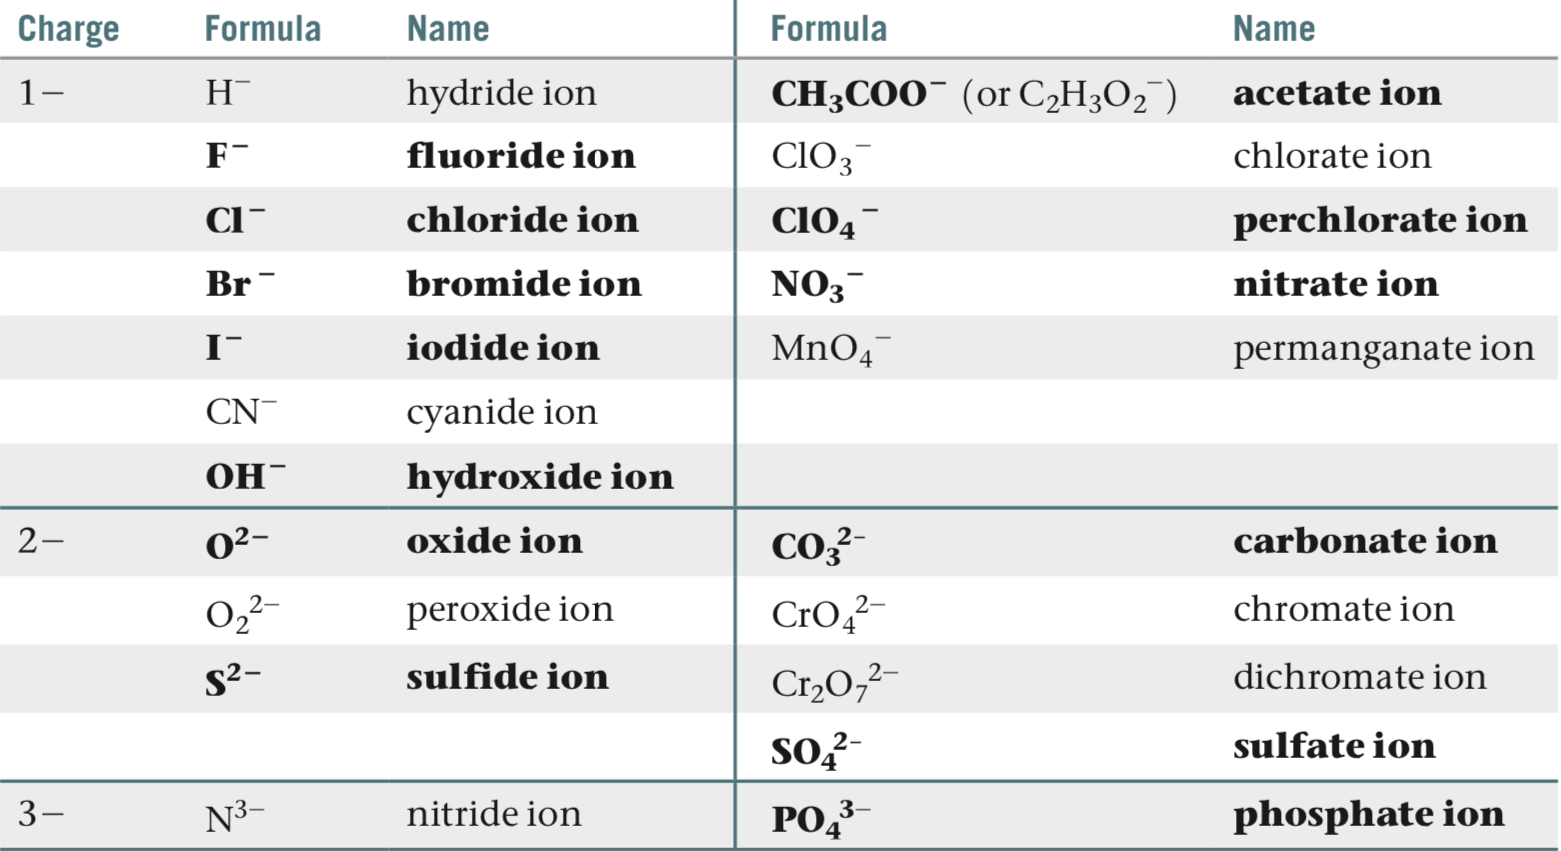
\includegraphics[width = \linewidth]{images/common_anions.jpeg}
    \end{center}
\end{minipage}
\begin{minipage}{0.49 \columnwidth}
    \begin{center}
    \textbf{Common Cations}
        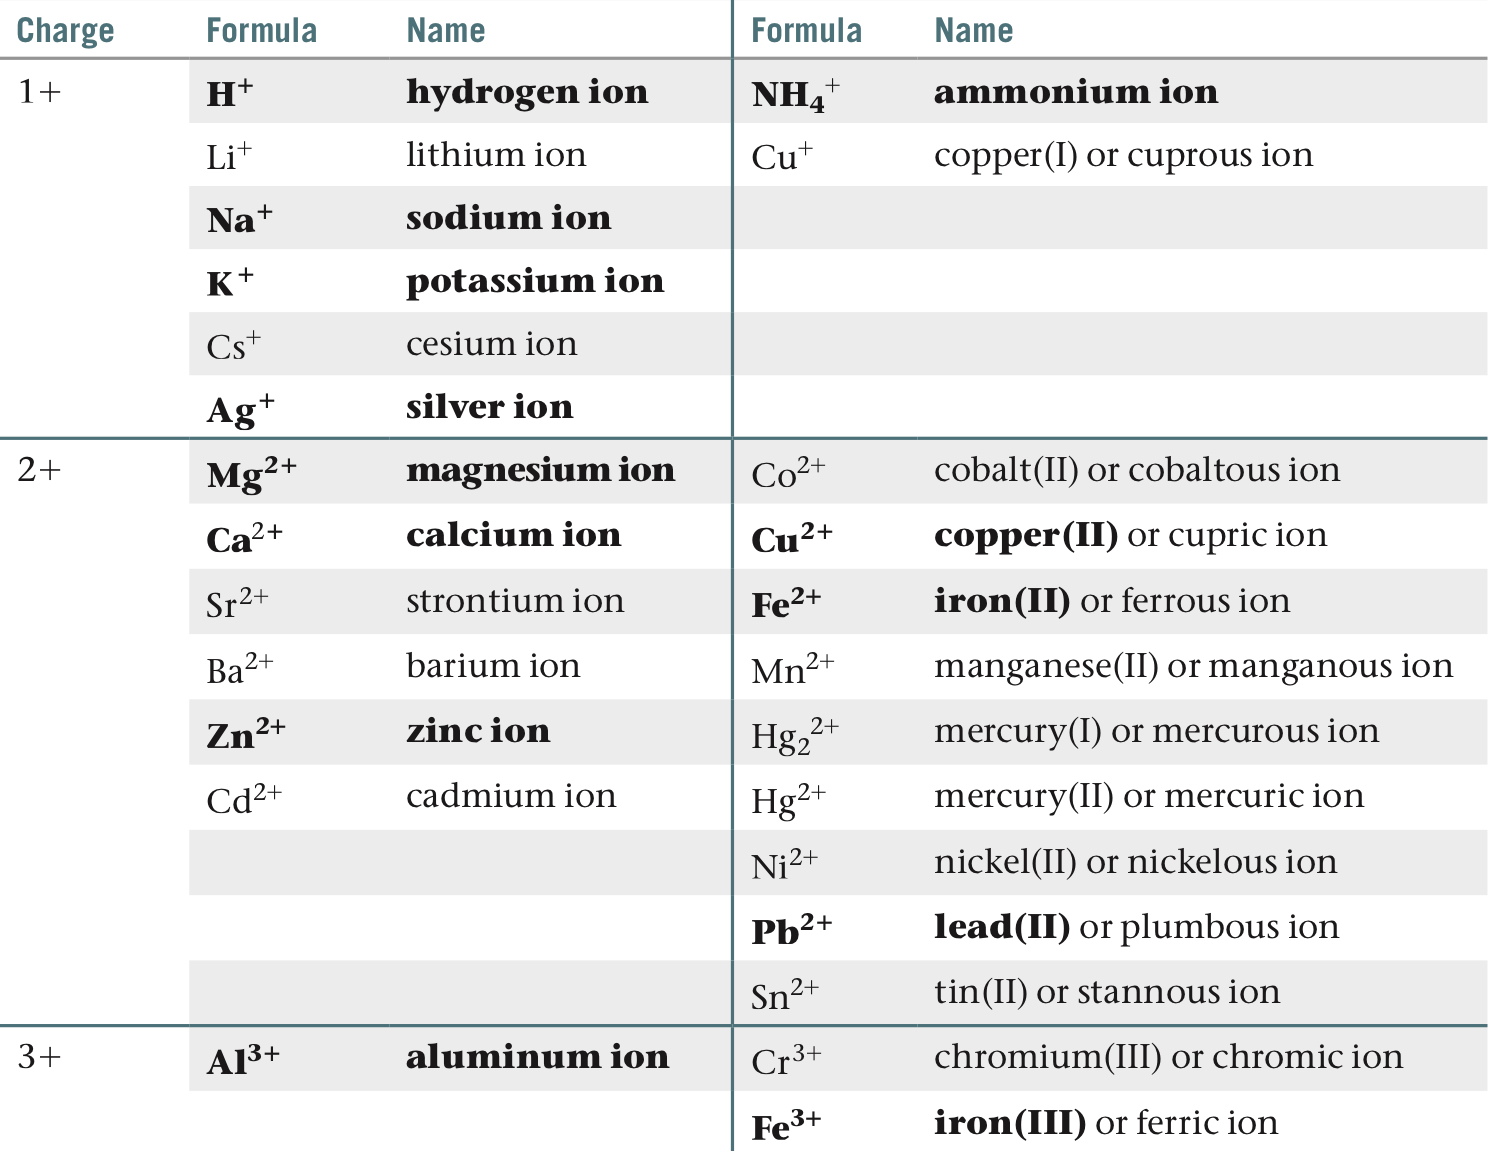
\includegraphics[width = \linewidth]{images/common _cations.jpeg}
    \end{center}
\end{minipage}
    \subsection{Trends in Periodic Table of Elements}{
\begin{minipage}{0.54\columnwidth}
    \begin{itemize}[leftmargin=0.20cm, itemsep=0.05pt]
        \item Due to "screening", valence electrons only feel effective charge $Z_{eff}$
        \item $Z_{eff}$ increases across a row
        \item Atomic size increases down a column (group) and decreases across row (period)
        \item Ionic radii: Ions are bigger down column
        \item Cations are smaller than neutral atom
        \item Anions are larger than neutral atom
        \item Ionization energy: Increases across period, decreases down group
    \end{itemize}
\end{minipage}
\begin{minipage}{0.45 \columnwidth}
    \begin{center}
        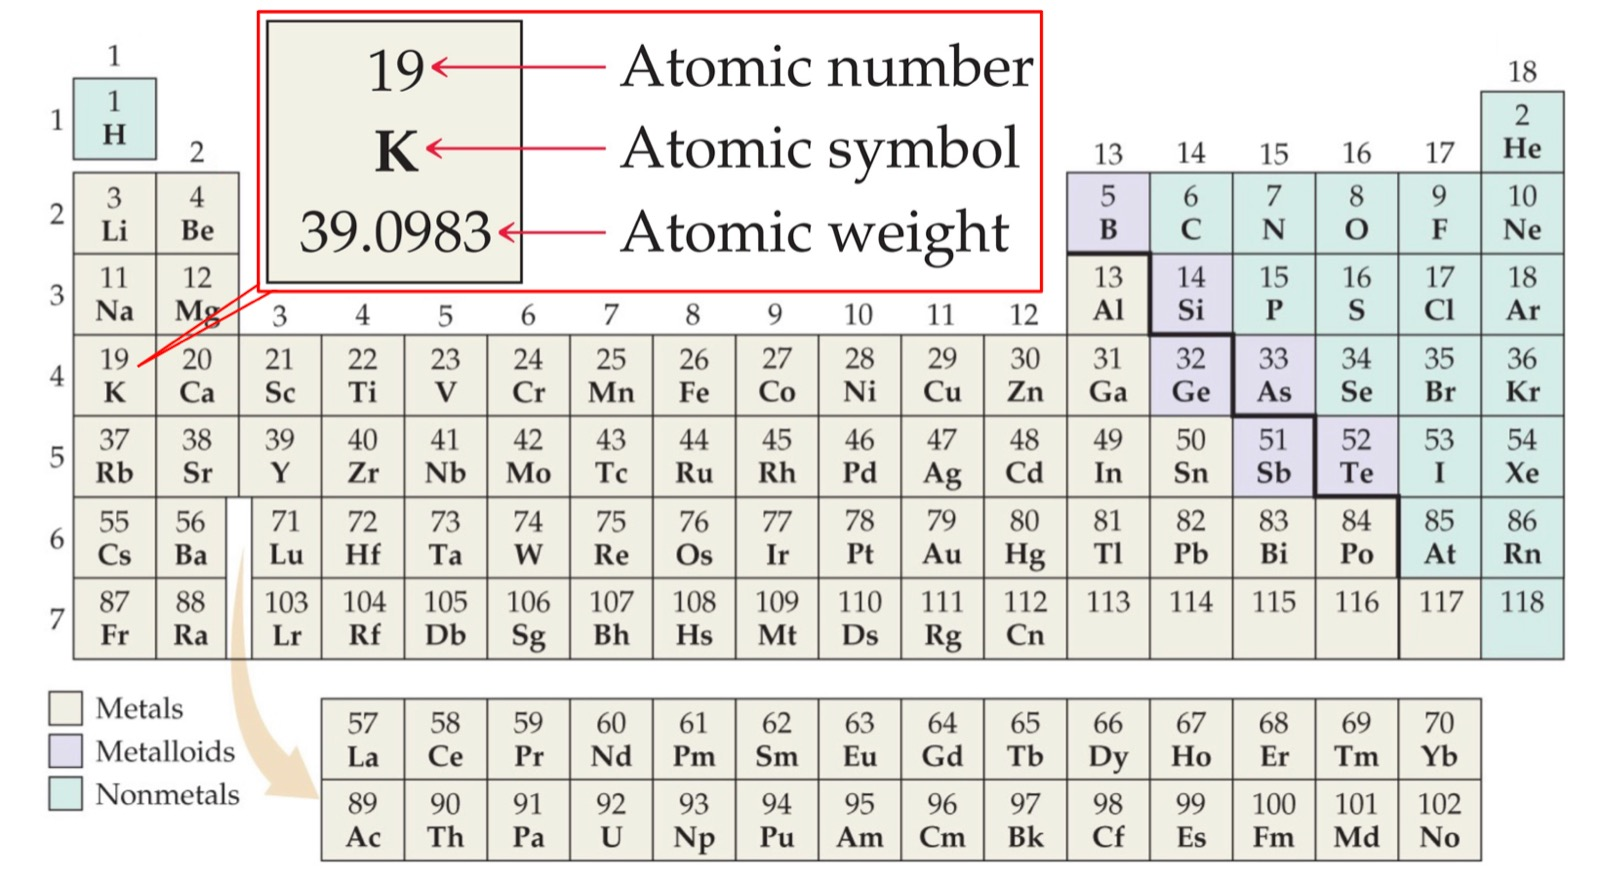
\includegraphics[width = 0.9\linewidth]{images/PSE.jpeg}
        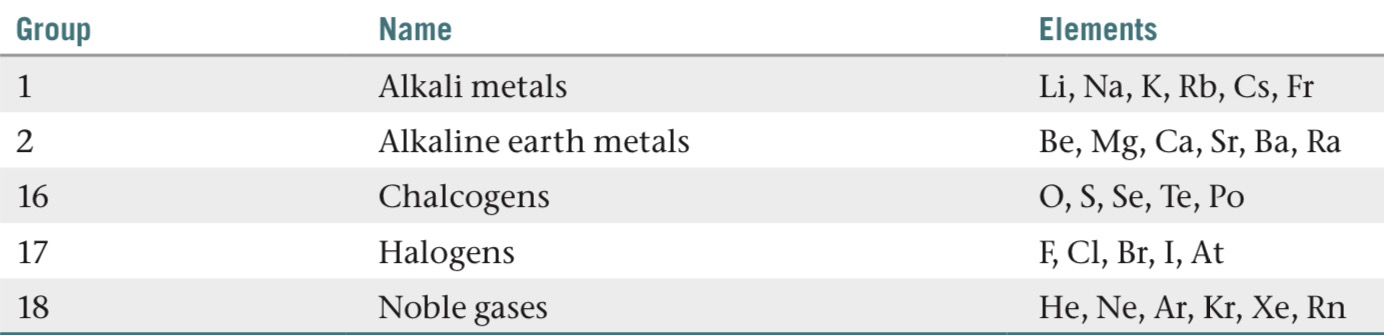
\includegraphics[width = 0.77\linewidth]{images/Groups_PSE.jpeg}
    \end{center}
\end{minipage}
}
\section{Quantum Mechanics}
    \subsection{Basics}
\begin{minipage}{0.15\columnwidth}
\begin{center}
\textbf{Light}\\
\fbox{$ \nu = \frac{c}{\lambda}$} \\
    \textcolor{cyan}{$430nm$}\\
    \textcolor{green}{$530nm$}\\
    \textcolor{red}{$630nm$}\\
\end{center}
  
\end{minipage}
\begin{minipage}{0.20\columnwidth}

\begin{center}
\textbf{Photon Energy}\\
\fbox{$E = h \cdot \nu = h \cdot \frac{c}{\lambda}$}\\
$\nu \equiv$ frequency\\
$c \equiv$ speed of light\\
$\lambda \equiv$ wave length\\
$h \equiv$ Planck's constant 
\end{center}

\end{minipage}
\begin{minipage}{0.25\columnwidth}
\begin{center}
   \textbf{Rydberg Equation}\\ 
   \fbox{$E_H = \frac{hc}{\lambda} = hcR_H(\frac{1}{n_1^2} - \frac{1}{n_2^2})$}\\
   $R_H = 1.097 \cdot 10^7 m^{-1}$
\end{center}
    
\end{minipage}
\begin{minipage}{0.4\columnwidth}
    \begin{center}
        \textbf{Orbital Energies}\\
        \fbox{$E_n = \frac{-hcR_H}{n^2}$} 
        \fbox{$\Delta E = E_{n_f} - E_{n_i} = -hcR_H(\frac{1}{n_f^2} - \frac{1}{n_i^2})$}
        $\Delta E > 0 (n_f > n_i)$: Photon absorbed
        $\Delta E < 0 (n_f < n_i)$: Photon is emitted 
    \end{center}
\end{minipage}
\textcolor{red}{\textbf{Heisenberg's Uncertainty Principle}}\\
\fbox{It is impossible to simultaneously know both the exact momentum of an electron and 
its exact location in space}\\
\fbox{$\Delta x \cdot \Delta (mv) \leq \frac{h}{4 \pi}$} $x \equiv$ position, $mv = p \equiv$ momentum
    \subsection{Orbitals}
\begin{minipage}{0.43\columnwidth}
    \textbf{Orbital Energies}
    \begin{center}
        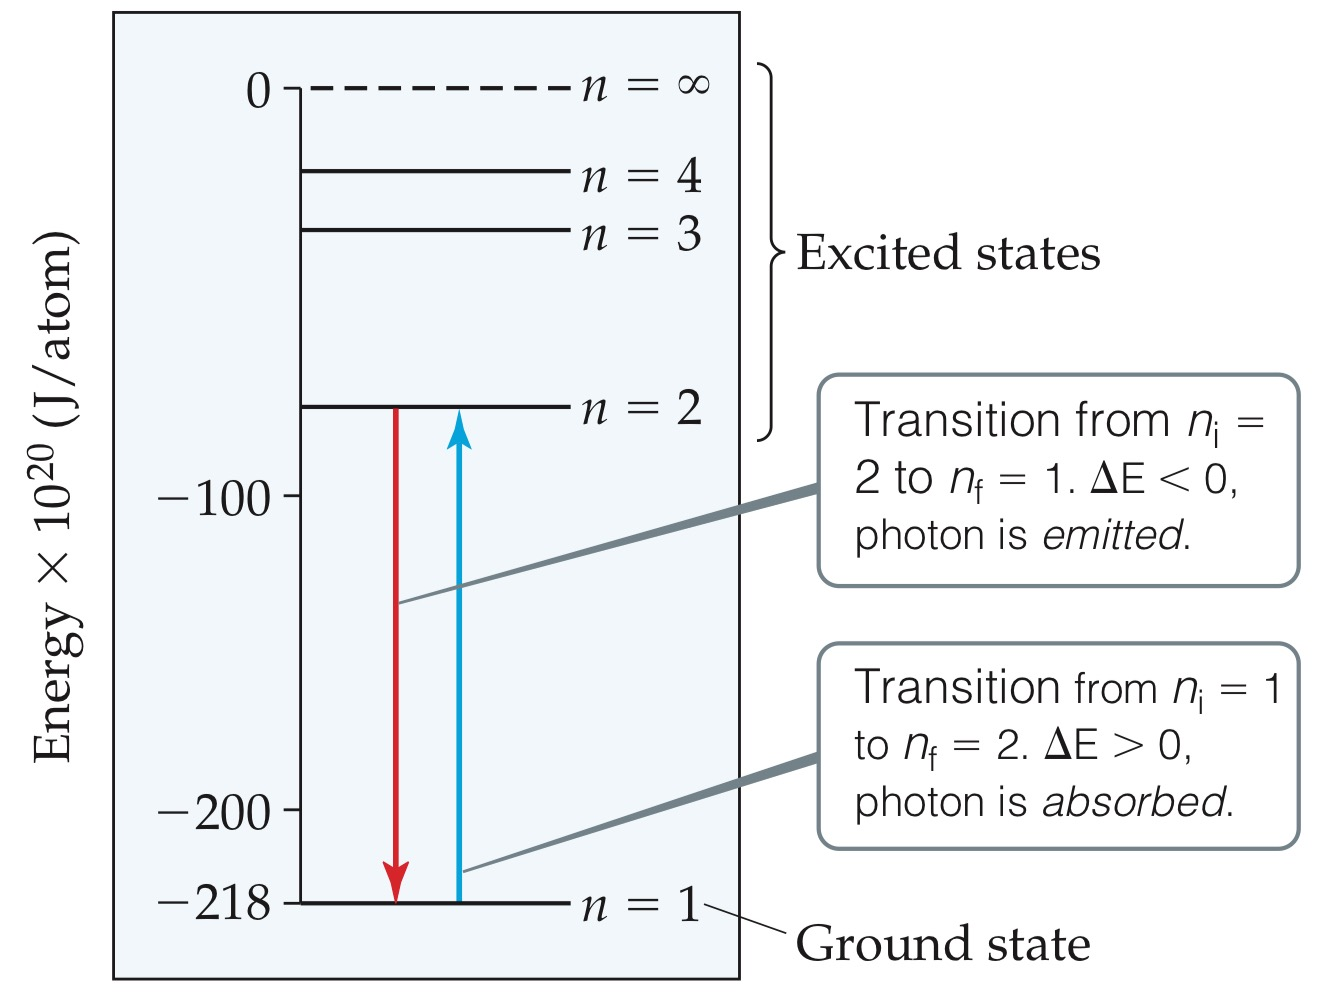
\includegraphics[width = \linewidth]{images/energy_transition_.jpeg}
       
    \end{center}
     \textbf{Quantum Numbers}
    \begin{enumerate}[leftmargin=0.20cm, itemsep=0.05pt]
        \item Principial Quantum Number $n$ (1, 2, 3, ...)
        \item Angular Quantum Number $L$ : [0, n-1],\\
        $0 \equiv$ s, $1 \equiv$ p, $2 \equiv$ d, $3 \equiv$ f
        \item Magnetic quantum Number $m_e$ $[-L, L]$
        \item Spin Magnetic Quantum Number $m_s$ ($-\frac{1}{2}$ or $\frac{1}{2}$)
    \end{enumerate}
    \textcolor{red}{\textbf{Pauli Exclusion Principle}}\\
\fbox{\begin{varwidth}{\textwidth}
\centering
No two electrons in an atom can have the \\ same set of four quantum numbers $n, L, m_e, m_s$
\end{varwidth}}   
 
\end{minipage}
\begin{minipage}{0.56\columnwidth}
    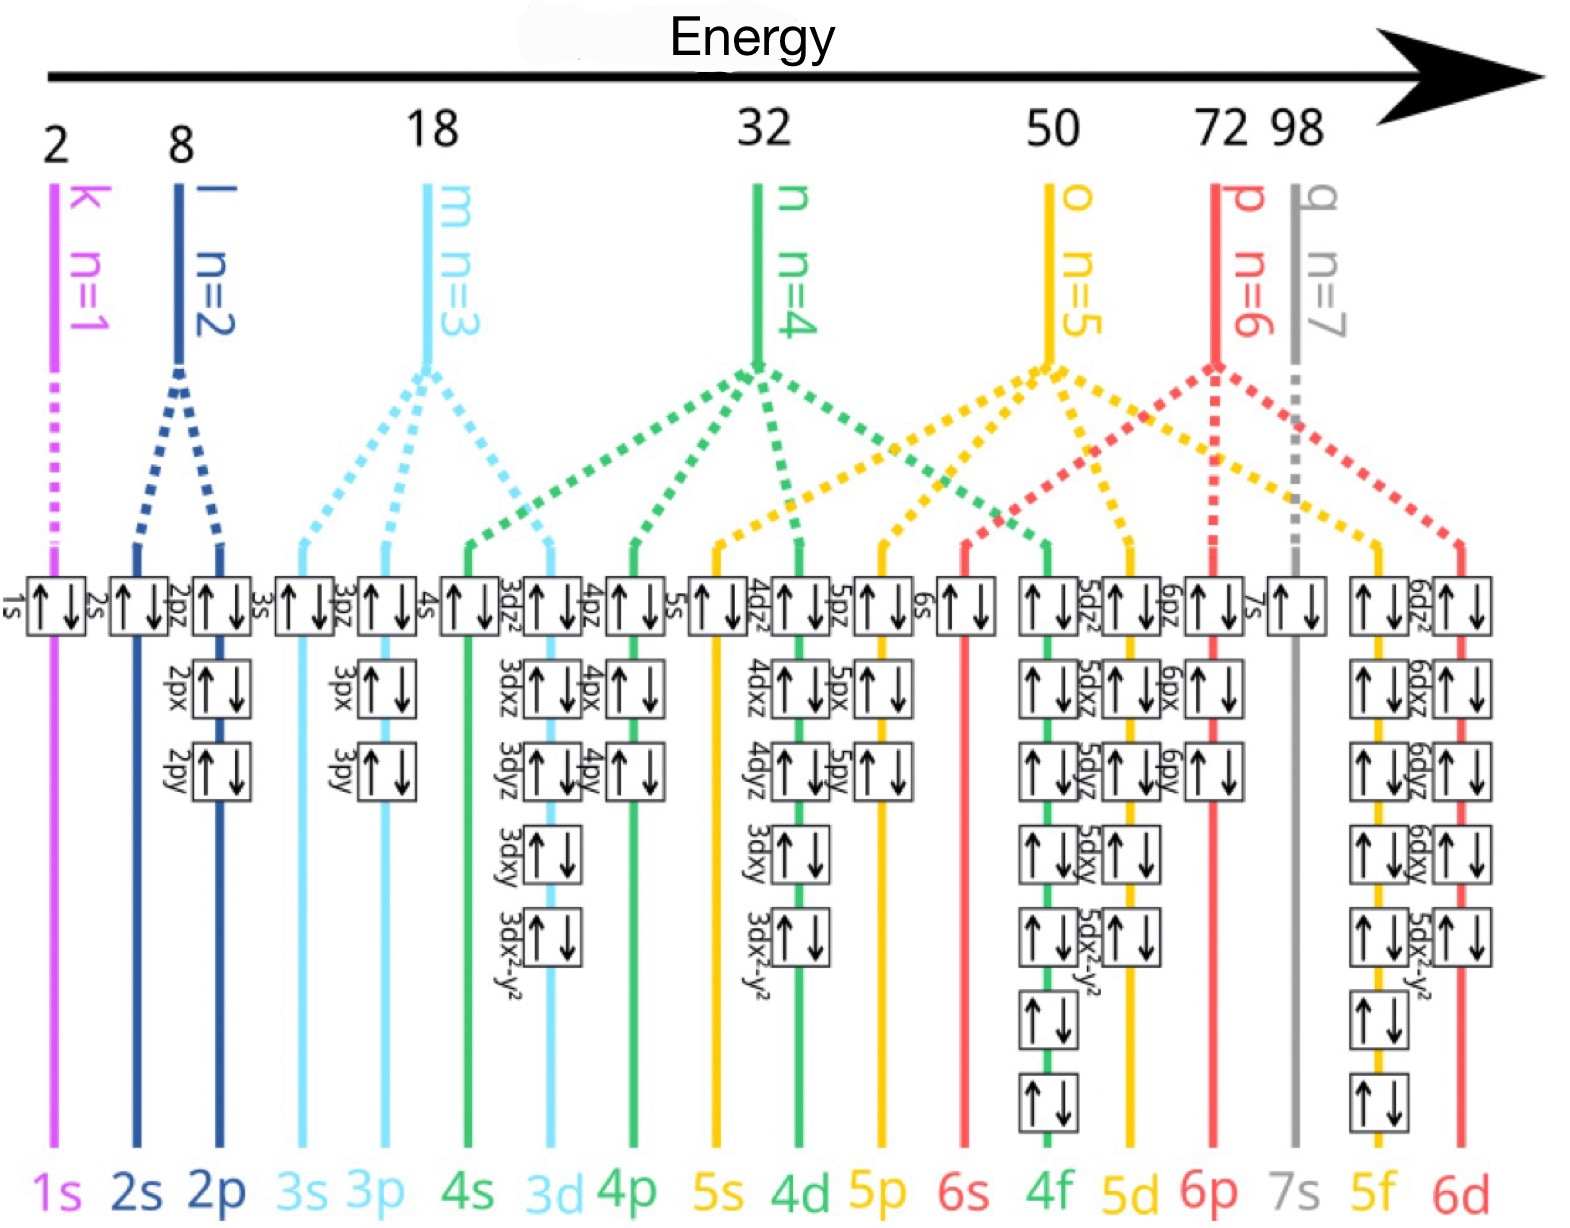
\includegraphics[width = 0.8\linewidth]{images/Orbitals.jpeg}
     \begin{minipage}{0.7\linewidth}
         \begin{center}
             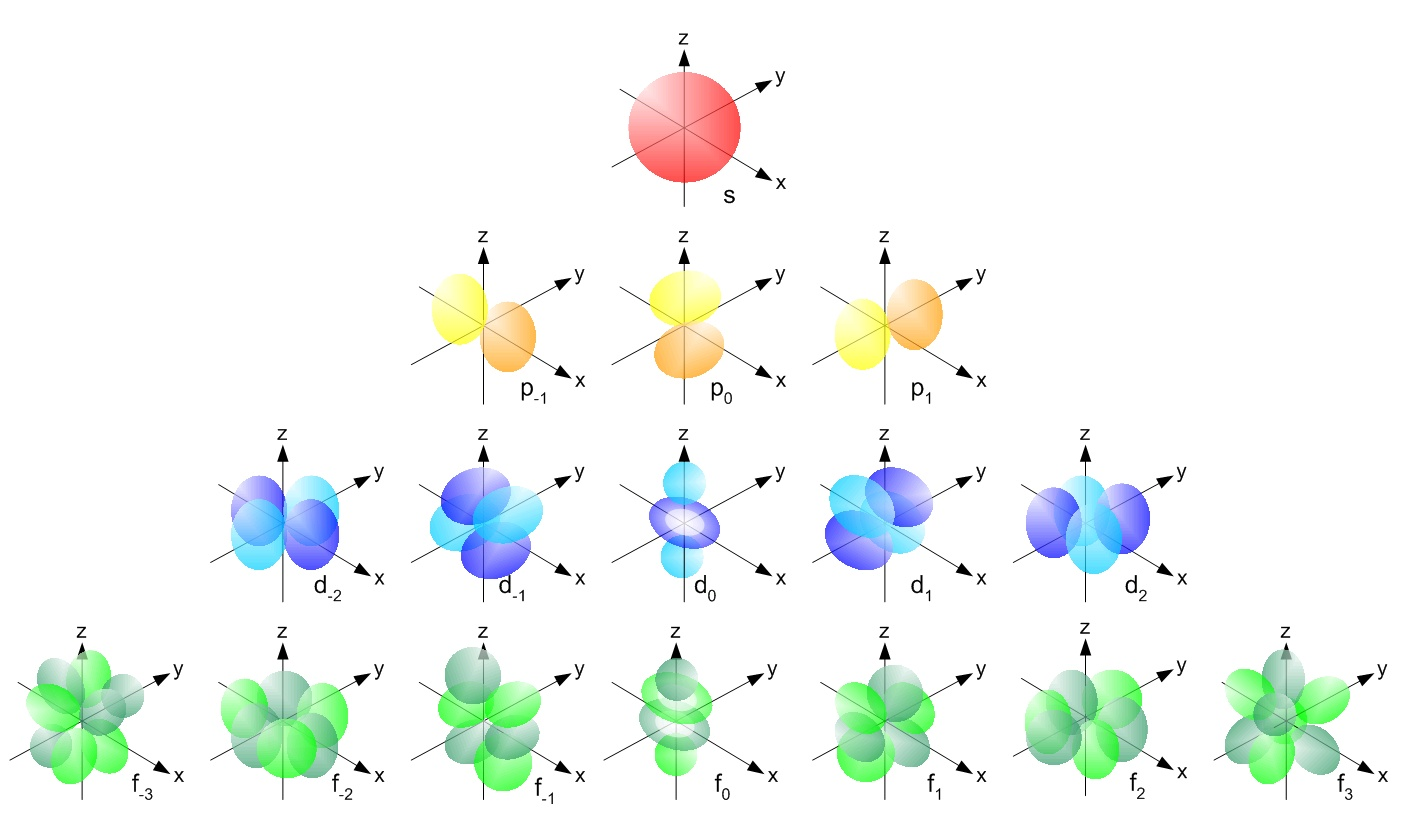
\includegraphics[width = \linewidth]{images/orbital_shapes.jpg}
         \end{center}
     \end{minipage}\\
    \textcolor{red}{\textbf{Hund's Rule}}\\
    \fbox{\begin{varwidth}{\textwidth}
    \centering
    When filling degenerate orbitals the lowest energy is\\ attained when the number of electrons having the same spin is maximized
    \end{varwidth}}  
\end{minipage}

\begin{minipage}{0.60\columnwidth}
    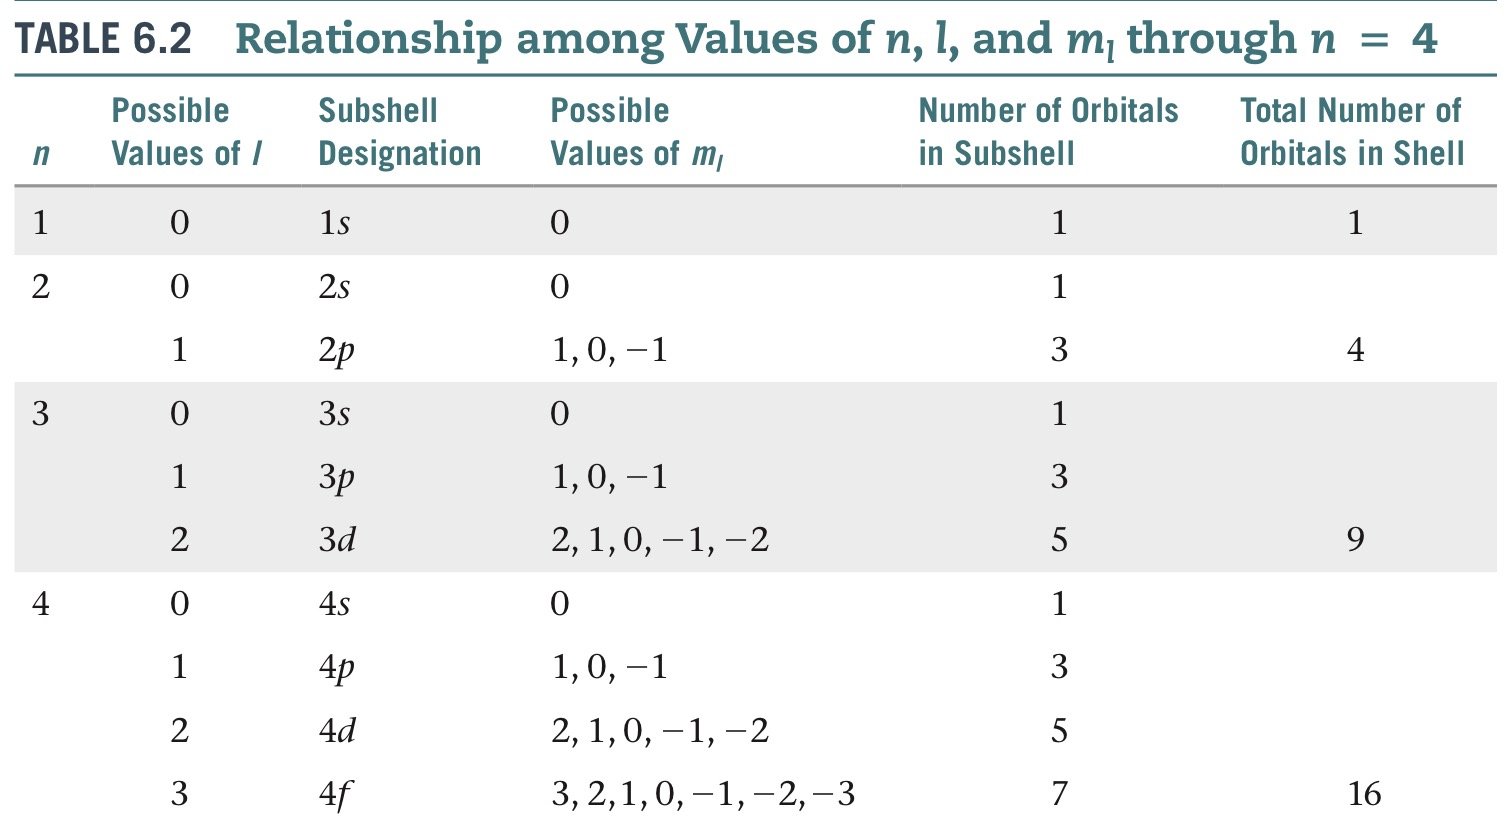
\includegraphics[width = \linewidth]{images/Quantum_numbers_up_to_n_4.jpeg}
\end{minipage}
\begin{minipage}{0.37\columnwidth}
    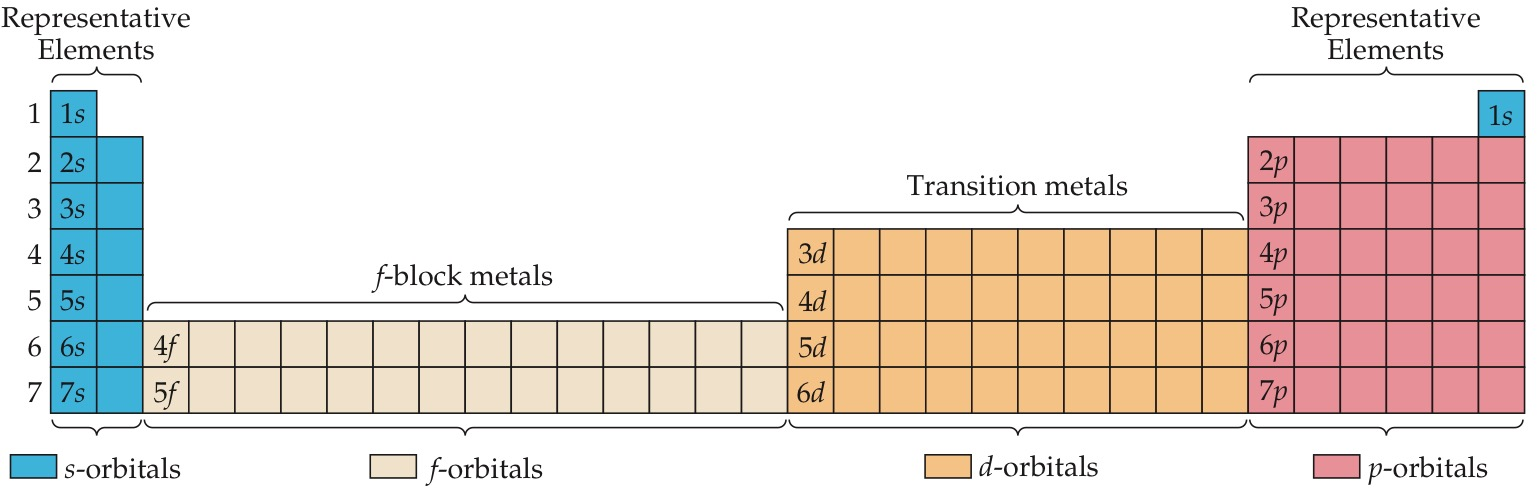
\includegraphics[width = \linewidth]{images/PSE_Quantum_Numbers.jpeg}
    \begin{itemize}
        \item s-orbital: sphere-like
        \item p-orbital: dumbbell-like
        \item d-orbital: usually 4-leafed clover
        \item f-orbital: 2x2 rounded Rubik's cube/other complicated shapes 
    \end{itemize}
\end{minipage}


\section{Chemical Bonds}
    \subsection{Covalent Bonds}
\begin{minipage}{0.49\linewidth}
    \begin{itemize}[leftmargin=0.20cm, itemsep=0.05pt]
        \item Atoms held together by sharing valence electrons
        \item Octet Rule: \# bonds = 8 - \#VE (only strictly applied for groups 1 and 2)
        \item Exceptions: Hypervalence, less than octet, odd number of VE
        \item for H and He: \# bonds = 2 - \#VE
    \end{itemize}
    
\end{minipage}
\begin{minipage}{0.49\linewidth}
    \begin{itemize}[leftmargin=0.20cm, itemsep=0.05pt]
        \item Bond length: triple < double < single
        \item Bond strength: triple > double > single
    \end{itemize}
    \begin{center}
            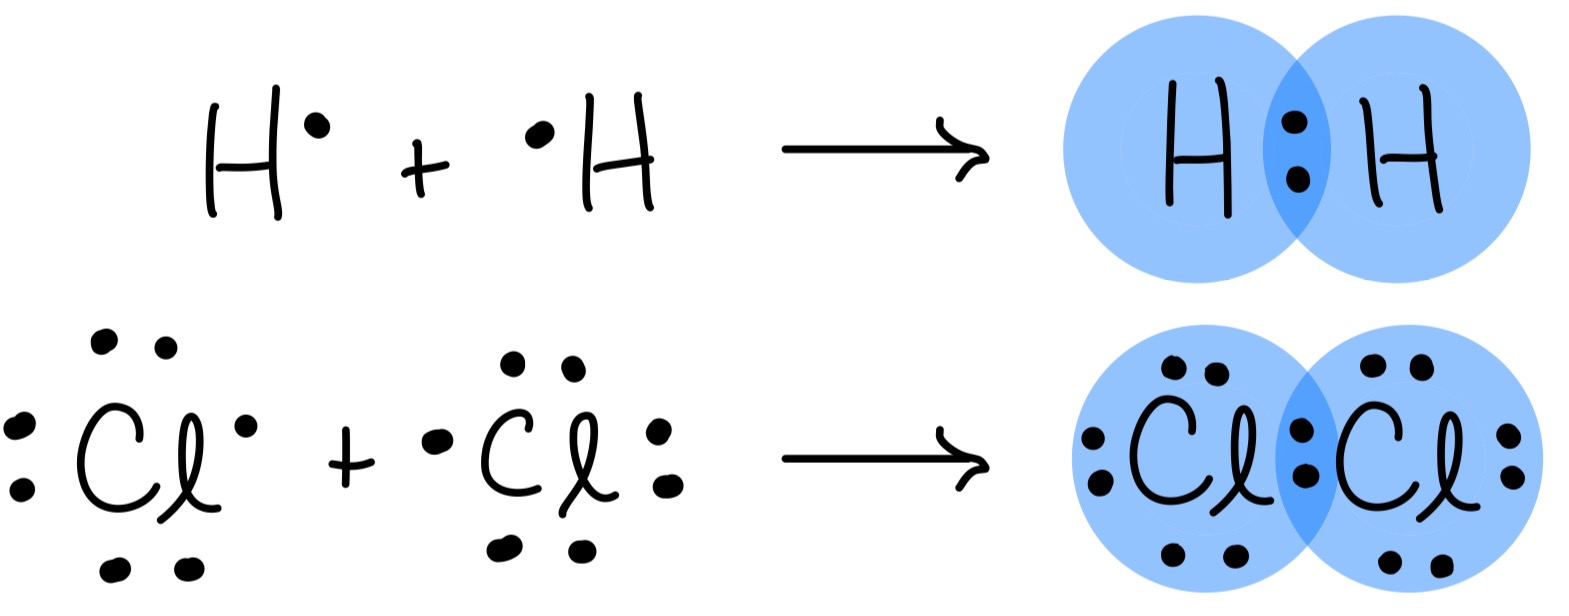
\includegraphics[width = 0.7\linewidth]{images/Covalent_Bonds.jpeg}
    \end{center}
\end{minipage}
    \subsection{Polarity and Dipole Moment}
$\Delta EN < 0.5$: Even distribution of VE, no dipole moment\\
$\Delta EN > 0.5$: Polar bond, partial negative charge at atom with higher electronegativity.\\
$\abs{\vec{\mu}} = Q \cdot r, [\abs{\vec{\mu}}] =$ D (Debye), $1D = 3.34 \cdot 10^{-30} C\cdot m$
\begin{center}
    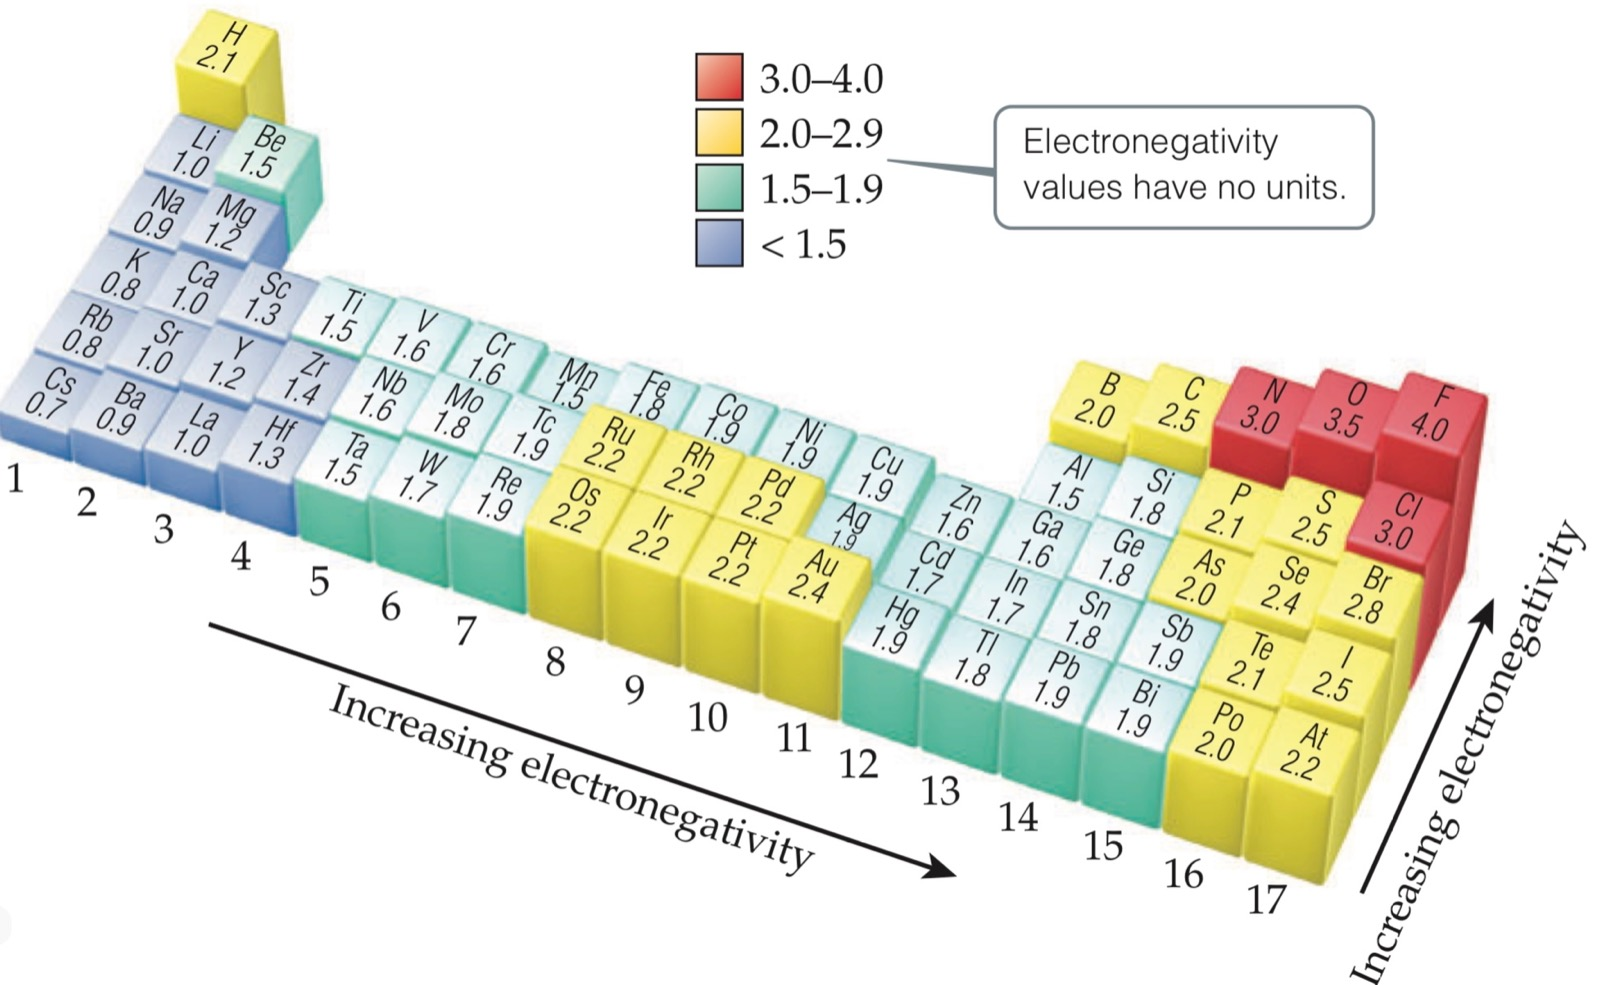
\includegraphics[width = 0.8\linewidth]{images/electronegativity.jpeg}
\end{center}

    \subsection{Lewis Structure}
\begin{minipage}{0.49\linewidth}
 \textbf{Drawing Lewis Structures}\\
1. Sum VE of all atoms\\
2. Write symbols and connect with single bonds\\
3. Complete octets around non-central atoms\\
4. Place remaining VE around central atom\\
5. Try multiple bonds if central atom does not have octet\\
\vspace{3pt}\\
\textbf{Alternative Lewis Structure}\\
$\circ$ More than one Lewis Structure possible\\
$\circ$ Calculate formal charges of each atom\\
$\circ$ Formal charges closest to zero with negative formal charges on more EN atoms is dominant\\
$\circ$ A molecule is most stable when it has the least overall formal charge\\
\fbox{Formal Charge $=$ Atom's VE $- \frac{1}{2}$ (Atom's bonding e's) $-$ (Atom's non-bonding e's)}
\end{minipage}
\begin{minipage}{0.24\linewidth}
      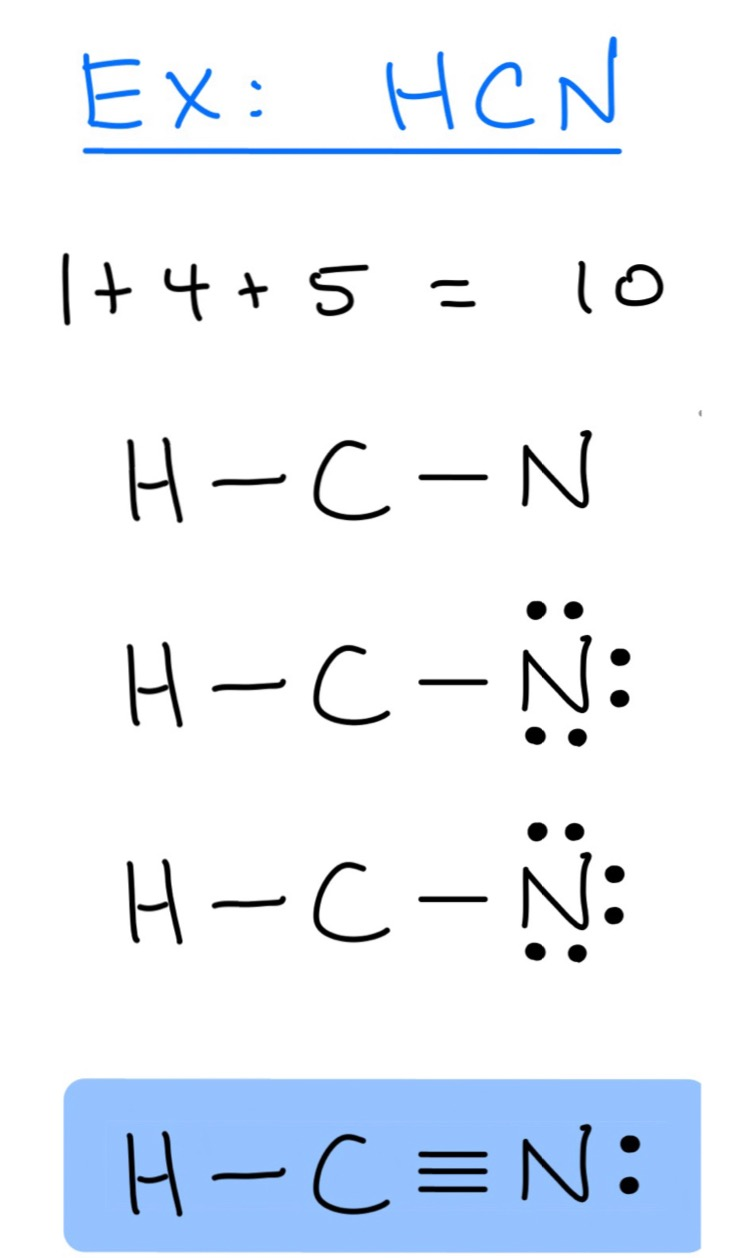
\includegraphics[width = 0.6\linewidth]{images/Lewis_Structure_HCN.jpeg}
      \\
      \\
\end{minipage}
\begin{minipage}{0.24\linewidth}
    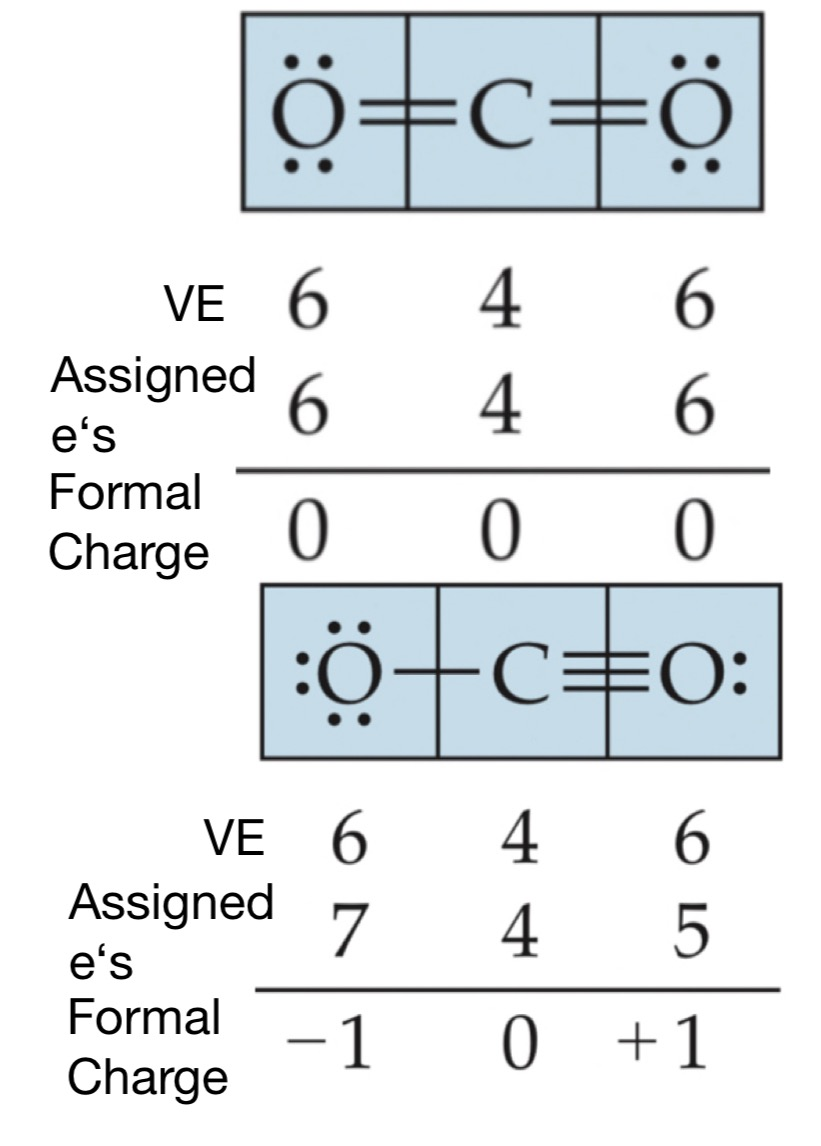
\includegraphics[width = \linewidth]{images/Lewis_Structure_CO2.jpeg}
\end{minipage}


    \subsection{Ionic Bond}
\begin{minipage}{0.55\linewidth}
    $\circ$ Ions held together by electrostatic attraction\\
    $\circ$ Metal loses VE, non-metal gains VE\\
    $\circ$ Strength quantified by lattice energy\\
    $\circ$ Bond is considered ionic if $\Delta EN > 2.0$\\
    \vspace{1pt}\\
    \textbf{Some Definitions}\\
    \textbf{Ionization Energy}: energy required to ionize (remove) $e^-$ from atom or ion\\
    \textbf{Electron Affinity}: energy change when adding and extra $e^-$ to an atom (typically exothermic)\\
    \textbf{Lattice Energy}: energy required to separate ions in ionic solid to infinite distance 
\end{minipage}
\begin{minipage}{0.44\linewidth}
    \begin{center}
        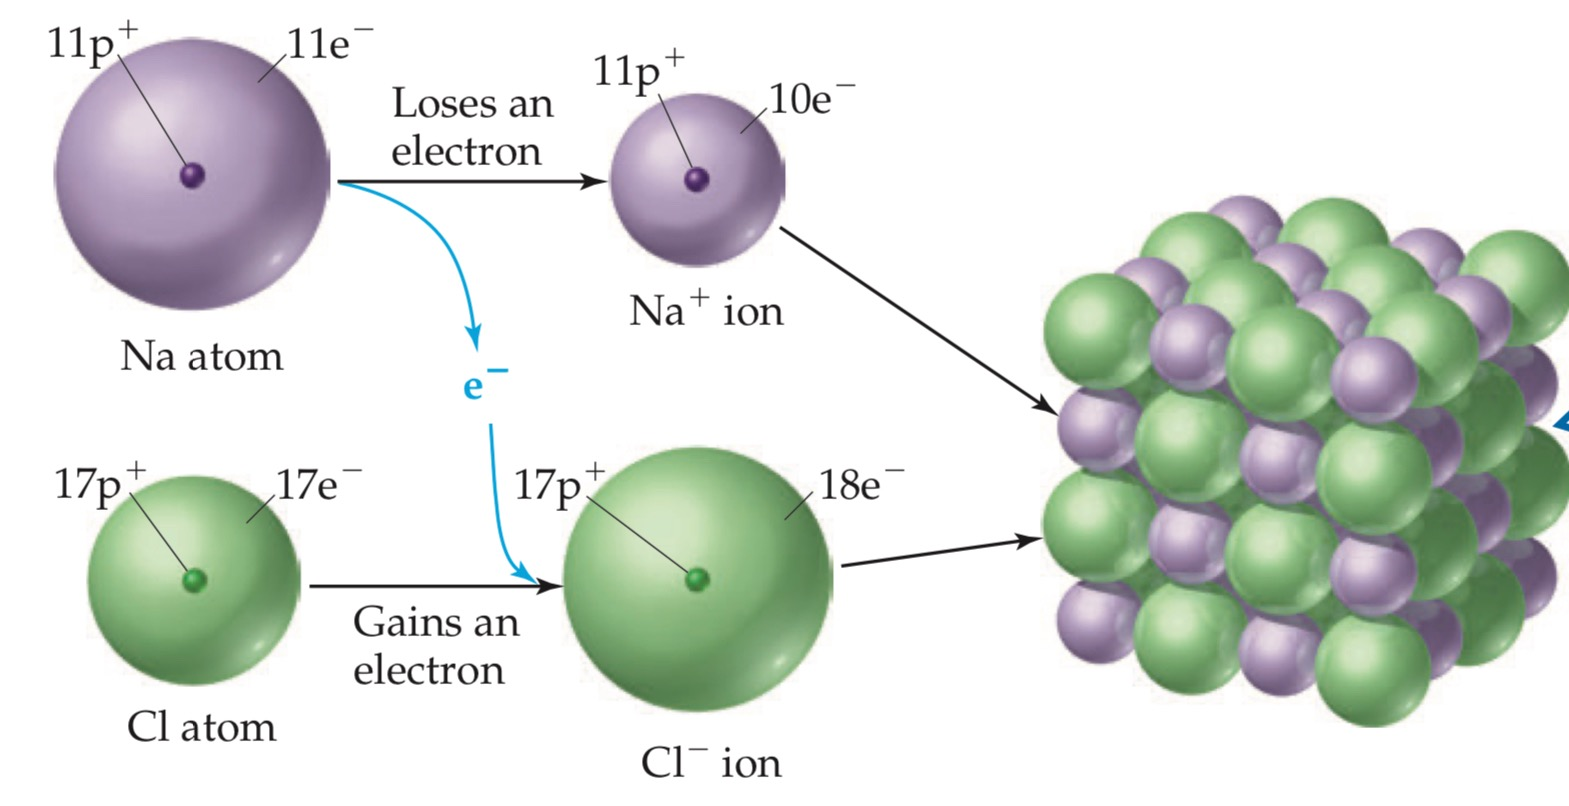
\includegraphics[width = 0.9\linewidth]{images/NaCl.jpeg}
    \end{center}
\end{minipage}\\
\vspace{1pt}\\
\textbf{Bookkeeping Systems}\\
\begin{center}
  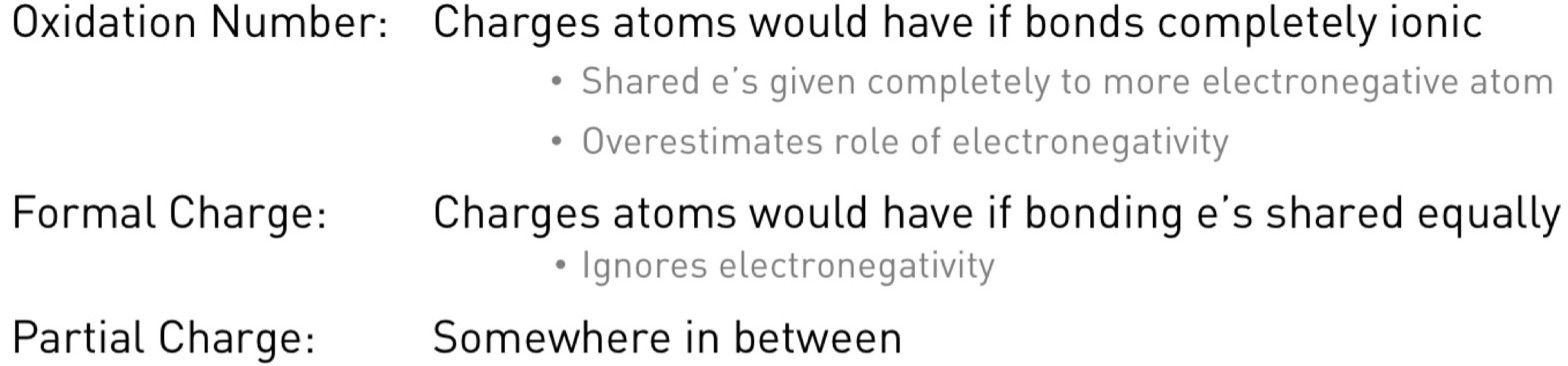
\includegraphics[width = 0.7\linewidth]{images/Bookkeeping_Systems.jpeg} 
\end{center}
\textbf{Oxidation Numbers}\\
\begin{center}
  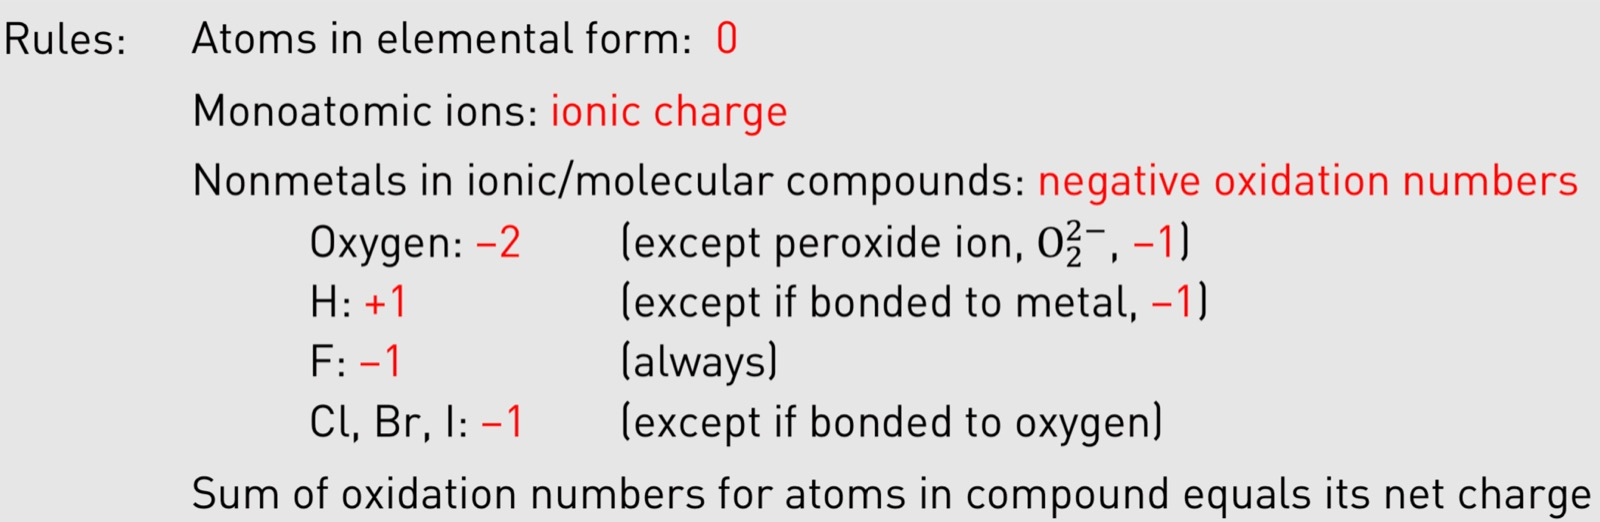
\includegraphics[width = 0.95\linewidth]{images/Oxidations_Numbers.jpeg} 
\end{center}
\textbf{Lattice Energy (e.g NaCl)}\\
\begin{minipage}{0.6\linewidth}
\begin{center}
   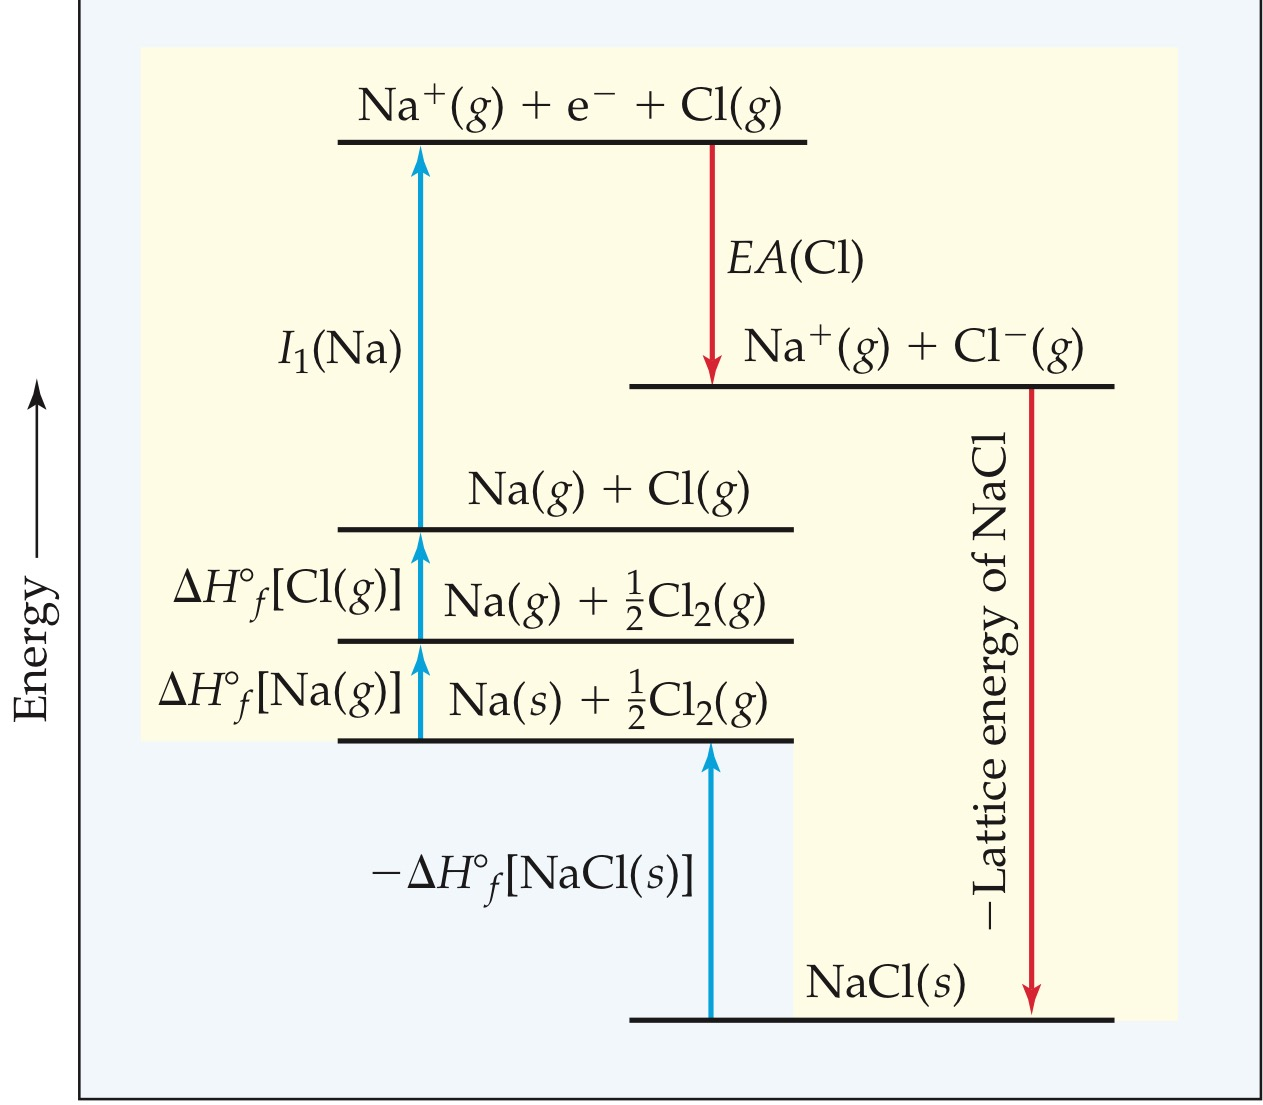
\includegraphics[width = 0.8\linewidth]{images/Lattice_Energy_NaCl.jpeg}     
\end{center}

\end{minipage}
\begin{minipage}{0.39\linewidth}
\begin{center}
    {\normalsize $\Delta H_{lattice}$ \\
    $= - \Delta H_f^{\circ}[NaCl(s)]$ \\
    $+ \Delta H_f^{\circ}[Na(g)]$\\
    $+ \Delta H_f^{\circ}[Cl(g)]$\\
    $+ I_1[Na]$\\
    $+ EA[Cl]$}
\end{center}
   
\end{minipage}


    \subsection{Metallic Bond}
\begin{minipage}{0.4\linewidth}
    \begin{center}
        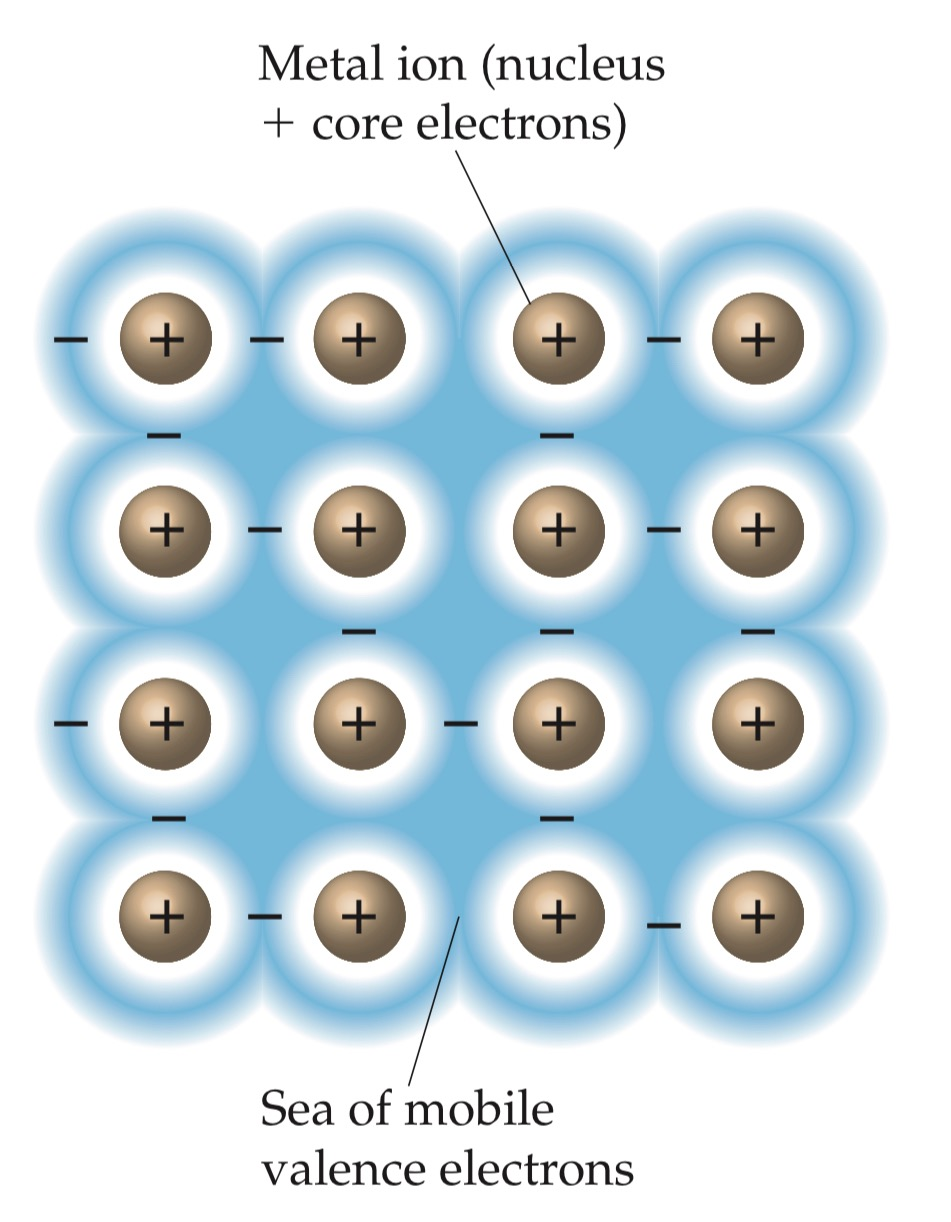
\includegraphics[width = 0.7\linewidth]{images/Metallic_Bond.jpeg}
    \end{center}
\end{minipage}
\begin{minipage}{0.59\linewidth}
\begin{itemize}[leftmargin=0.20cm, itemsep=0.05pt]
    \item VE shared with entire solid
    \item Positive core surrounded by negatively charge electron cloud
    \item  Metals have a deficit of VE and therefore do not form covalent bonds
    \item Freely movable electron cloud is cause for high thermal and electrical conductivity
\end{itemize}
\end{minipage}
\section{Molecule Models}
    \subsection{VSEPR}
1. Draw Lewis structure\\
2. Count electron domains\\
3. Determine electron domain geometry\\
4. Determine molecular geometry from position of atoms
\begin{center}
  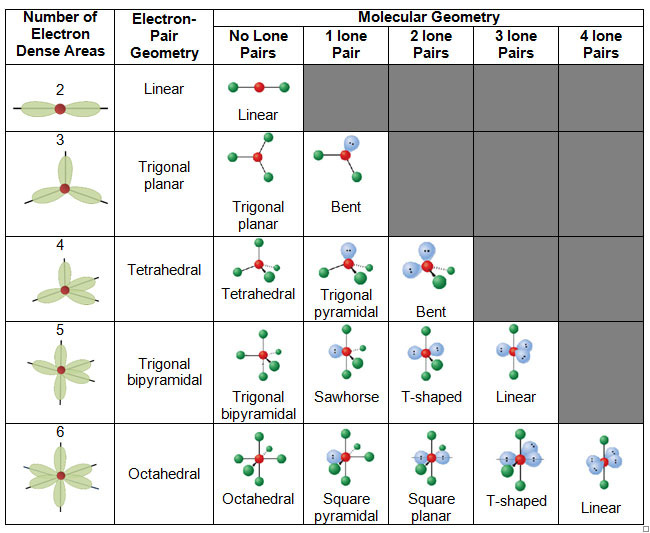
\includegraphics[width = 0.88 \linewidth]{images/VSEPR_model.jpg}  
\end{center}

\section{Aggregate States}
    \subsection{5.1 Intermolecular Forces}
1. \textbf{Van der Waals Forces (weak)}:\\
a. \textbf{London Dispersion Force}: Instantaneous charge fluctuations leading to repelling and attraction between atoms (always present). Big and long molecules have high dispersion\\
b. \textbf{Dipole-Dipole}: Sum of all dipole moments from polarbonds $\longrightarrow$ molecular dipole (present in polar molecules)\\
\vspace{1pt}\\
2. \textbf{Hydrogen Bonding (substantial)}:\\
Occurs between N, O, F atoms and H, which is attracted to unbonded e's of highly EN atoms\\
\vspace{1pt}\\
3. \textbf{Ion-Dipole Interactions}: Dipoles of polar molecules orient themselves with positive and negative ions (present in ionic solid dissolved in polar liquids)\\
\vspace{1pt}\\
\textbf{Strength}: London Dispersion Force $\simeq$ Dipole-Dipole < H-Bonding < Ion-Dipole
    \subsection{Liquids}
\textbf{Properites of Liquids}\\
1. \textbf{Viscosity}: Resistance to flow. Internal friction of liquid molecules, which slows flow.\\
\vspace{1pt}\\
2. \textbf{Surface Tension}: Energy per unit area of liquid surface. Tendency for liquid surfaces at rest to shrink to the minimal surface area possible.\\
\vspace{1pt}\\
3. \textbf{Vapor Pressure}: Pressure of molecules in gas phase. Dynamics Equilibrium between molecules leaving/entering gas phase, which has to be reestablished when $T$ changes. \\
\begin{minipage}{0.45\linewidth}
    \textbf{Clausius-Clapeyron Equation}\\
    \fbox{$ln(P) ) \frac{-\Delta H_{vap}}{RT} + C$}\\
    \fbox{$ln(\frac{P_1}{P_2} = \frac{-\Delta H_{vap}}{R}(\frac{1}{T_1} - \frac{1}{T_2})$}\\
    \begin{center}
        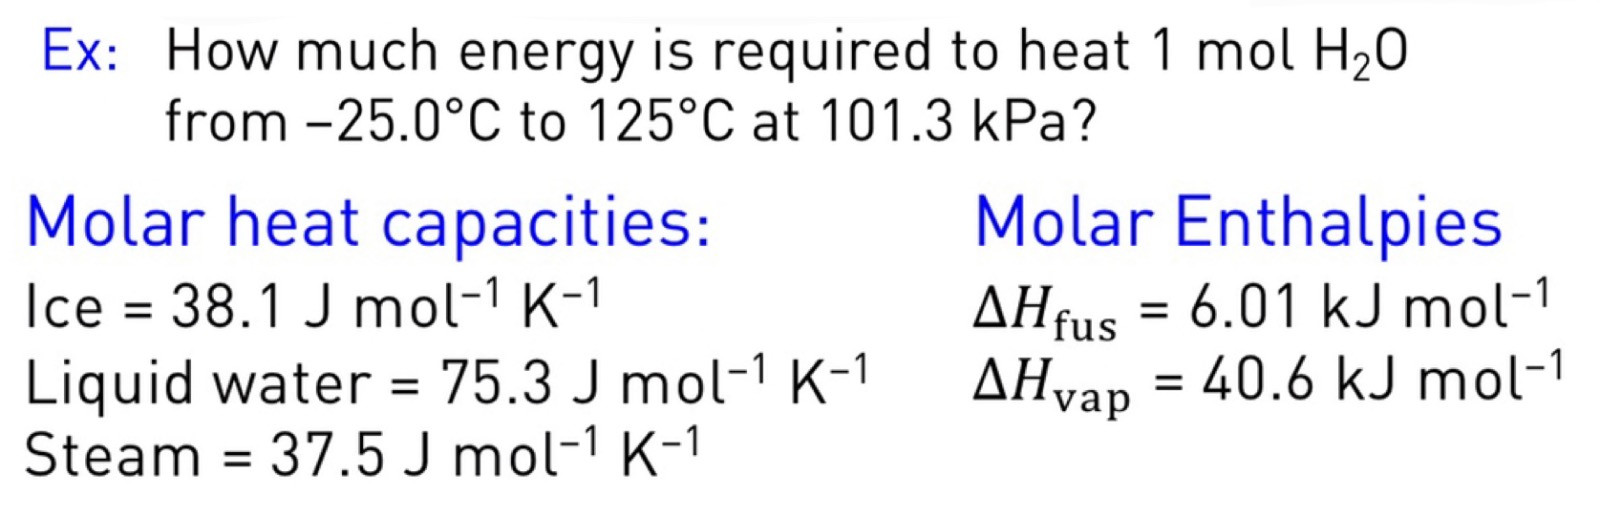
\includegraphics[width = \linewidth]{images/heating process example.jpeg}
    \end{center}
\end{minipage}
\begin{minipage}{0.27\linewidth}
    \begin{center}
        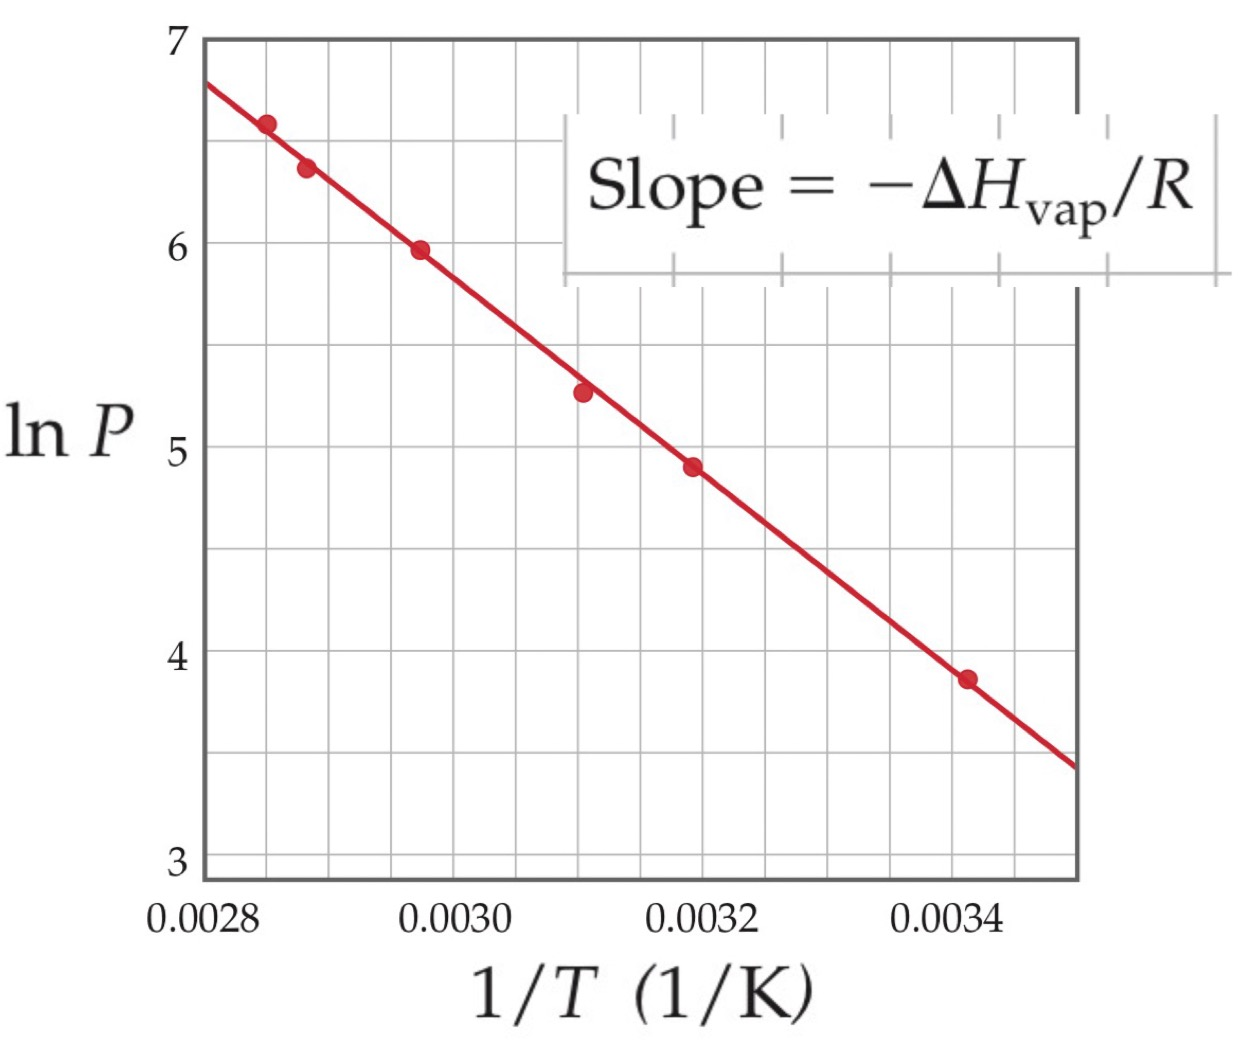
\includegraphics[width = \linewidth]{images/Clausius-Clapyeron.jpeg}
       
    \end{center}
\end{minipage}
\begin{minipage}{0.27\linewidth}
\begin{center}
\textbf{Heating Curves}
   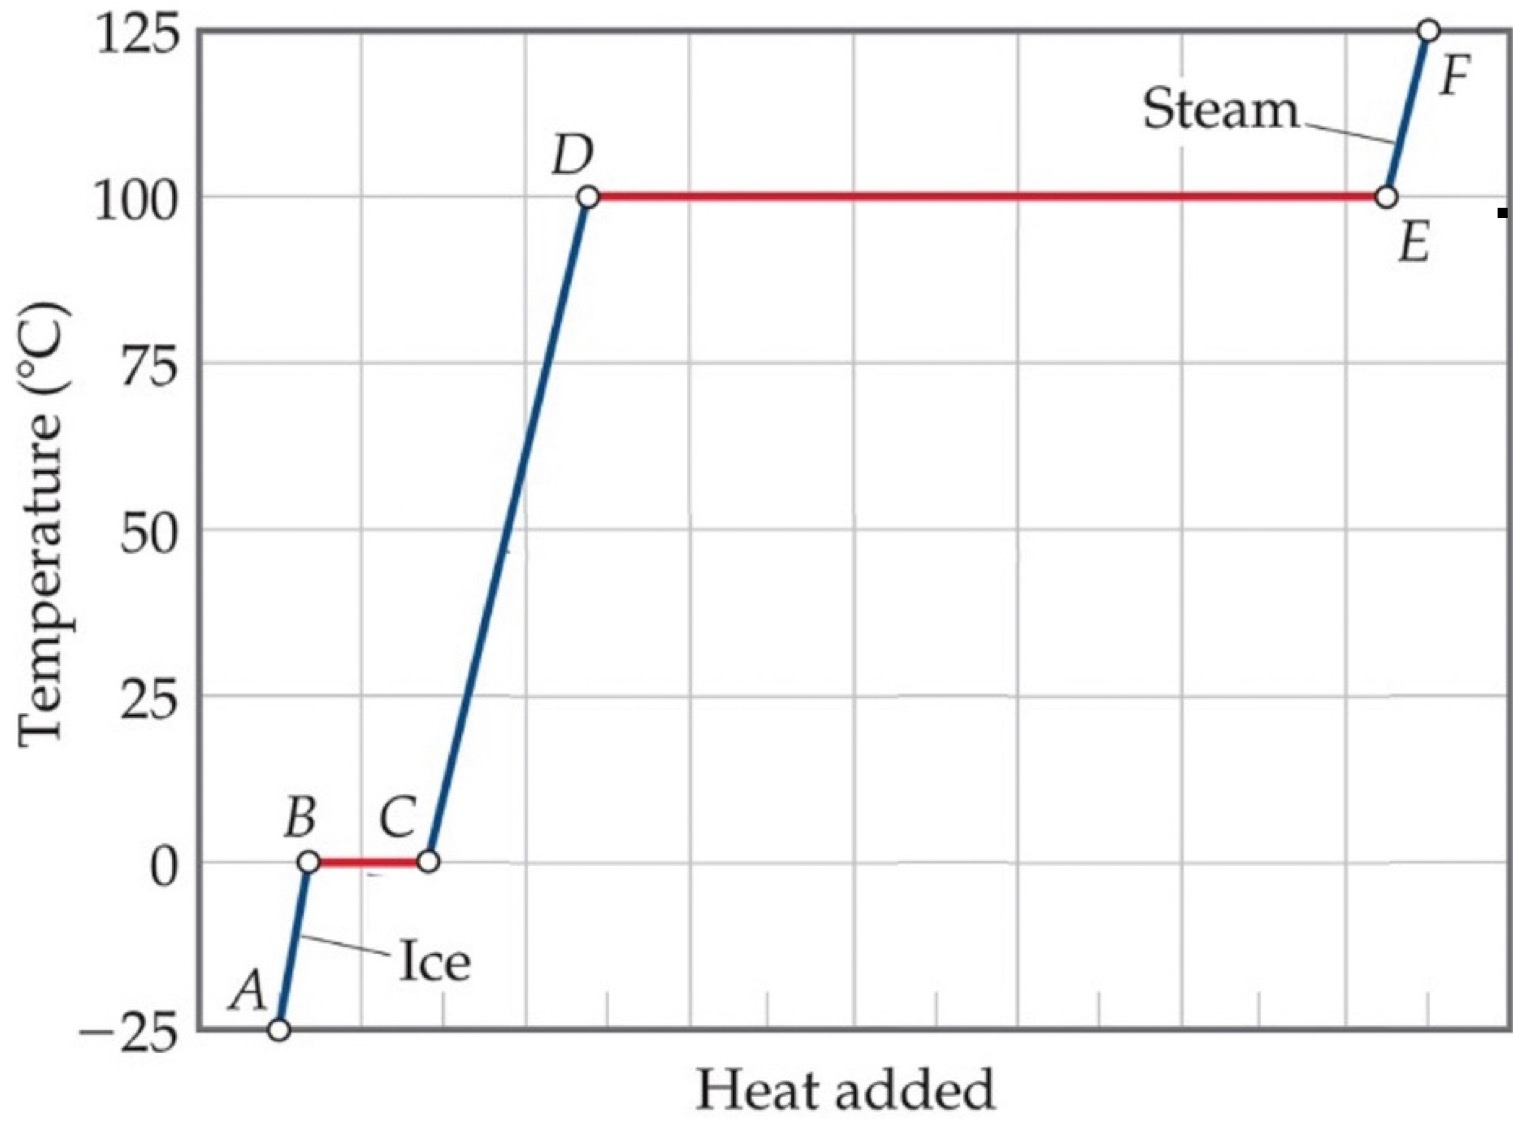
\includegraphics[width = \linewidth]{images/Heating_curve.jpeg} 
    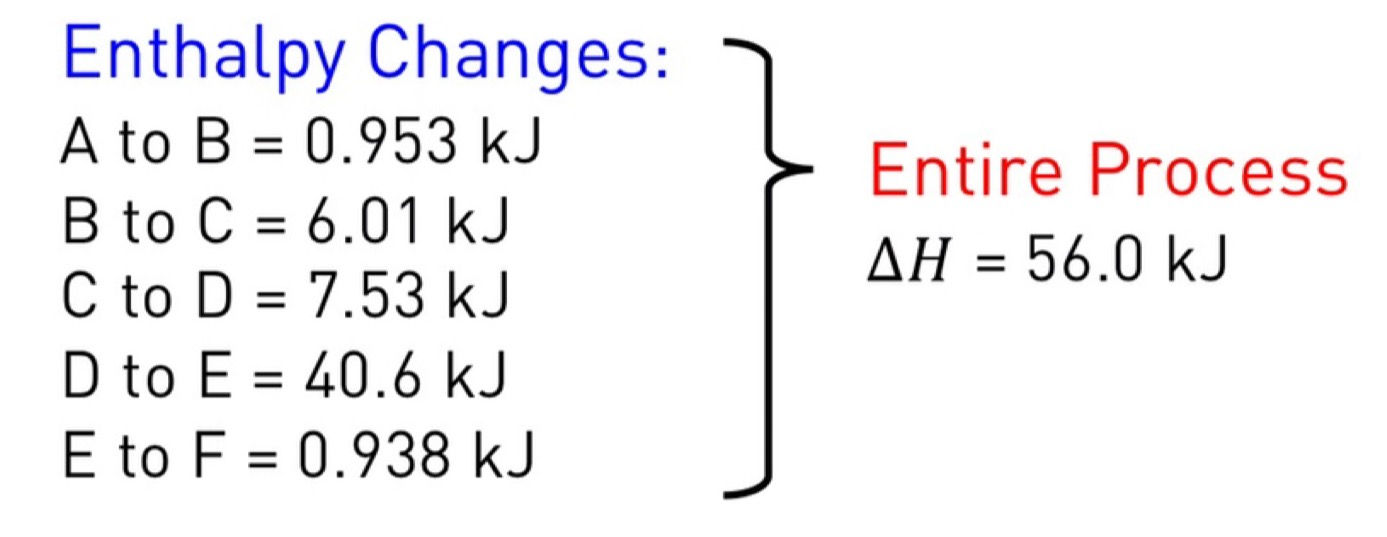
\includegraphics[width = \linewidth]{images/Heating_curve_2.jpeg}
\end{center}
    
\end{minipage}

\begin{minipage}{0.6\linewidth}
    \begin{center}
        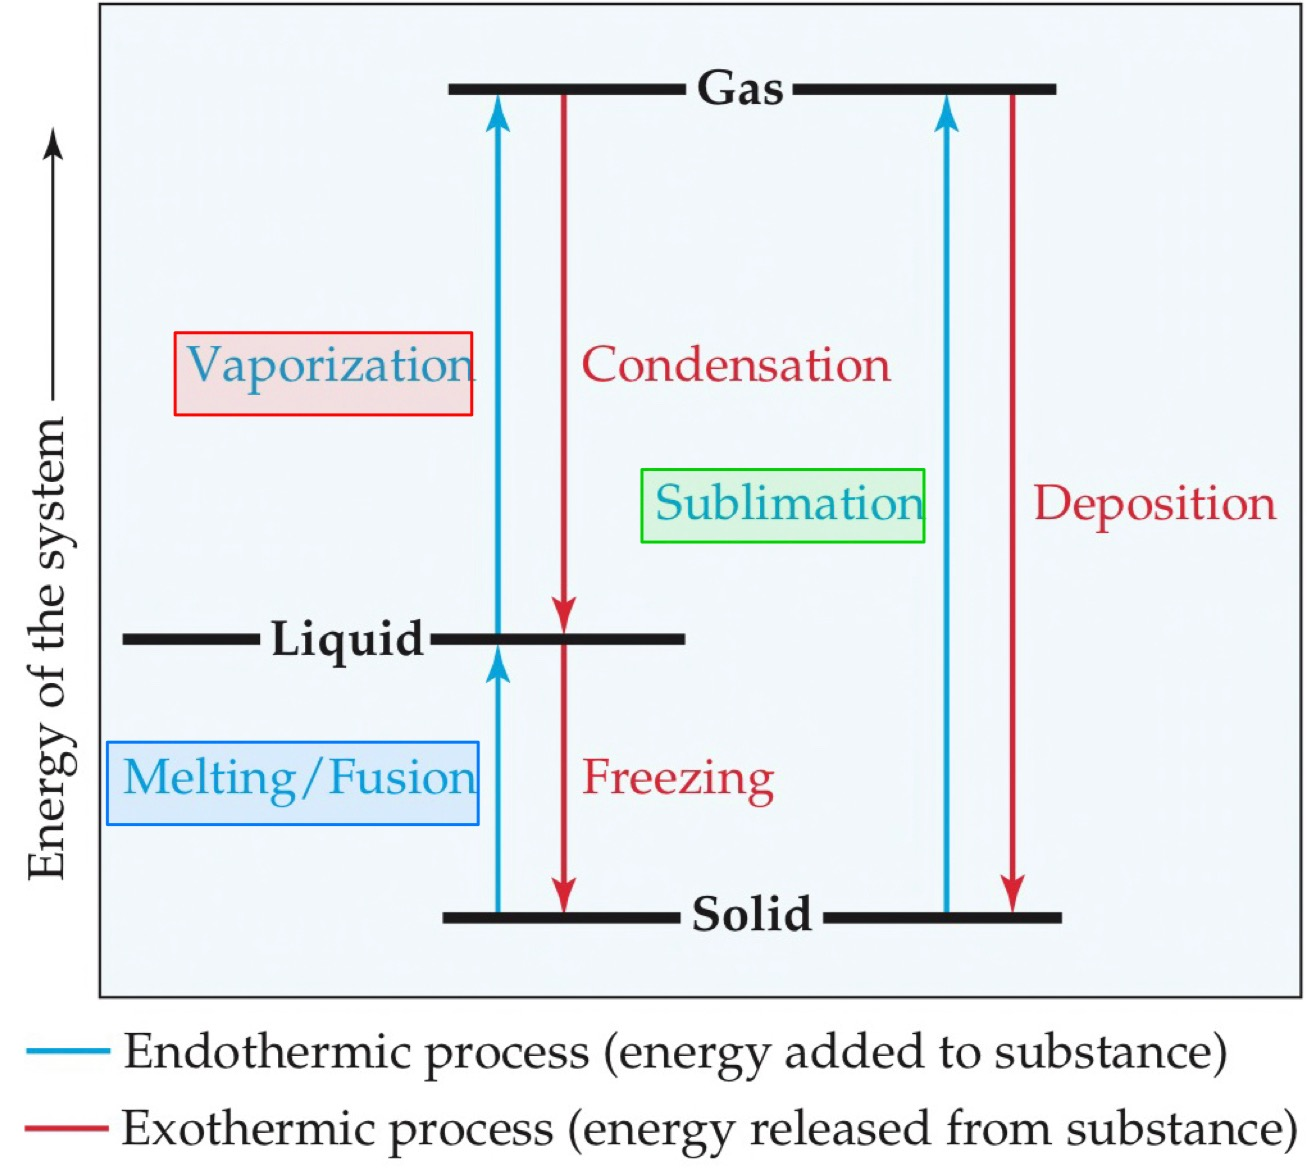
\includegraphics[width = 0.8\linewidth]{images/Water_changes_agg_state.jpeg}
    \end{center}
\end{minipage}
\begin{minipage}{0.39\linewidth}
    \begin{center}
    {\small 
        \textcolor{blue}{$\Delta H_{fus} \equiv$ Heat of fusion}
        \vspace{3pt}\\
        \textcolor{red}{$\Delta H_{vap} \equiv$ Heat of vaporization}
        \vspace{3pt}\\
        \textcolor{green}{$\Delta H_{sub} \equiv$ Heat of sublimation}
        \vspace{3pt}\\
        \textcolor{green}{$\Delta H_{sub}$} $=$ \textcolor{blue}{$\Delta H_{fus}$} $+$  \textcolor{red}{$\Delta H_{vap}$}
        \vspace{3pt}\\
        \textcolor{red}{$\Delta H_{vap}$} $>$ \textcolor{blue}{$\Delta H_{fus}$}
        }
    \end{center}
\end{minipage}
\begin{center}
    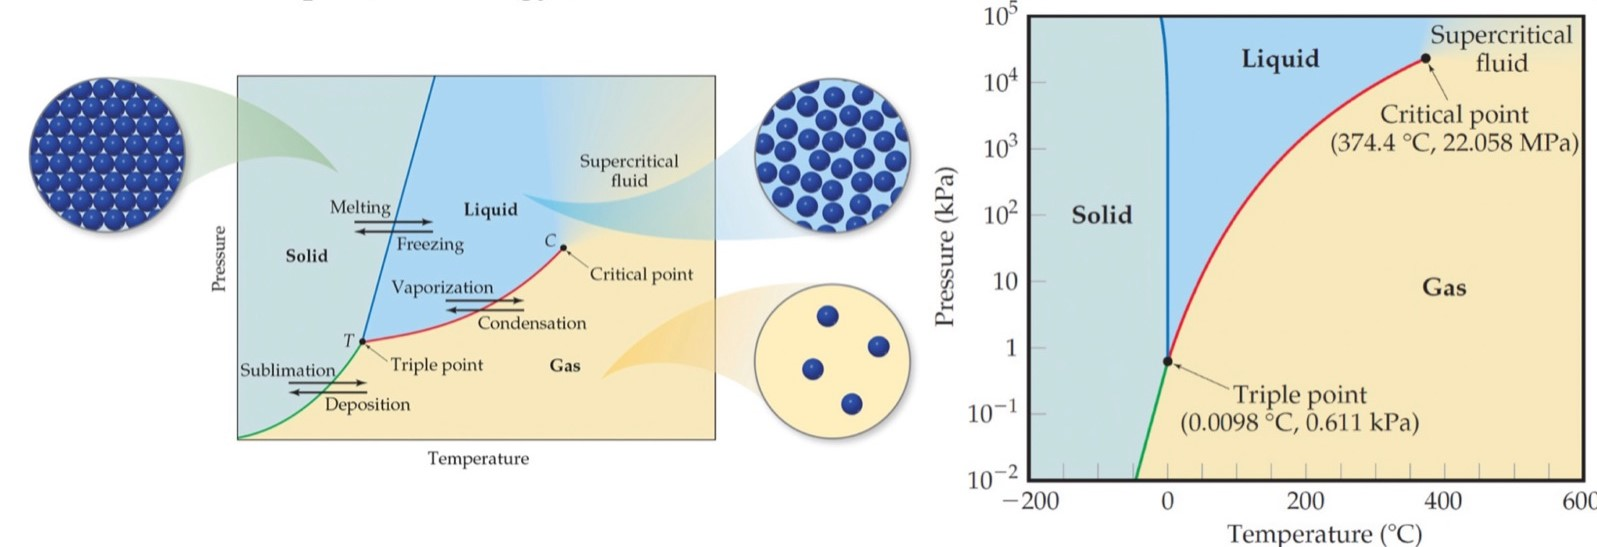
\includegraphics[width = 0.9\linewidth]{images/PvsT_water.jpeg}
\end{center}
    \subsection{Solutions and Colligative Properties}
\textbf{Solution}: Homogeneous mixture of two ro more substances \hspace{3pt}
\fbox{solution $=$ solvent $+$ solute(s)}\\

\textbf{Precipitation Reaction}: Reactions that result in the formation of an insoluable product are called precipitation reactions.\\
\textbf{e.g.} $Ag(NO_3)(aq) + KCl(aq) \longrightarrow AgCl(s) + KNO_3 (aq)$ \hspace{3pt} $AgCl$ is the solid precipitate\\

\textbf{Ionic Equations}\\
\textbf{1. Comple Ionic eq.} \textbf{e.g.}$Ag^{+}(aq) + NO_3^{-}(aq) + K^{+}(aq) + Cl^{-}(aq) \longrightarrow AgCl(s) + K^{+}(aq) + NO_3^{-}$\\
$K^{+}(aq)$ and $NO_3^{-}(aq)$ are spectator ions\\
\textbf{2. Net Ionic eq.} \textbf{e.g.} $Ag^{+}(aq) + Cl^{-}(aq) \longrightarrow AgCl(s)$

\begin{minipage}{0.6\linewidth}
    \begin{center}
        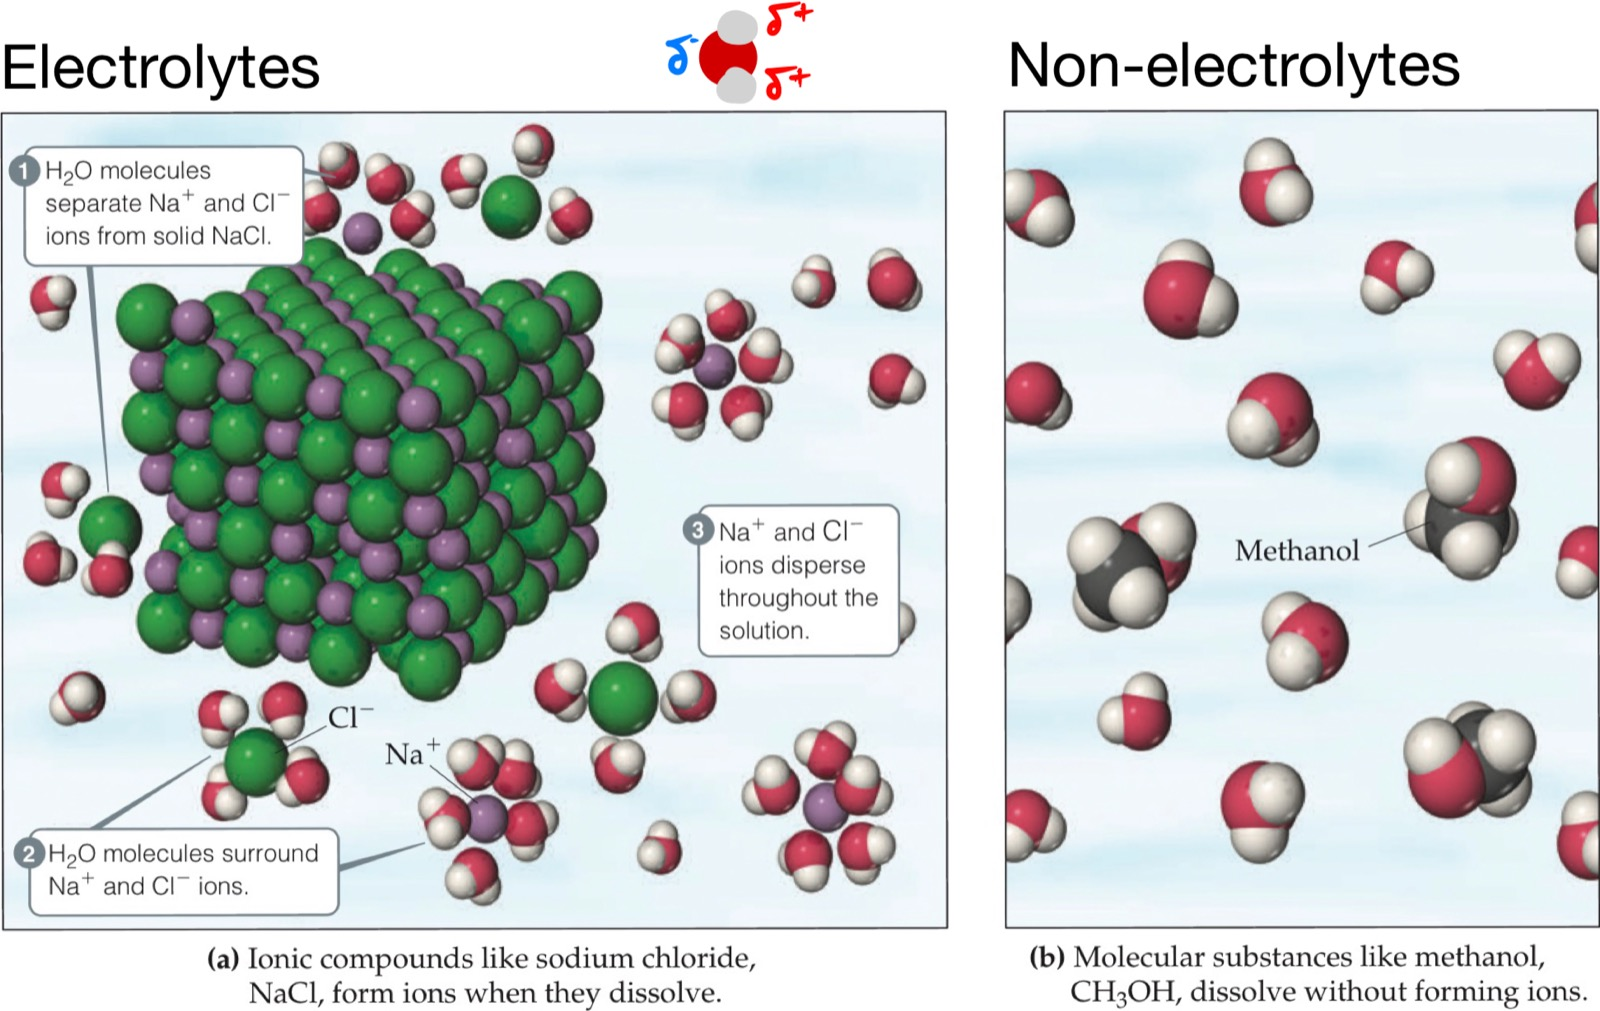
\includegraphics[width = 0.9\linewidth]{images/electrolytes_non_electrolytes.jpeg}
    \end{center}
\end{minipage}
\begin{minipage}{0.39\linewidth}
    \begin{center}
    \textbf{Neutralization Reaction}
        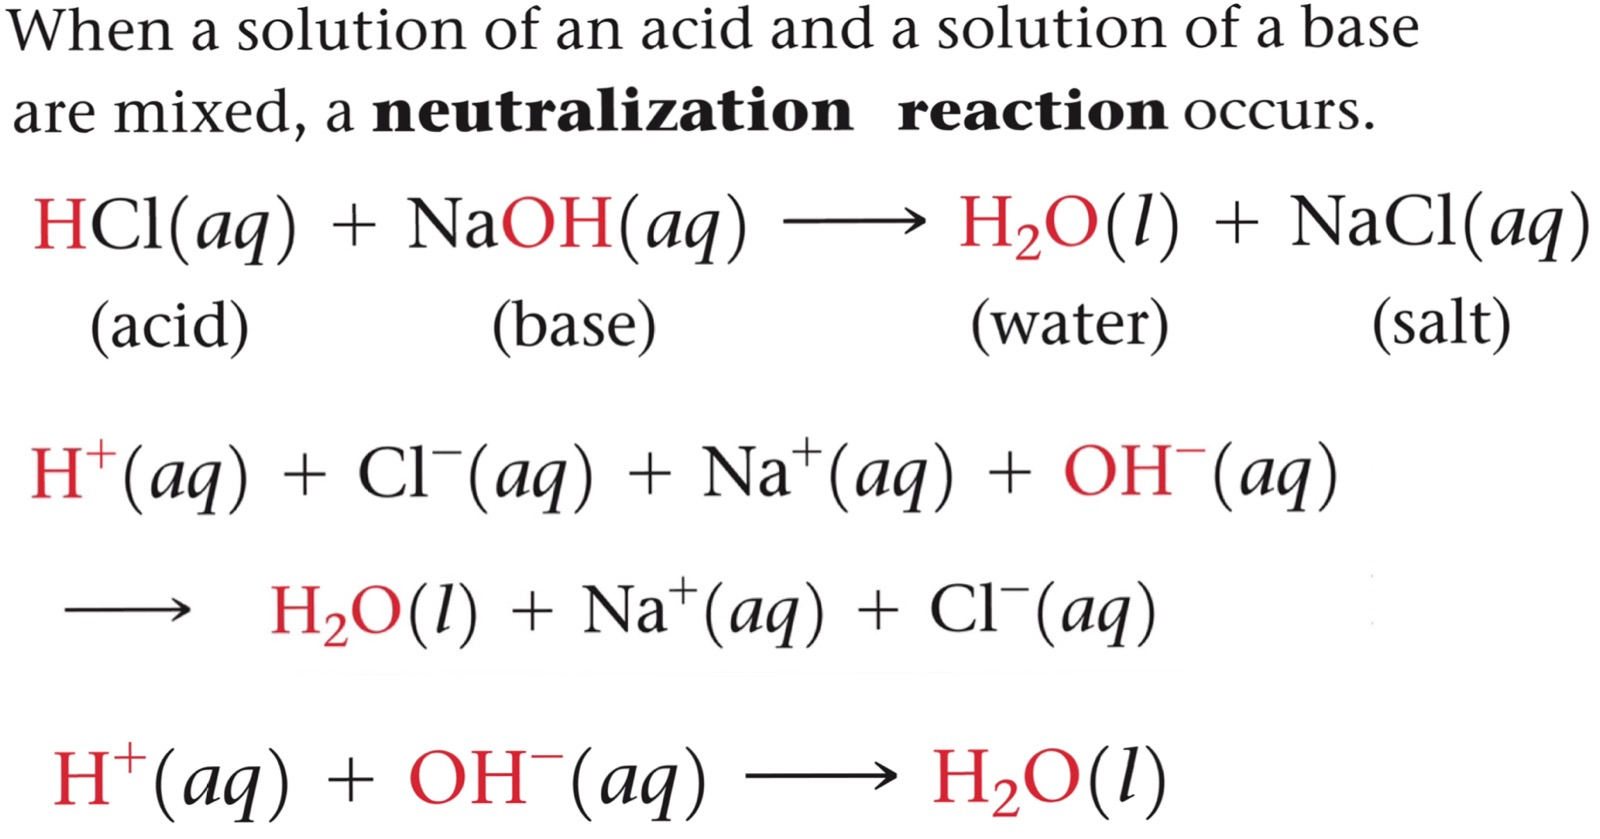
\includegraphics[width = \linewidth]{images/neutralization_reaction.jpeg}
    \end{center}
    \textbf{Concentration}\\
    \fbox{Molarity $= \frac{\text{moles solute}}{\text{volume of solution in L}}$}
\end{minipage}
\textbf{Thermodynamics of Solutions}\\
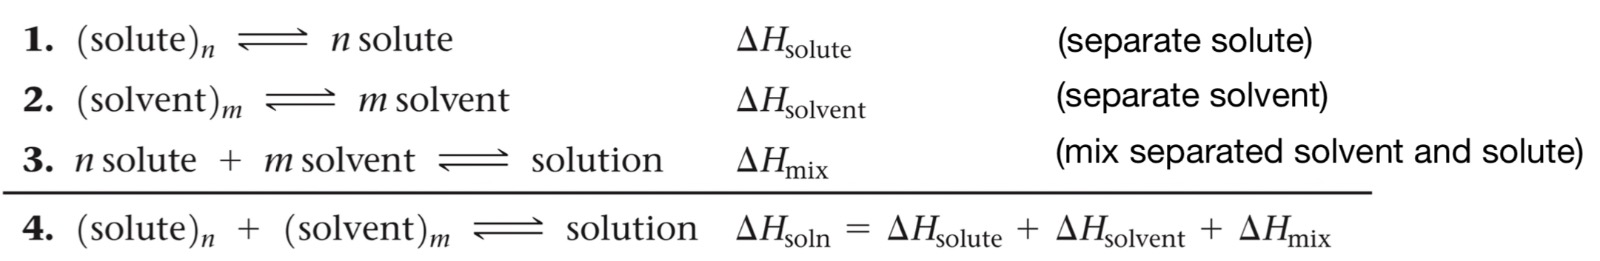
\includegraphics[width = 0.8\linewidth]{images/solvent_solution.jpeg}
\begin{center}
   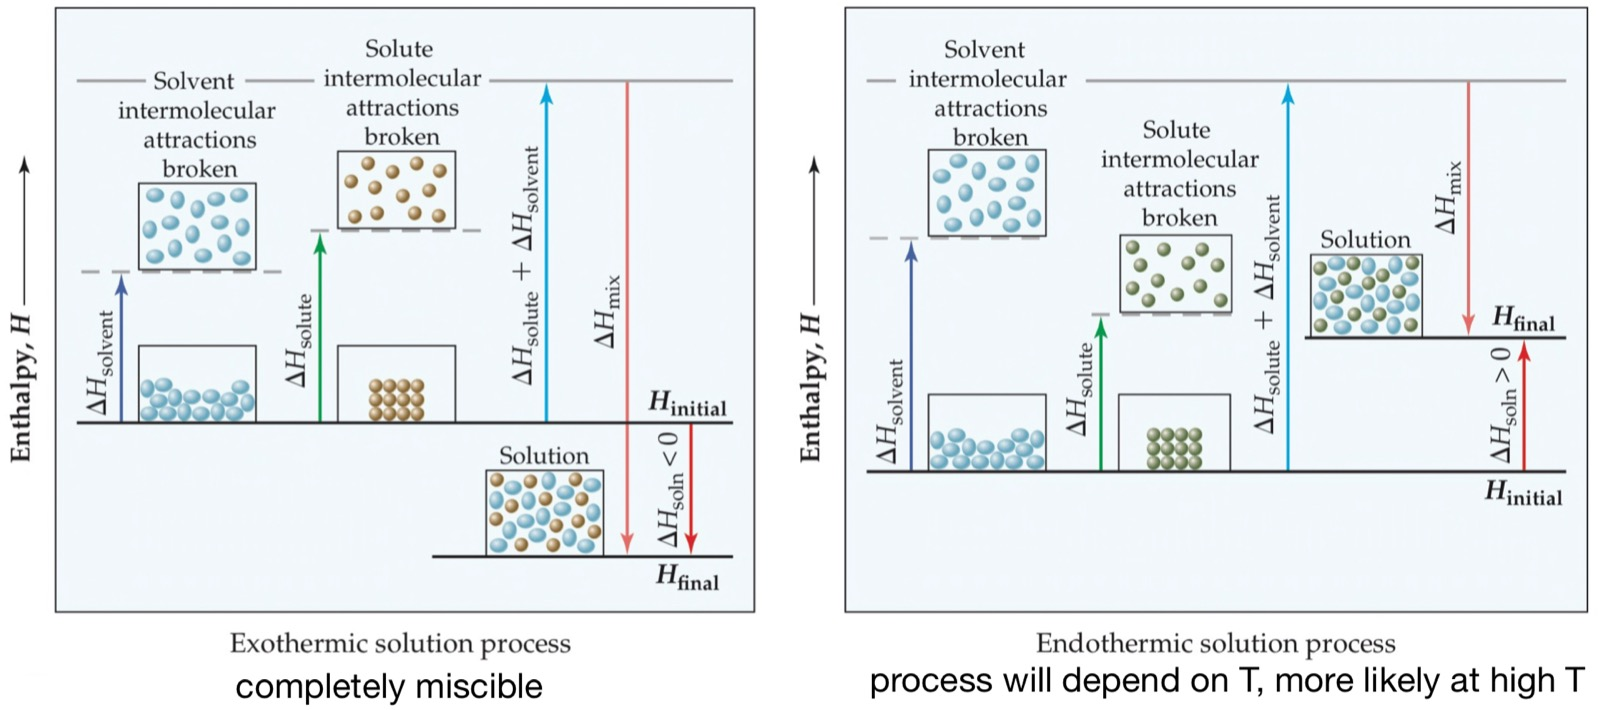
\includegraphics[width = 0.9\linewidth]{images/miscible_not_miscible.jpeg} 
   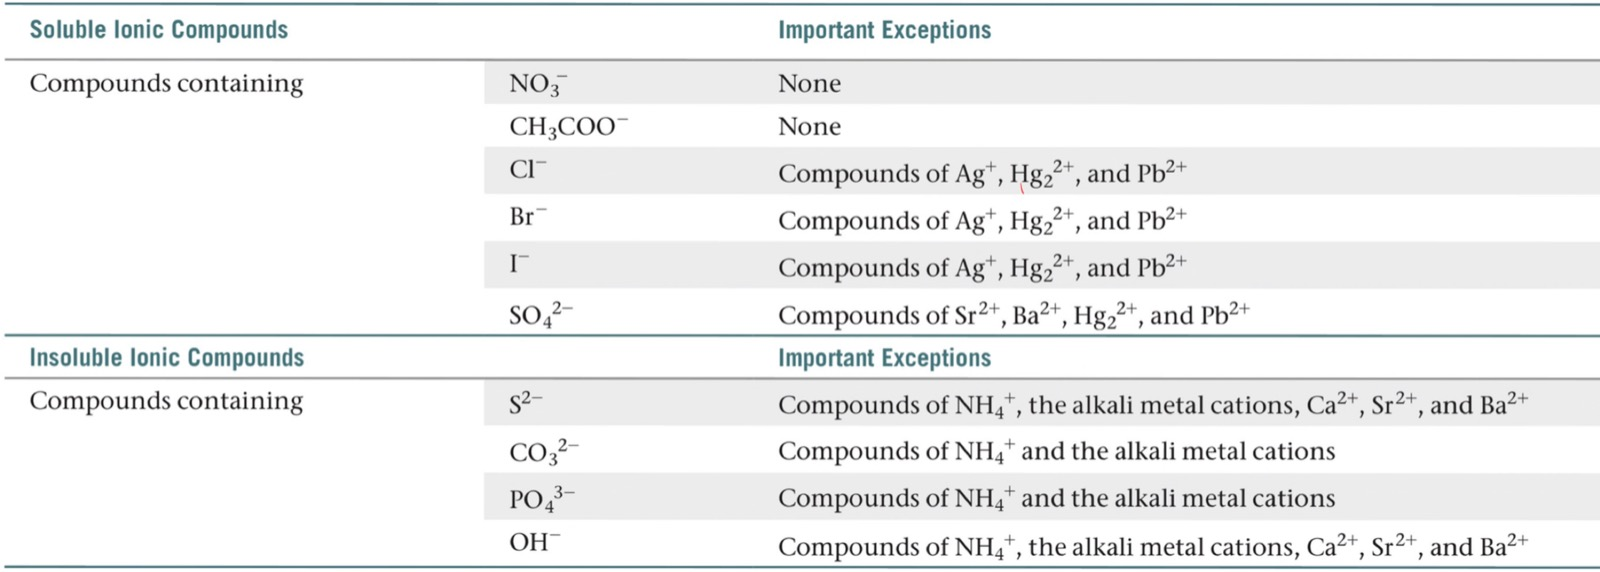
\includegraphics[width = 0.95\linewidth]{images/soluibility.jpeg}
\end{center}
\begin{minipage}{0.2\linewidth}
    \textbf{Gas Solubility}\\
    \fbox{$S_g = kP_g$}
\end{minipage}
\begin{minipage}{0.79\linewidth}
    \textbf{k}: Henry's law constant $[k] = \frac{mol}{m^3\cdot Pa}$, dependent on solute and solvent\\
    \textbf{$P_g$}: Gas partial pressure above liquid $[P_g] = Pa$
\end{minipage}
\textbf{Colligative Properties}\\
Changes only depend on the amount of solute added and not the type of solute\\
\begin{minipage}{0.35\linewidth}
    \textbf{1. Boiling-Point Elevation}\\
    \fbox{$\Delta T_b = T_b$(solution)$- T_b$(solvent) $= i K_b m$}\\
    $m \equiv$ molalilty of solute\\
    $k_b \equiv$ molal bp. elevation constant\\
    $i \equiv$ van't Hoff factor ($NaCl \longrightarrow i = 2$)
\end{minipage}
\begin{minipage}{0.32\linewidth}
    \textbf{2. Vapor-Pressure Lowering \\(Raoult's Law)}\\
    \fbox{$P_{vap}^{sol} = X_{solvent} \cdot P_{vap}^{pure}$}\\
    $P_{vap}^{sol} \equiv$ vapour pressure of solution\\
    $X_{solvent} \equiv$ mole fraction solvent\\
    $P_{vap}^{pure} \equiv$ vapour pressure of pure solvent 
\end{minipage}
\begin{minipage}{0.32\linewidth}
    \textbf{3. Freezing-Point Depression}\\
    \fbox{$\Delta T_f = T_f$(solution)$- T_f$(solvent) $= -i K_f m$}\\
    $m \equiv$ molalilty of solute\\
    $k_f \equiv$ molal fp. depression constant\\
    $i \equiv$ van't Hoff factor
\end{minipage}


    \subsection{Osmotic Pressure}{
The pressure required to counteract osmotic flow of a liquid is called the osmotic pressure. The osmotic flow tries to equalize concentrations across semi-permeable membranes.\\
\begin{minipage}{0.3\linewidth}
    \fbox{$\Pi = i (\frac{n}{V}) RT = iMRT$}\\
\end{minipage}
\begin{minipage}{0.69\linewidth}
    $\Pi \equiv$ osmotic pressure\\
    $\frac{n}{V} = M \equiv$ molarity\\
    $i \equiv$ van't Hoff factor
\end{minipage}}



% --------------------------------------
%5.5 Ideal Gases
%---------------------------------------
\subsection{Ideal Gases}
\begin{minipage}{0.33\linewidth}
    Assumptions for ideal gases:\\
    $\circ$ Gas particles do not interact\\
    $\circ$ Gas particles have no volume\\
    \textbf{$1^{st}$ Gas (Boyle's) Law}\\
    \fbox{$P \cdot V = const.$ if $n$ \& $T const.$}\\
    \textbf{$2^{nd}$ Gas (Charles') Law}\\
    \fbox{$\frac{V}{T} = const.$ if $n$ \& $P const.$}\\
    \textbf{$3^{rd}$ Gas (Avogadro's) Law}\\
    \fbox{$\frac{V}{n} = const.$ if $P$ \& $T const.$}\\
    \textbf{Van der Waals Equations}\\
    \fbox{$(P + \frac{n^2 a}{V^2})(V - nb) = nRT$}\\
    a, b are correction factors\\
    $\frac{n^2a}{V^2}$ corrects interactions at low $T$.\\
    $nb$ corrects non-neglible volume occupied by molecules at high $P$
\end{minipage}
\begin{minipage}{0.33\linewidth}
    \textbf{Ideal Gas Law}\\
    \fbox{$P\cdot V = n\cdot R \cdot T$}\\
    \textbf{Molar Gas Volume (STP)}\\
    \fbox{$V_{mol} = 22.41 l = 22.41 dm^3$}\\
    \textbf{Atmospheric Pressure}\\
    \fbox{\begin{varwidth}{\textwidth}
    \centering
    $P_{atm} = 760 mmHg = 760 Torr$\\ $ = 1 atm = 101325 Pa = 1.01325 bar$
    \end{varwidth}}
    \textbf{Barometer}\\
    \fbox{$P = \rho g h$}
    \begin{center}
        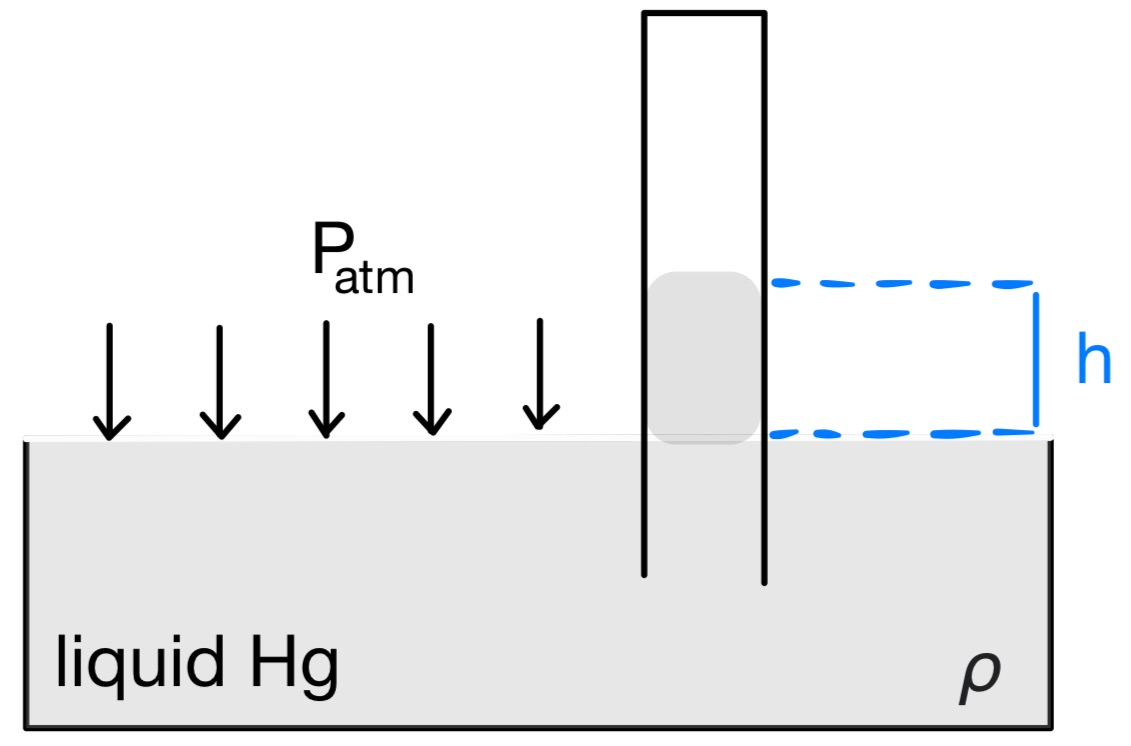
\includegraphics[width = 0.9\linewidth]{images/Barometer.jpeg}
    \end{center}
\end{minipage}
\begin{minipage}{0.33\linewidth}
    \textbf{Density (IGL)}\\
    \fbox{$\rho = \frac{P}{R\cdot T} \cdot M_w$}\\
    \textbf{Molecular Weight (IGL)}\\
    \fbox{$M_w = \frac{\rho R T}{P}$}\\
    \textbf{Partial Pressures \\ Dalton's Law}\\
    \fbox{\begin{varwidth}{\textwidth}
    \centering
    $P_{tot} = \sum_i P_i$\\ $P_i = \frac{n_i}{n_{tot}} \cdot P_{tot} = \chi_i \cdot P_{tot}$
    \end{varwidth}}\\
    \textbf{Manometer}\\
    \fbox{$P_{gas} = P_{atm} + \rho g h$}\\
    \begin{center}
        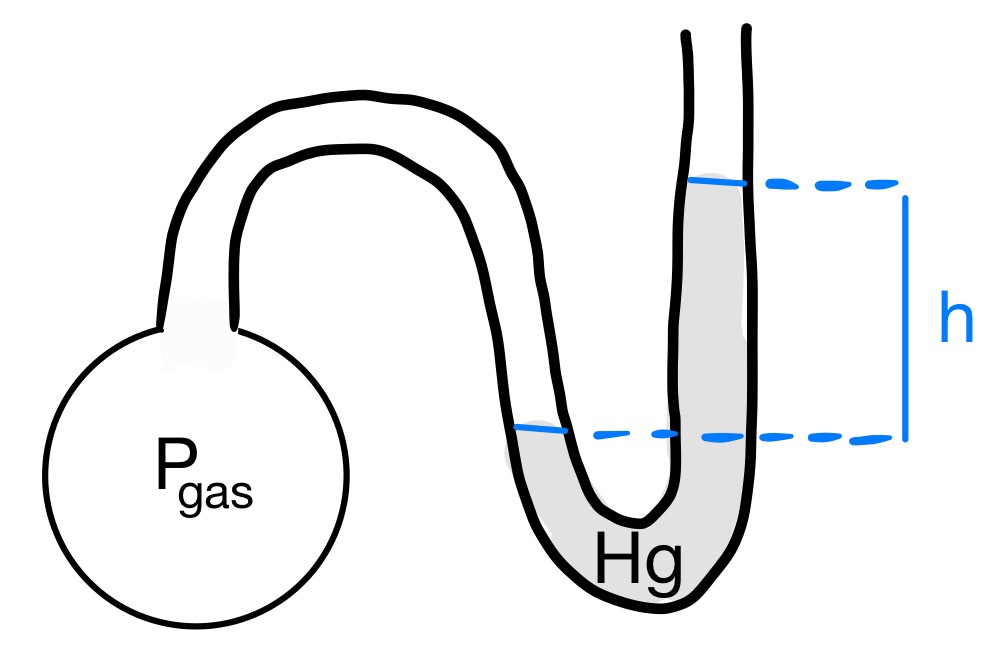
\includegraphics[width = 0.8\linewidth]{images/Manometer.jpeg}
    \end{center}
\end{minipage}
\begin{center}
    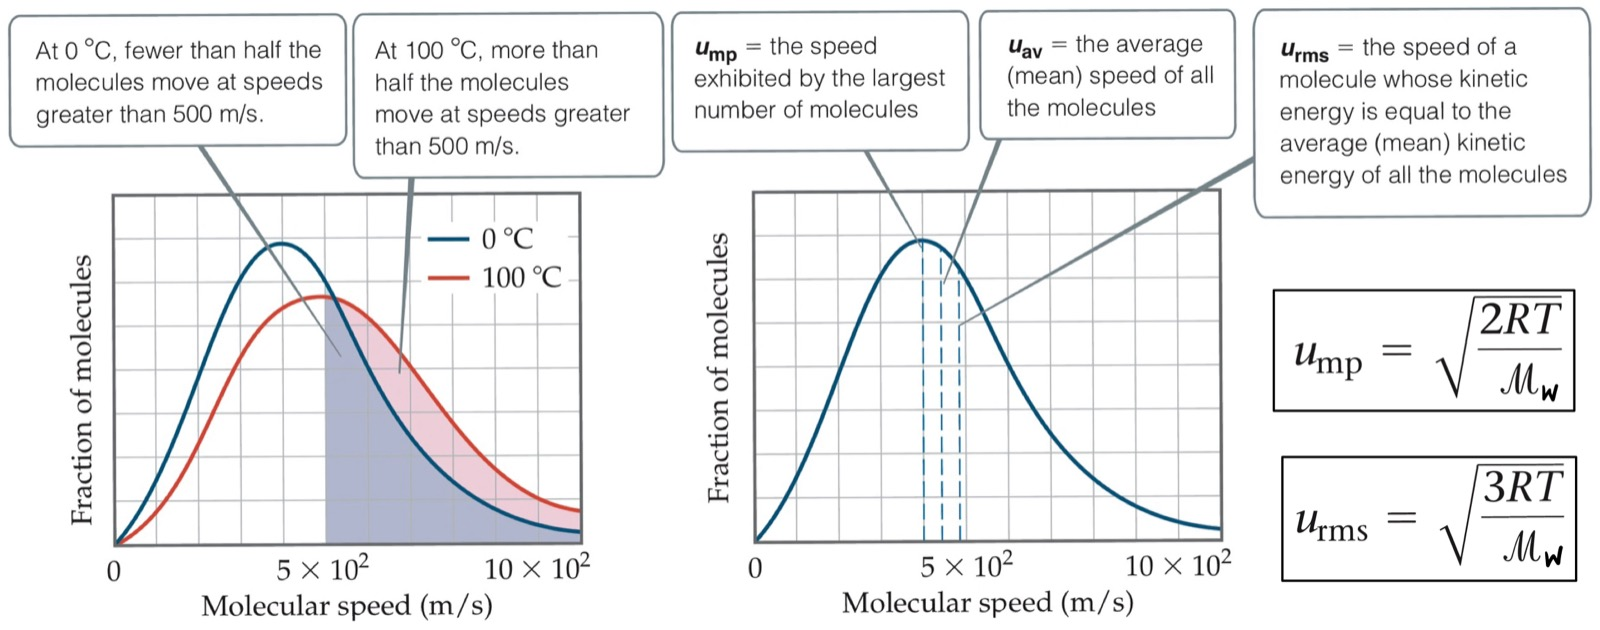
\includegraphics[width = 0.9\linewidth]{images/gas_kinetics.jpeg}
\end{center}

%---------------------------------------
%6. Thermodynamics
%---------------------------------------
\section{Thermodynamics}
%---------------------------------------
%6.1 The Three Laws of Thermodynamics
%---------------------------------------
\subsection{The Three Laws of Thermodynamics}
\textbf{\textcolor{red}{$1^{st}$ Law}}\\
\fbox{Energy can be converted from one form to another, but it is neither created nor destroyed.}\\
\textbf{\textcolor{red}{$2^{nd}$ Law}}\\
\fbox{\begin{varwidth}{\textwidth}
\centering
The entropy of the universe increases for any spontaneous process.\\ Reversible Process: $\Delta S_{univ} = \Delta S_{sys} + \Delta S_{surr} = 0$\\
Irreversible Process: $\Delta S_{univ} = \Delta S_{sys} + \Delta S_{surr} > 0$
\end{varwidth}}\\
\textbf{\textcolor{red}{$3^{rd}$ Law}}\\
\fbox{\begin{varwidth}{\textwidth}
The entropy of a pure, perfect crystalline substance at absolute zero is zero: $S (0K) = 0$. 
\\There is only one possible microstate.\\
$S = k ln(W) = k ln(1) = 0$
\end{varwidth}}\\
%---------------------------------------
%6.2 System and Internal Energy 
%---------------------------------------
\subsection{System and Internal Energy}
\begin{minipage}{0.75\linewidth}
\textbf{System Types and Internal Energy}\\
\fbox{\begin{varwidth}{\textwidth}
\textbf{Open}: Matter and energy can be exchanged with surroundings\\
\textbf{Closed:} Energy can be exchanged with surroundings (but not matter)\\
\textbf{Isolated:} Neither matter nor energy is exchanged with surroundings\\
$\Delta E = E_{final} - E_{initial}, \Delta E > 0 \longrightarrow$ system has gained $E$, $\Delta E < 0 \longrightarrow$ system has lost $E$.
\end{varwidth}}\\    
\end{minipage}
\begin{minipage}{0.24\linewidth}
\textbf{State functions}\\
$\circ$ Gibbs free energy, enthalpy, entropy and internal energy are state functions\\
$\circ$ Work is not a state function
\end{minipage}
\begin{minipage}{0.65\linewidth}
\textbf{Internal Energy}\\
\fbox{\begin{varwidth}{\textwidth}
$\Delta E = q + w$, $q \equiv$ heat is added to system, $w \equiv$ work done on system\\
$q > 0$ heat is added to system (\textcolor{blue}{endothermic}) \hspace{3pt} $w > 0$ work done on system\\
$q < 0$ heat is lost by system (\textcolor{blue}{exothermic}) \hspace{8pt} $w < 0$ work done by system
\end{varwidth}}\\  
\textbf{Calorimetry} \hspace {8pt} \textbf{e.g.} $H_{2}O$: $c_s = 4.18 \frac{J}{g \cdot K}$\\
\fbox{\begin{varwidth}{\textwidth}Heat capacity $=$ heat required for $\Delta T = 1K$ for specific substance\\
$q = n \cdot c_m \cdot \Delta T$ \hspace{3pt} $c_m \equiv$ molar heat capacity \hspace{3pt} $[c_m] = \frac{J}{mol \cdot K}$\\
$q = n \cdot c_s \cdot \Delta T$ \hspace{3pt} $c_s \equiv$ specific heat capacity \hspace{3pt} $[c_s] = \frac{J}{g \cdot K}$
\end{varwidth}}   
\end{minipage}
\begin{minipage}{0.27\linewidth}
\begin{center}
    \textbf{Exothermic Reaction}
    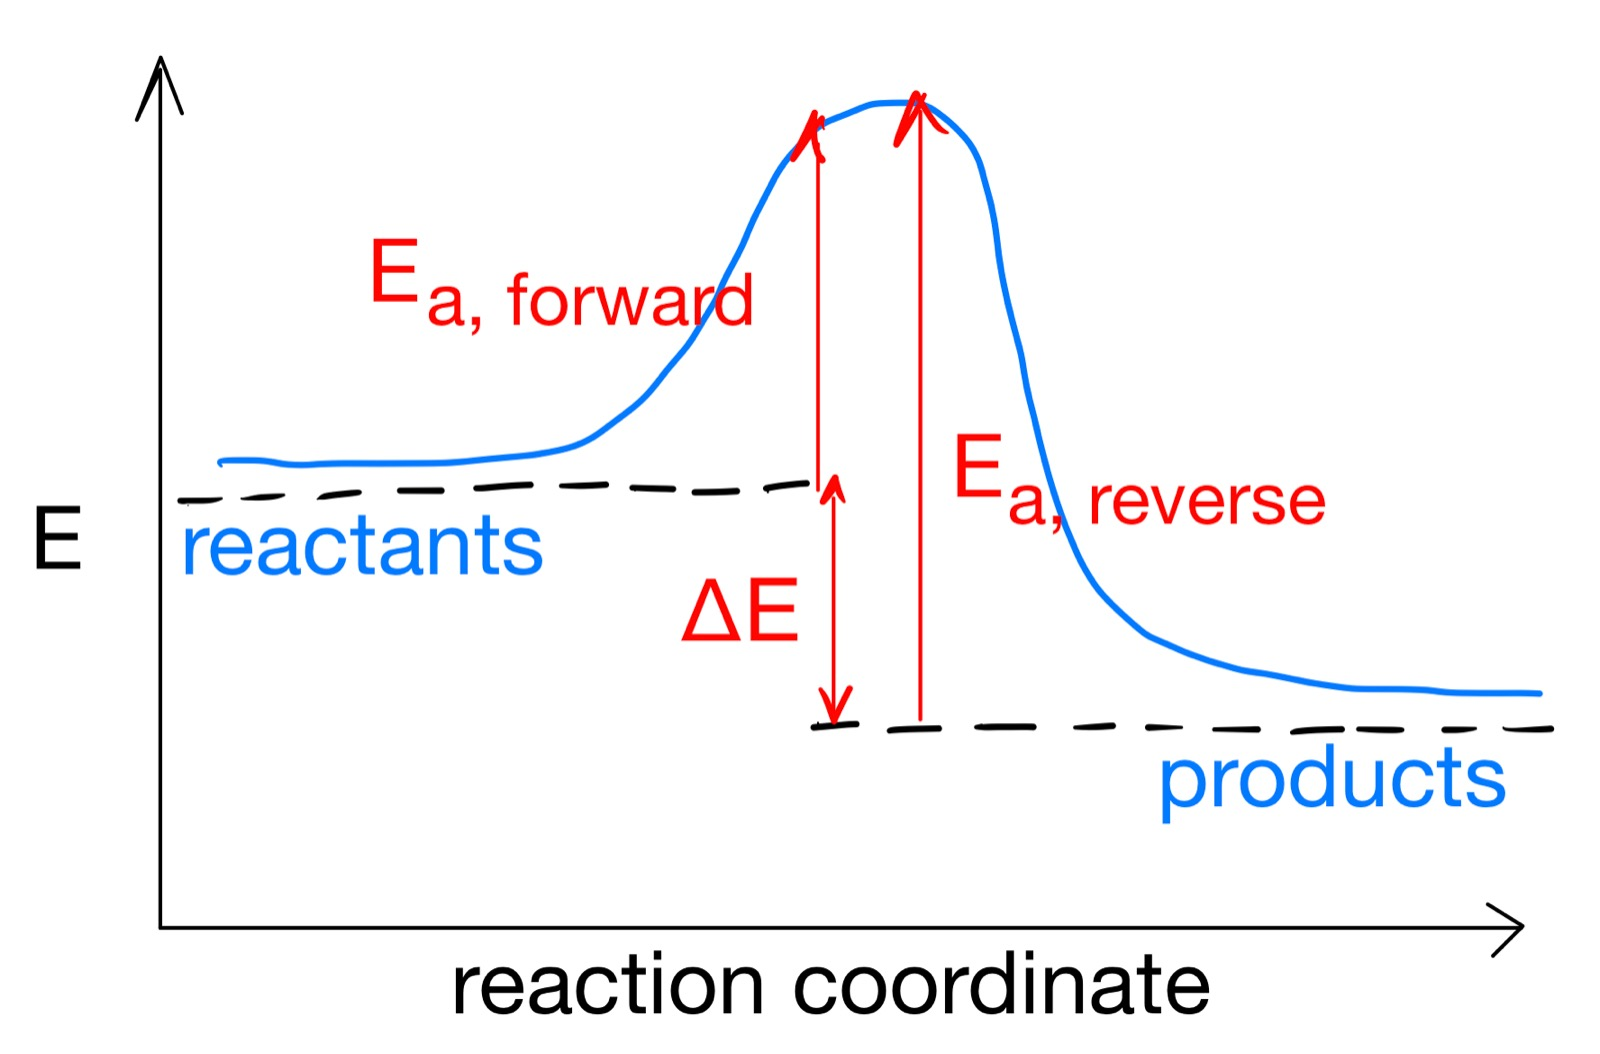
\includegraphics[width = \linewidth]{images/exothermic reaction.jpeg}
\end{center}
\begin{center}
    \textbf{Endothermic Reaction}
    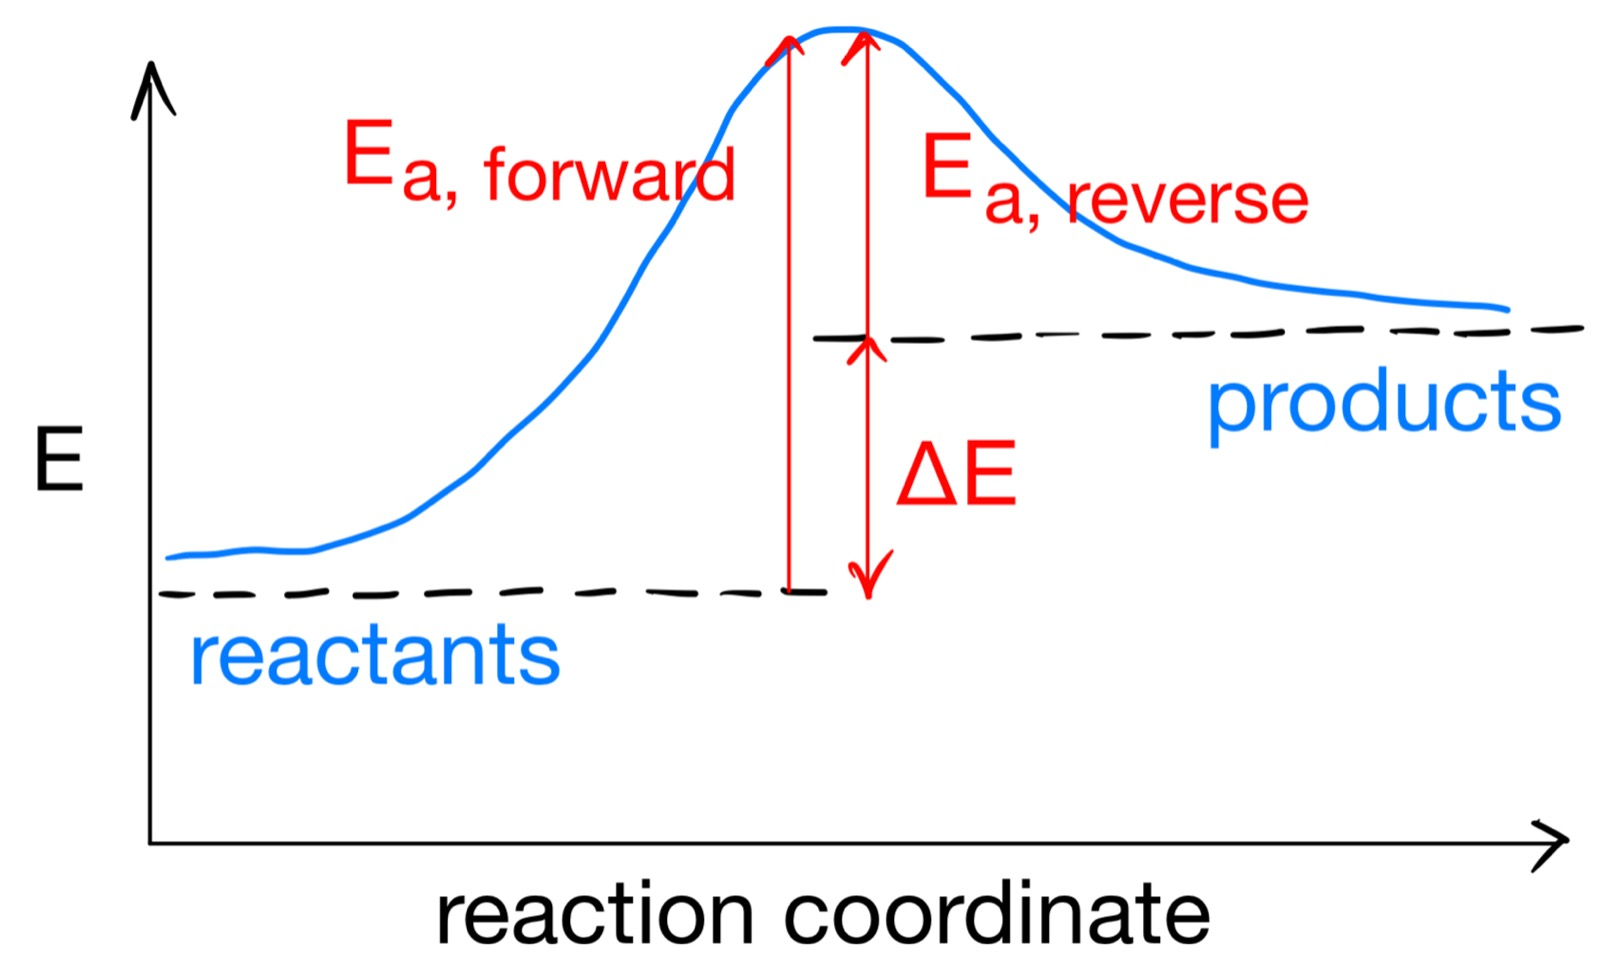
\includegraphics[width = \linewidth]{images/endothermic reaction.jpeg}
\end{center}   
\end{minipage}
%---------------------------------------
%6.3 Enthalpy
%---------------------------------------
\subsection{Enthalpy}
\begin{minipage}{0.49\linewidth}
\textbf{Enthalpy}\\
\fbox{\begin{varwidth}{\textwidth}
$H \equiv E + PV = $ internal energy $+$ pressure-volume work\\
$\Delta H = \Delta E + P \Delta V = (q_p + w) - w ) = q_b$\\
Change in enthalpy is equal to heat at constant $P$\\
$\longrightarrow$ if $\Delta V$ small $\Delta H \simeq \Delta E$ \hspace{5pt} $w = -P\cdot V$
\end{varwidth}}\\
\textbf{Enthalpies of Reaction (Heat of Reaction}\\
\fbox{\begin{varwidth}{\textwidth}$\Delta H = H_{final} - H_{initial}$ \hspace{5pt} $\Delta H_{forward} = - \Delta H_{reverse}$\\
$\Delta H = H_{products} - H_{reactants}$\\
$\Delta H_{rxn}^{\circ} = \sum n \Delta H_f^{\circ}$ (products) $- \sum m \Delta H_f^{\circ}$ (reactants)
\end{varwidth}}
\end{minipage}
\begin{minipage}{0.50\linewidth}
\begin{center}
\fbox{ 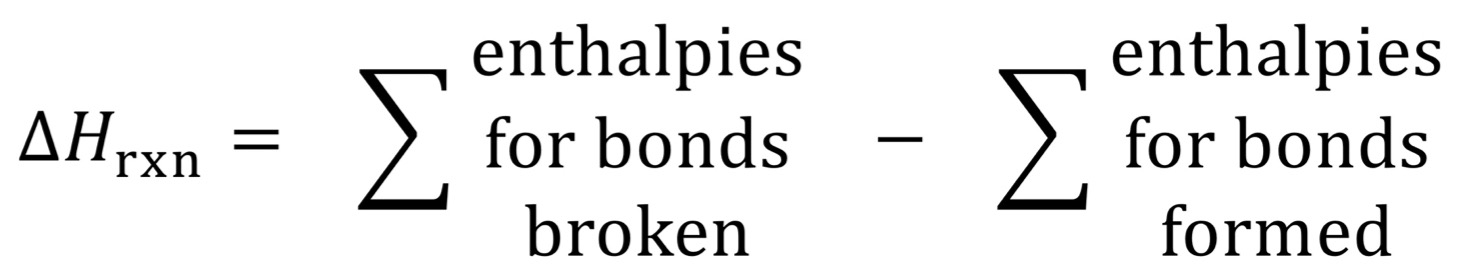
\includegraphics[width = 0.65\linewidth]{images/enthalpy.jpeg}}
\end{center}
\begin{center}
    \textbf{Pressure-Volume Work}\\
    \fbox{$W = -P (V_{final} - V_{initial})$}\\
\end{center}
\textbf{\textcolor{red}{Hess's Law}}\\
\fbox{\begin{varwidth}{\textwidth} If a reaction can be written in steps, then enthalpy \\
change of reaction is sum of enthalpy changes for steps.\\
$\Delta H_{rxn} = \Delta H_1 + \Delta H_2 + \Delta H_3 + ...$
\end{varwidth}}
    
\end{minipage}
\umbruch
%---------------------------------------
%6.4 Entropy
%---------------------------------------
\subsection{Entropy}
\textbf{Entropy S}\\
\fbox{\begin{varwidth}{\textwidth}
A measure of the tendency for E to spread, which reduces system's ability to do work\\ (related to randomness or disorder in system).\\
$\Delta S = \frac{q_{rev}}{T}$ \hspace{3pt} $q_{rev} \equiv$ heat flow for reversible process \hspace{3pt} $T \equiv$ absolute temperature\\
$\Delta S$ for phase changes (melting/boiling) \hspace{5pt} isothermal $\longrightarrow$ $q_{rev} = \Delta H_{fus}$ \& $q_{rev} = \Delta H_{vap}$
\end{varwidth}}\\
\begin{minipage}{0.58\linewidth}
\textbf{Boltzmann Equation}\\
\fbox{\begin{varwidth}{\textwidth}
    $S = k_B ln(W)$ \hspace{5pt} $W = \# $ microstates \hspace{3pt} $k_B = 1.38 \cdot 10^{-23} \frac{J}{K}$\\
    $\Delta S = k_B ln(W_{final}) - k_B ln(W_{initial}) = k_B ln(\frac{W_final}{W_initial})$\\
    Entropy increases with the number of microstates of the system. 
    
\end{varwidth}}

\end{minipage}
\begin{minipage}{0.40 \linewidth}
\textbf{$\Delta$S for Chemical Reactions}\\
\fbox{\begin{varwidth}{\textwidth}
$\Delta S^{\circ} = \sum n S^{\circ}$ (products) $- \sum m S^{\circ}$ (reactants\\
$\Delta S^{\circ} = \Delta S_{sys}^{\circ} \equiv$ standard molar entropies
\end{varwidth}}\\
\textbf{$\Delta S_{surr}$}\\
\fbox{$\Delta S_{surr} = \frac{q_{surr}}{T} = \frac{-q_{sys}}{T} = \frac{-\Delta H_{rxn}^{\circ}}{T}$ [at constant P]}
\end{minipage}
%---------------------------------------
%6.5 Gibbs Free Energy
%---------------------------------------
\subsection{Gibbs Free Energy}
\begin{minipage}{0.71\linewidth}
\textbf{Gibbs Free Energy}\\
\fbox{\begin{varwidth}{\textwidth}
$G = H - TS$ \hspace{5pt} $\Delta G^{\circ} = \Delta H^{\circ} - T \Delta S^{\circ}$\\
$\circ$ If $\Delta G < 0$, the reaction is spontaneous in the forward direction. (\textcolor{blue}{irreversible})\\
$\circ$ If $\Delta G = 0$, the reaction is at equilibrium. (\textcolor{blue}{reversible})\\
$\circ$ If $\Delta G > 0$, the reaction is nonspontaneous in the forward direction (work must be\\
done to make it occur) but the reverse reaction is spontaneous.
\end{varwidth}}\\
\textbf{Standard Free Energy of Formation}\\
\fbox{$ \Delta G ^{\circ} = \sum n \Delta G_f^{\circ}$ (products) $- \sum m \Delta G_f^{\circ}$ (reactants)}

\end{minipage}
\begin{minipage}{0.26\linewidth}
\textbf{Pure Substances}\\
\fbox{\begin{varwidth}{\textwidth}Gibbs Free energy and enthalpy of pure substances are 0
\end{varwidth}}
\end{minipage}\\
\textbf{The Importance of $T$}\\
\begin{tabular}{c|c|c|c|c|c}
    Example & $\Delta H$ & $\Delta S$ & $-T \Delta S$ & $\Delta G$ & Temperature dependence \\ \hline
    $2 O_3 (g) \longrightarrow 3 O_2 (g)$ & \colorbox{red}{$-$} & \colorbox{green}{$+$}  & \colorbox{red}{$-$} & \colorbox{red}{$-$} & spontaneous at all $T$\\
    $3 O_2 (g) \longrightarrow 2 O_3 (g)$ & \colorbox{green}{$+$} & \colorbox{red}{$-$} & \colorbox{green}{$+$} & \colorbox{green}{$+$}& nonspontaneous at all $T$\\
    $H_2 O (l) \longrightarrow H_2O (s)$ & \colorbox{red}{$-$} & \colorbox{red}{$-$} &\colorbox{green}{$+$}& \colorbox{yellow}{$+$ or $-$}& spontaneous at low $T$\\
    $H_2O(s) \longrightarrow H_2O(l)$ &\colorbox{green}{$+$} &\colorbox{green}{$+$} & \colorbox{red}{$-$} 
    & \colorbox{yellow}{$+$ or $-$}& spontaneous at high $T$
\end{tabular}\\
\textbf{Spontaneous vs. Nonspontaneous Processes}\\
\fbox{\begin{varwidth}{\textwidth}
$\circ$ If process is spontaneous on one direction $\longrightarrow$ nonspontaneous in reverse\\
$\circ$ Nonspontaneous does not mean impossible (add energy)\\
$\circ$ Experimental conditions matter\\
$\circ$ All spontaneous processes are irreversible (requires work to return to initial state).
\end{varwidth}}\\
\textbf{Reversible vs. Irreversible Processes}\\
\fbox{\begin{varwidth}{\textwidth}\textcolor{blue}{Reversible}: Process can be reversed with no change to surroundings. \hspace{3pt}
$\Delta S_{univ} = 0$\\
\textcolor{blue}{Irreversible}: Surroundings change when process is reversed (e.g. heat transfer) \end{varwidth}}

%---------------------------------------
%7. Kinetics
%---------------------------------------
\section{Kinetics}
%---------------------------------------
%7.1 Reactions Rates
%---------------------------------------
\subsection{Reaction Rates}
\begin{minipage}{0.5 \linewidth}
$\circ$ Convention: Reaction rates are always positive\\
\fbox{\begin{varwidth}{\textwidth}$Rate = -\frac{1}{\alpha}\frac{d[A]}{dt} = -\frac{1}{\beta}\frac{d[B]}{dt} = \frac{1}{\gamma}\frac{d[C]}{dt} = \frac{1}{\delta}\frac{d[D]}{dt}$
\end{varwidth}}\\
\begin{minipage}{0.49\linewidth}
\textbf{Reaction Order}\\
\fbox{$ Rate = k [A]^m [B]^n$}\\    
\end{minipage}
\begin{minipage}{0.5\linewidth}
$k:$ rate constant\\
$m, n$: rxn order\\
$m+n$: overall rxn order     
\end{minipage}
   
\end{minipage}
\begin{minipage}{0.49\linewidth}
   
    \begin{center}
     \textbf{Examples}\\
        \begin{tabular}{c|c}
         Overall rxn order & units of k  \\ \hline
         0 & $M s^{-1}$\\
         $\frac{1}{2}$ & $M^{1/2}s^{-1}$\\
         1 & $s^{-1}$\\
         2 & $M^{-1}s^{-1}$\\
         3 & $M^{-2}s^{-1}$
    \end{tabular}    
    \end{center}

\end{minipage}
%---------------------------------------
%7.2 Rate Laws
%---------------------------------------
\subsection{Rate Laws}
\begin{minipage}{0.33\linewidth}
    \begin{center}
        \textbf{Zero Order}\\
        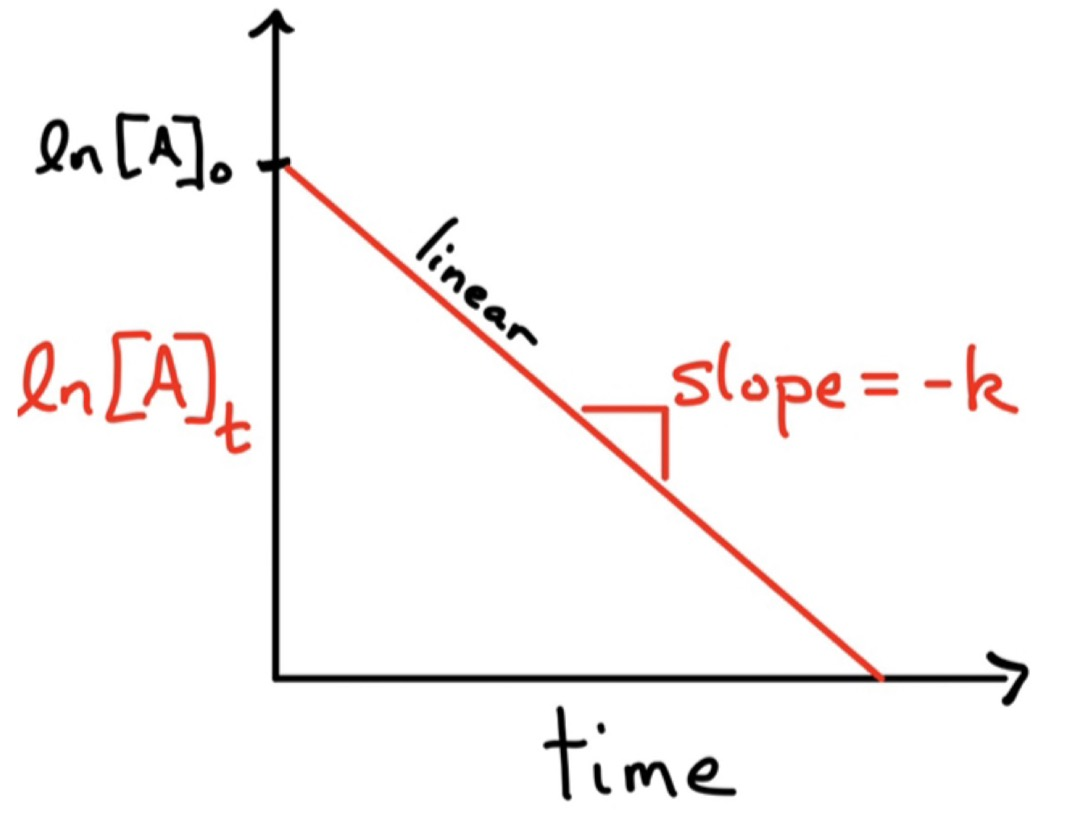
\includegraphics[width = \linewidth]{images/0 order.jpeg}\\
        \fbox{$[A]_t = - kt + [A]_0$}\\
        \fbox{$t_{1/2} = \frac{[A]_0}{2k}$}
    \end{center}
    
\end{minipage}
\begin{minipage}{0.33\linewidth}
    \begin{center}
        \textbf{First Order}\\
        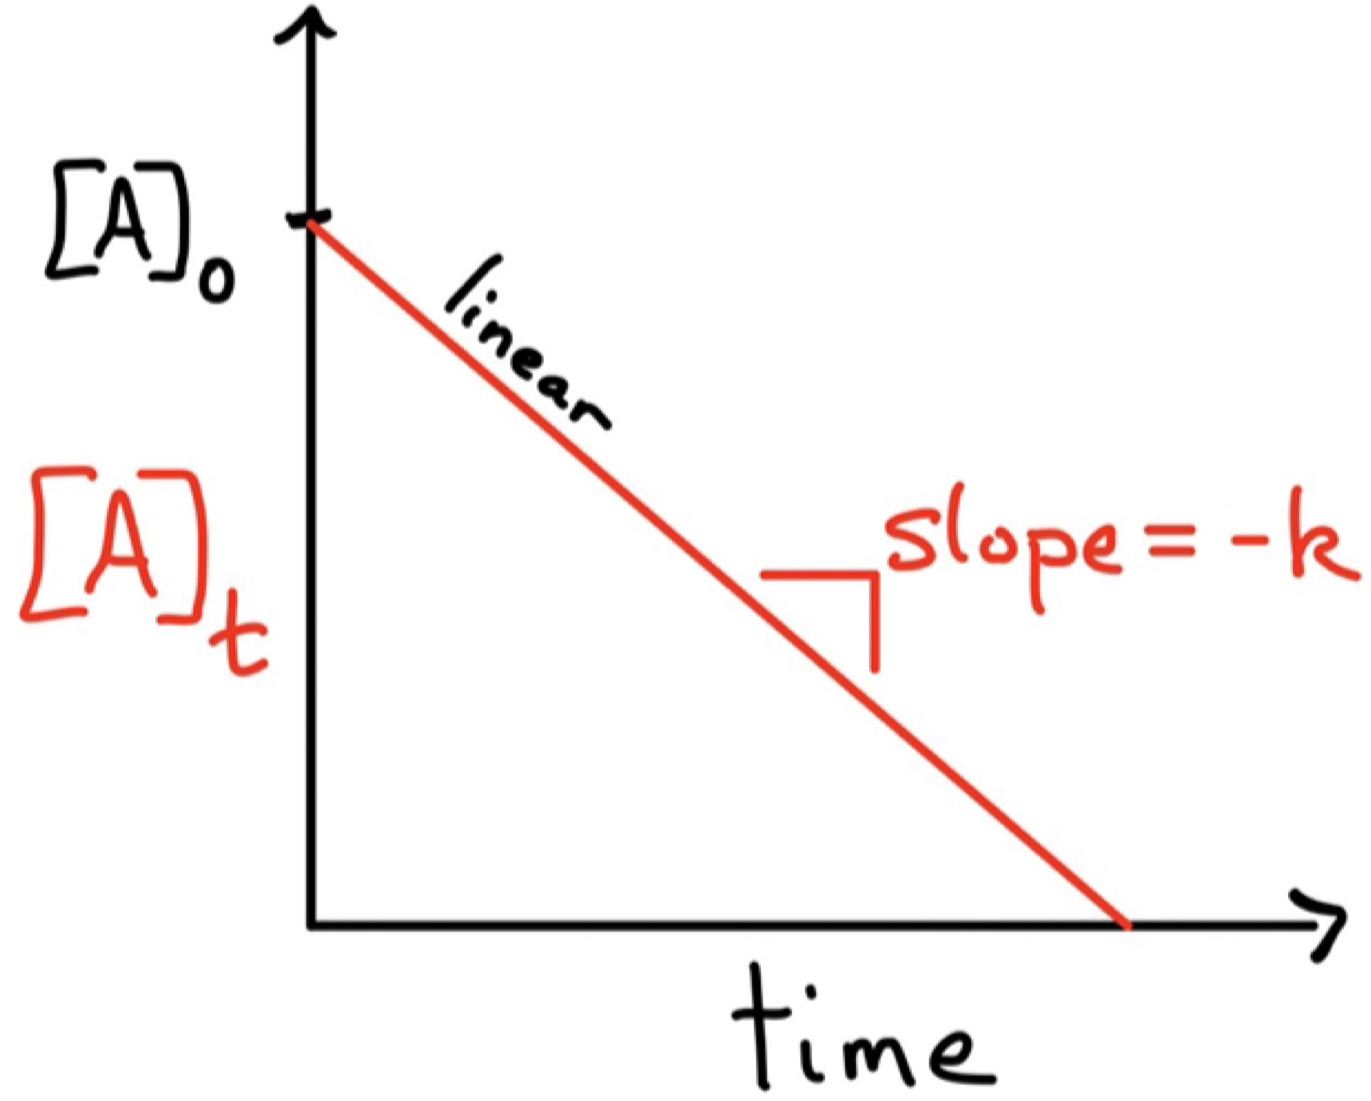
\includegraphics[width = \linewidth]{images/1st Order.jpeg}\\
        \fbox{$ln([A]_t) = - kt + ln([A]_0)$}\\
        \fbox{$t_{1/2} = \frac{0.693}{k}$}
    \end{center}
    
\end{minipage}
\begin{minipage}{0.33\linewidth}
    \begin{center}
        \textbf{Second Order}\\
        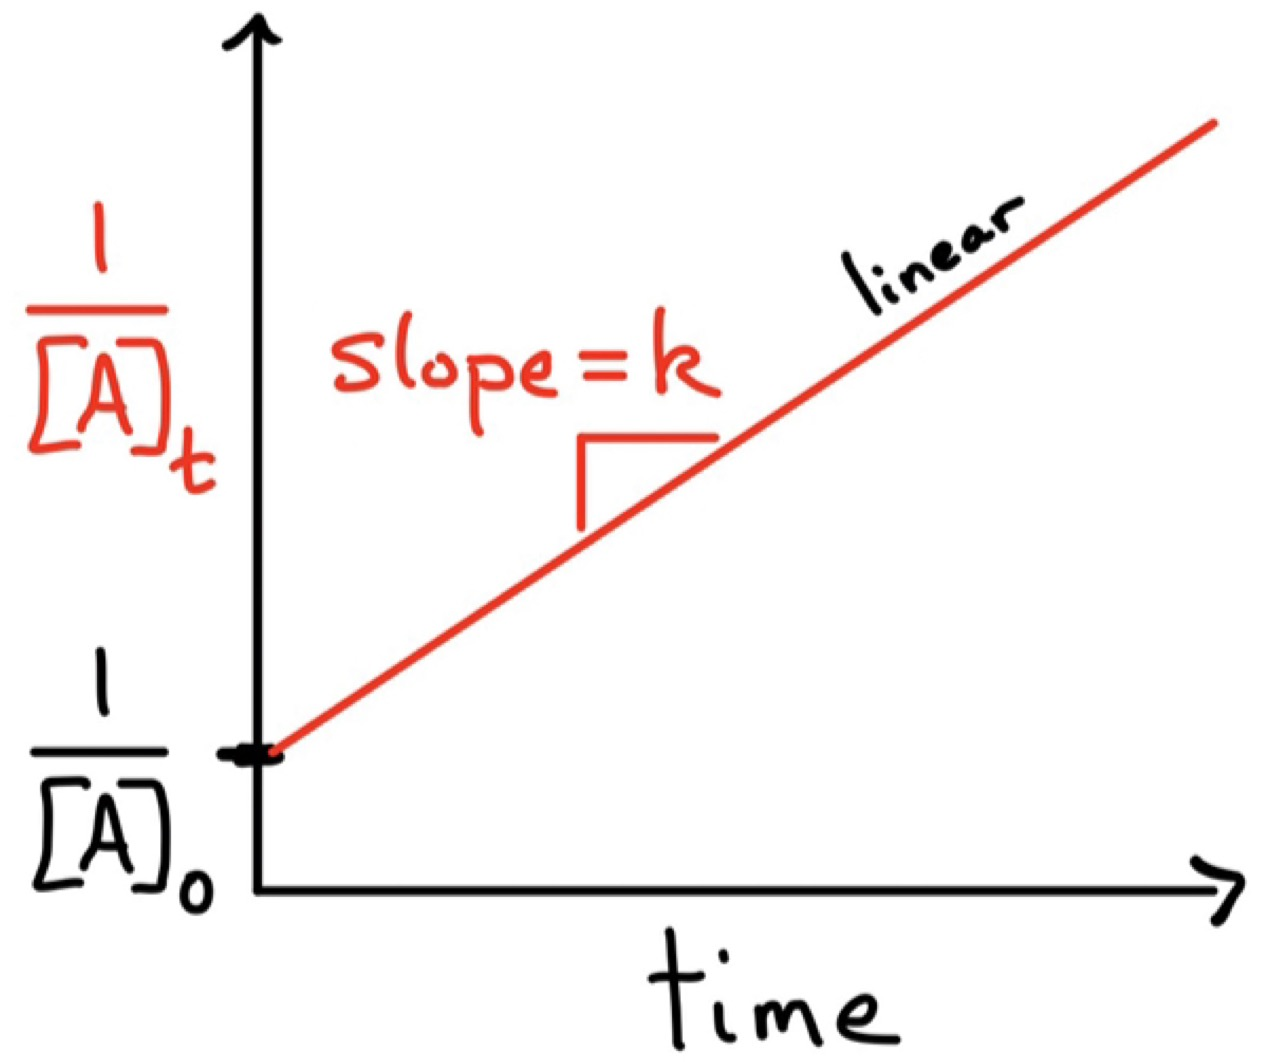
\includegraphics[width = \linewidth]{images/2nd order.jpeg}\\
        \fbox{$\frac{1}{[A]_t} = kt + \frac{1}{[A]_0} $}\\
        \fbox{$t_{1/2} = \frac{[A]_0}{2k}$}
    \end{center}
    
\end{minipage}
\begin{minipage}{0.3\linewidth}
    \begin{center}
        \fbox{$[A]_t = [A]_0 e^{-kt}$}
    \end{center}
\end{minipage}
\begin{minipage}{0.3\linewidth}
    \begin{center}
        $[A]_t \equiv$ Concentration of A at time t\\
        $[A]_0 \equiv$ Concentration of A at time $t = 0$
    \end{center}
\end{minipage}
%---------------------------------------
%7.3 Reaction Mechanisms
%---------------------------------------
\subsection{Reaction Mechanisms}
\begin{minipage}{0.65\linewidth}
\textbf{Arrhenius Equation}\\
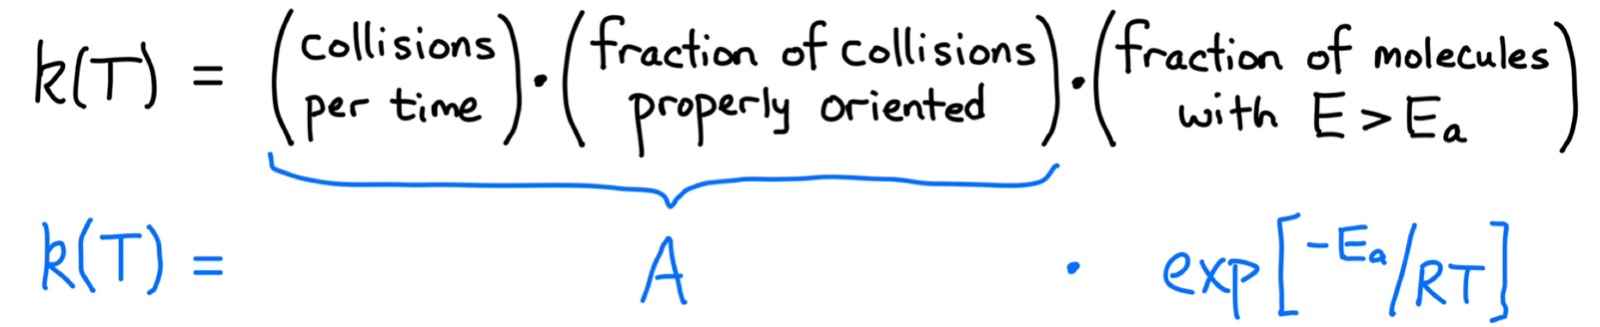
\includegraphics[width = 0.95\linewidth]{images/Arrhenius_Equation.jpeg}

\begin{minipage}{0.4\linewidth}
    \fbox{$k(T) = A \cdot exp[\frac{-E_a}{RT}]$}\\
    \fbox{$ln(\frac{k_1}{k_2}) = \frac{E_a}{R}(\frac{1}{T_2} - \frac{1}{T_1})$}
\end{minipage}
\begin{minipage}{0.35\linewidth}
    \begin{center}
        $E_a \equiv$ activation energy\\
        $R \equiv$ universal gas constant\\
        $T \equiv$ absolute Temperature $[T] = K$
    \end{center}
\end{minipage}
$\circ$ Approximation: Increasing temperature by $10 ^{\circ}C$ doubles the rate of reaction.\\
\textbf{Reaction Mechanism/ Molecularity}\\
\begin{tabular}{c|c|c}
     Molecules colliding& Molecularity & Example  \\ \hline
     one & Unimolecular & $A \longrightarrow Products$\\
     two & Bimolecular & $A + A \longrightarrow Products$\\
     three & Termolecular & $A + A + A \longrightarrow Products$
\end{tabular}\\
$\circ$ Elementary rxns: stoichiometric coefficients $=$ reactions orders/"exponents"\\
\textbf{Catalyst}: Increases rxn rate but is neither produced nor consumed in overall rxn. Often lowers activation energy 
\end{minipage}
\begin{minipage}{0.34\linewidth}
\begin{center}
    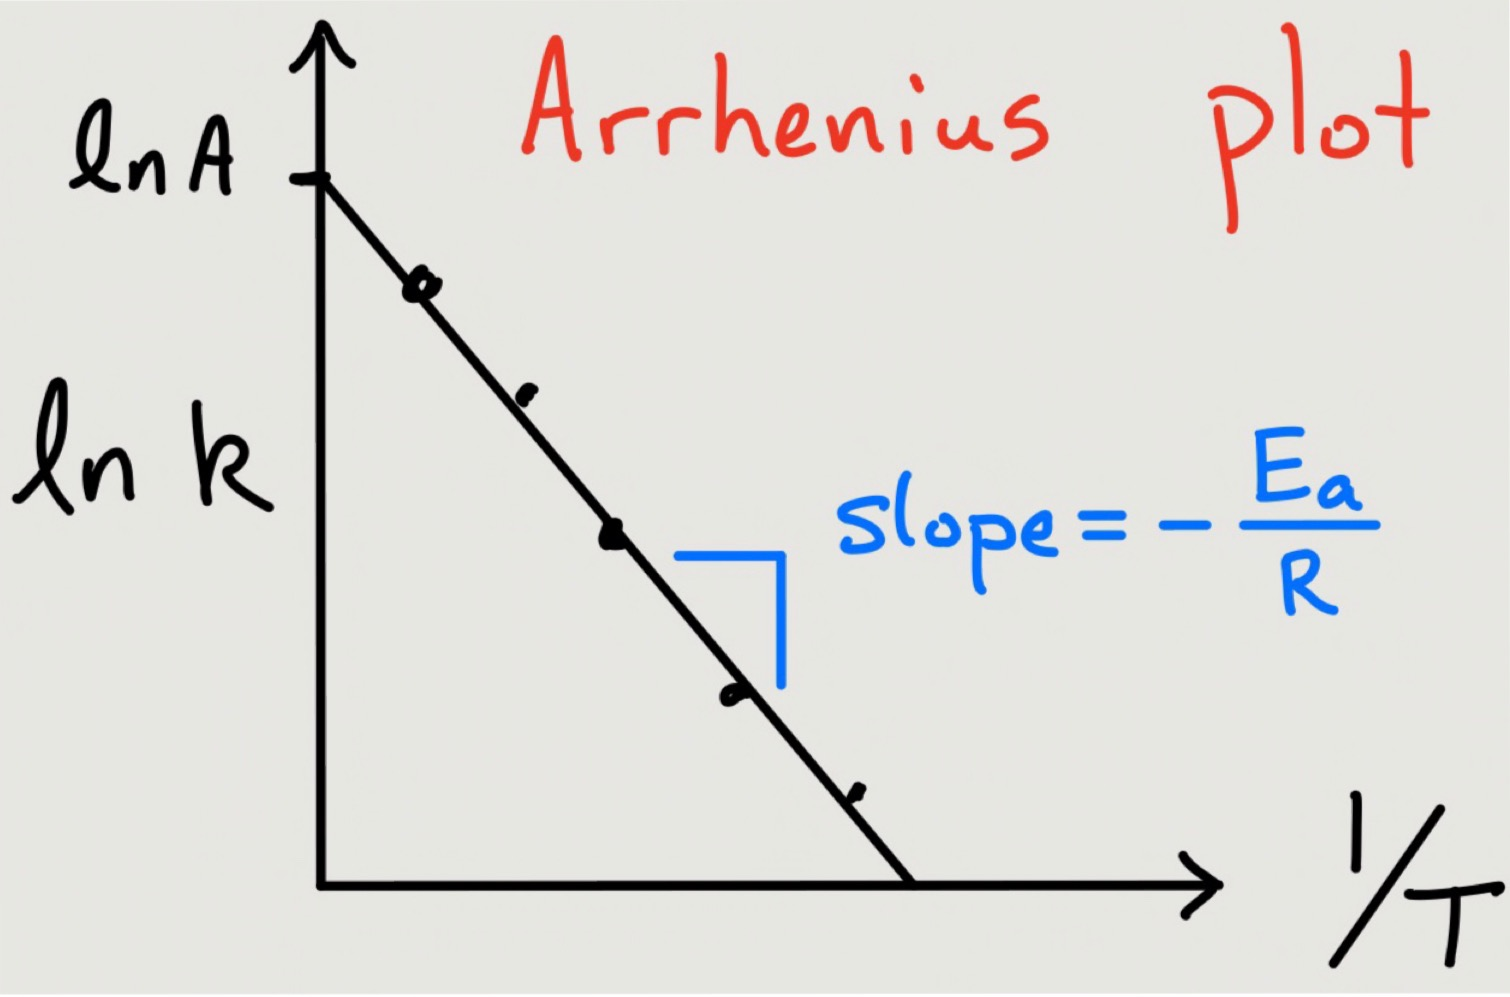
\includegraphics[width = 0.95\linewidth]{images/Arrhenius_Plot.jpeg}\\
    \fbox{$ln(k) ) \frac{-E_a}{R} \frac{1}{T} + ln(A)$}\\
    \textbf{Multistep Reaction}\\
    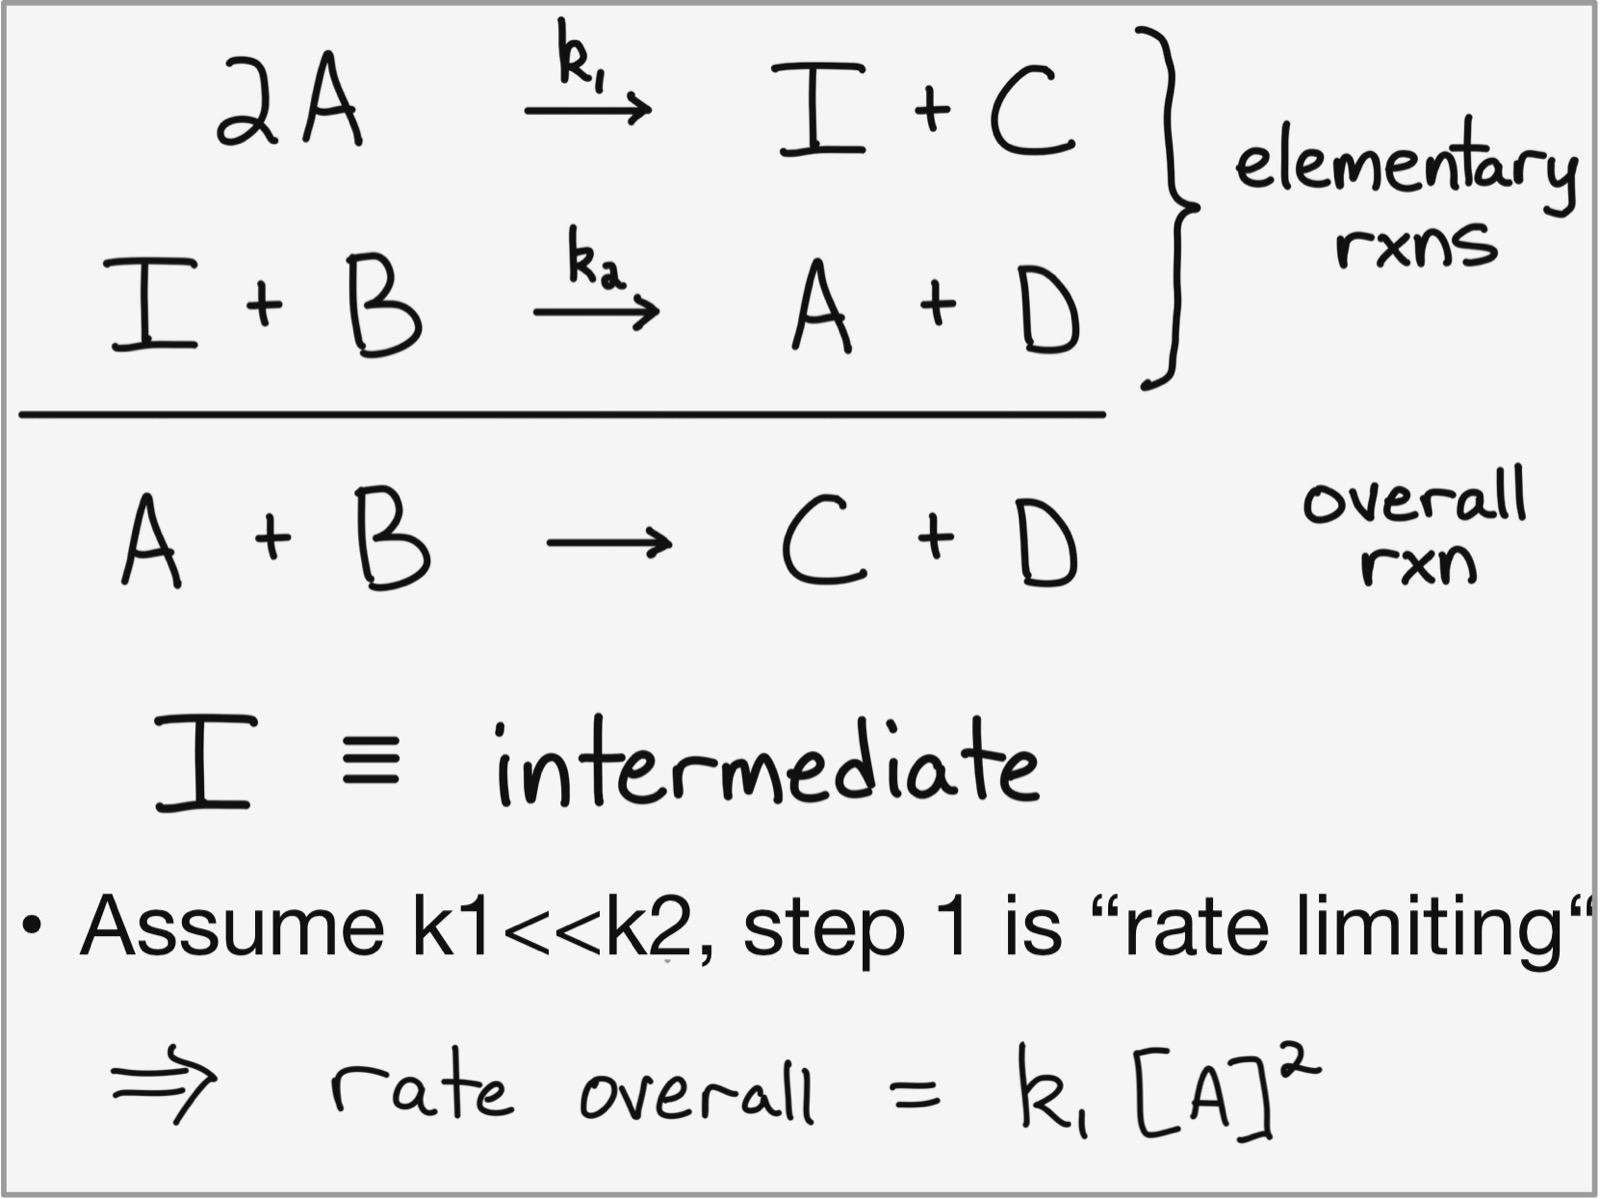
\includegraphics[width = 0.95\linewidth]{images/Multistep_Reaction.jpeg}
\end{center}
\end{minipage} 
\umbruch
%---------------------------------------
%8. Acid-Base Chemistry
%---------------------------------------
\section{Acid-Base Chemistry}
%---------------------------------------
%8.1 Chemical Equilibrium
%---------------------------------------
\subsection{Chemical Equilibrium}
\begin{minipage}{0.55\linewidth}
\textbf{Law of Mass Action}\\
\fbox{\begin{varwidth}{\textwidth}
$\alpha A + \beta B \rightleftharpoons \gamma C + \delta D$ \hspace{30pt} $K_p = K_c (RT) ^{\Delta n}$\\
\textbf{Molarity Concentrations} \hspace{15pt} \textbf{Partial Pressures}\\
$K_c = \frac{[C]^{\gamma} [D] ^{\delta}}{[A]^{\alpha} [B] ^{\beta}}$ \hspace{36pt} $K_p = \frac{(P_c)^{\gamma} (P_D)^{\delta}}{(P_A)^{\alpha} (P_B)^{\beta}}$\\
$K >> 1$ Equil. on RHS \hspace{24pt} $K << 1$ Equil. on LHS
\end{varwidth}}    
\end{minipage}
\begin{minipage}{0.3\linewidth}
    $\circ$ $\Delta n \equiv$ change in moles between products and reactants\\
    $\circ R = 0.08314 \frac{L\cdot bar}{mol \cdot K}$
\end{minipage}
\begin{minipage}{0.3\linewidth}
    \textbf{Reaction Quotient}\\
    \fbox{$Q = \frac{[C]^{\gamma} [D] ^{\delta}}{[A]^{\alpha} [B] ^{\beta}}$}
\end{minipage}
\begin{minipage}{0.6\linewidth}
    $\circ$ If $Q < K$: forward rxn forms more products\\
    $\circ$ If $Q > K$: reverse rxn forms more reactants\\
    $\circ$ For system to come to equilibrium $Q = K$
\end{minipage}
\vspace{1pt}\\
\textbf{Types of Equilibria}\\
$\circ$ Homogeneous equilibria: all substances in same phase\\
$\circ$ Heterogeneous equilbria: substances in different phases (exclude pure solids and pure liquids from K)\\
$\circ$ For low-solubility ionic solids $K \longrightarrow K_{sp} \equiv$ solubility product
\vspace{1pt}\\
\textbf{Equilibrium Math}\\
$\circ$ reverse rxn: $K = K_{original}^{-1}$\\
$\circ$ Rxn multiplied with constant factor n: $K = K_{original}^n$\\
$\circ$ Multistep rxn: product of K's for individual steps
%---------------------------------------
%8.2 Le Châtelier's Principle
%---------------------------------------
\subsection{Le Châtelier's Principle}
\textbf{\textcolor{red}{Le Châtelier's Principle}}\\
\fbox{\begin{varwidth}{\textwidth}If a system at equilibrium is disturbed by a change in concentration, pressure or temperature, the system will shift its \\ equilibrium position so as to counter the effect of the disturbance.\end{varwidth}}
\textbf{1. Concentration}: If a substance is added to a system at equilibrium, the system reacts to consume some of the substance. If a substance is removed from the system, the system reacts to produce more of that substance. \\
\textbf{2. Pressure}: At constant temperature, reducing the volume of the gaseaous equilibrium micxture causes the system to shift in the direction that reduces the number of moles of gas.\\
\begin{minipage}{0.6\linewidth}
\textbf{3. Temperature}: When increasing the temperature of a system, the system reacts as if we added a reactant to an endothermic reaction or a product to an exothermic reaction. 
\end{minipage}
\begin{minipage}{0.39\linewidth}
\begin{center}
    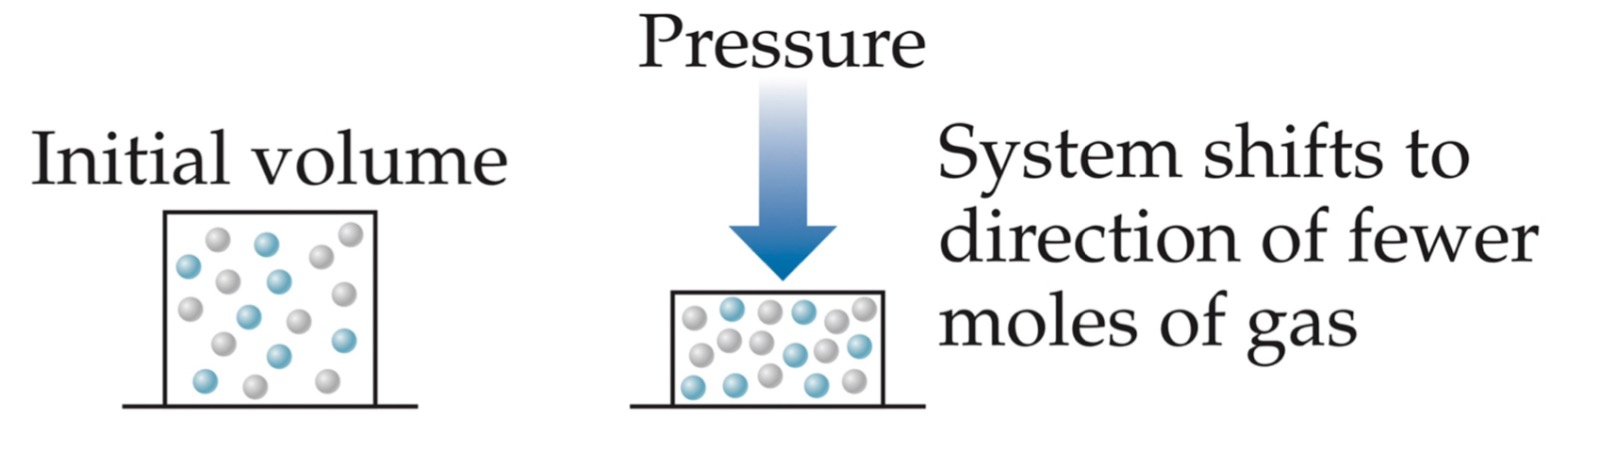
\includegraphics[width = 0.95\linewidth]{images/Pressure_le_ chatelier.jpeg}
\end{center}
\end{minipage}
\begin{center}
    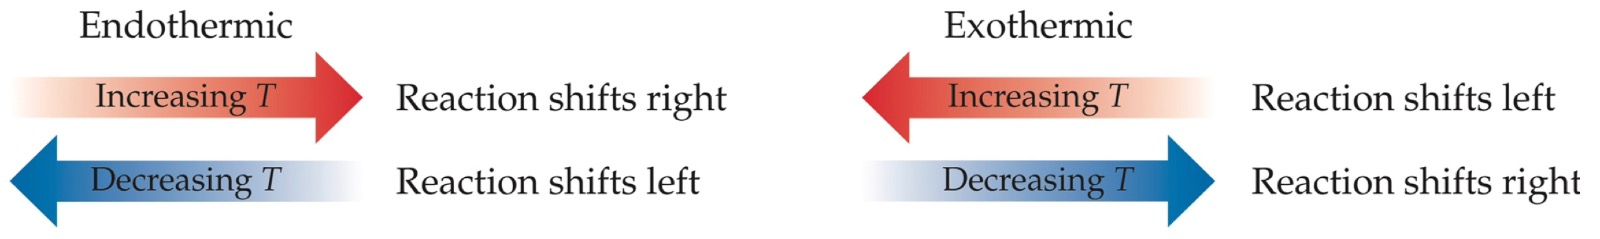
\includegraphics[width = 0.95\linewidth]{images/exothermic_vs_endothermic.jpeg}
\end{center}
$\circ$ Catalysed rxns achieve equilibrium faster, but do not change equilibrium constant K.\\
\begin{minipage}{0.69\linewidth}
\textbf{Equilibria: Connection to Thermodynamics}\\
\fbox{\begin{varwidth}{\textwidth}
$\Delta G = \Delta G^{\circ} + RTln(Q)$ \hspace{15pt} $\Delta G^{\circ} = -RTln(K)$ \hspace{15pt} $K = exp[\frac{-\Delta G^{\circ}}{RT}]$\\
At equilibrium: $\Delta G = 0, Q = K$
\end{varwidth}}
\end{minipage}
\begin{minipage}{0.3\linewidth}
$\Delta G^{\circ} at STP$\\
$\Delta G$ not at STP
\end{minipage}
%---------------------------------------
%8.3 Brönsted Acids and Bases
%---------------------------------------
\subsection{Brönsted Acids and Bases}
\begin{minipage}{0.45\linewidth}
\textbf{Acids}\\
Acids are substances that ionize in water to form \\
hydrogen cations ($H^{+}$ donors)\\
\textbf{e.g.}\\
\fbox{\begin{varwidth}{\textwidth}
$H_2SO_4(aq) \longrightarrow H^{+}(aq) + HSO_4^{-}(aq)$\\
$HSO_4^{-}(aq) \rightleftharpoons H^{+}(aq) + SO_4^{2-} (aq)$
\end{varwidth}}
\end{minipage}
\begin{minipage}{0.45\linewidth}
\textbf{Bases}\\
Bases are substances that accept 
hydrogen cations \\
($H^{+}$ acceptors). Bases produce $OH^{-}$ when dissolved in water.\\
\textbf{e.g}\\
\fbox{\begin{varwidth}{\textwidth}
$H_2O (l) + NH_3 (aq) \rightleftharpoons OH^{-} (aq) + NH_4^{+} (aq)$
\end{varwidth}}
\end{minipage}\\
\begin{minipage}{0.6\linewidth}
\textbf{Autoionization of water (ion-product constant)}\\
\fbox{$K_w = [H_3O^{+}][OH^{-} = [H^{+}][OH^{-}] = 1.0 \cdot 10^{-14}$ (at $25 ^{\circ}C$)}\\    
\end{minipage}
\begin{minipage}{0.30\linewidth}
    \textbf{Common-Ion Effect:} Add common ion to manipulate acid-base equilibrium\\
    \textbf{Buffers}: Protect against pH disturbances (comprised of acid and base)
\end{minipage}\\
\textbf{Equilibrium constants}\\
\begin{minipage}{0.5\linewidth}
    \fbox{\begin{varwidth}{\textwidth}
    $K_C \equiv K_a = \frac{[A^{-}][H_3O^{+}]}{[HA]} \equiv$ acid-dissociation constant\\
    $[HA]$: acid \hspace{5pt} $[A^{-}]$: conjugate base
\end{varwidth}}
\end{minipage}
\begin{minipage}{0.49\linewidth}
 \fbox{\begin{varwidth}{\textwidth}
    $K_C \equiv K_a = \frac{[HB^{+}][OH^{-}]}{[B]} \equiv$ base-dissociation constant\\
    $[HB^{+}]$: conjugate acid \hspace{5pt} $[B]$: base
\end{varwidth}}   
\end{minipage}\\
\fbox{\begin{varwidth}{\textwidth}
$\circ$ \textbf{Weak acid}: $K_a << 1$, equilibrium at $HA$\\
$\circ$ \textbf{Strong acid}: $K_a >> 1$, equilibrium at $A^{-}$ (completely ionized, arrow only in forward direction)
\end{varwidth}}
%---------------------------------------
%8.4 pH-, pOH-, pKa-, pKb- scales 
%---------------------------------------
\subsection{pH-, pOH-, pKa-, pKb- Scales}
\fbox{\begin{varwidth}{\textwidth}
$pH = -log[H^{+}] = - log[H_3O^{+}] = -log[\frac{K_w}{[OH^{-}]}$
\end{varwidth}}
\hspace{10pt}
\fbox{\begin{varwidth}{\textwidth}
$pOH = -log[OH^{-}] =  = -log[\frac{K_w}{[H_3O^{+}]}$
\end{varwidth}}\\
\fbox{\begin{varwidth}{\textwidth}
$-log([H^{+}]) + (-log([OH^{-}])) = -log (K_w)$ 
\end{varwidth}}
\hspace{15pt}
\fbox{\begin{varwidth}{\textwidth}
$pH + pOH = 14.00$ (at $25 ^{\circ}C$)
\end{varwidth}}\\
\fbox{\begin{varwidth}{\textwidth}
$pK_a = -log(K_a)$
\end{varwidth}}
\hspace{10pt}
\fbox{\begin{varwidth}{\textwidth}
$pK_b = -log(K_b)$
\end{varwidth}}
\hspace{10pt}
\fbox{\begin{varwidth}{\textwidth}
$pK_a + pK_b = pK_w = 14.00$ (at $25 ^{\circ}C$)
\end{varwidth}}
\begin{center}
    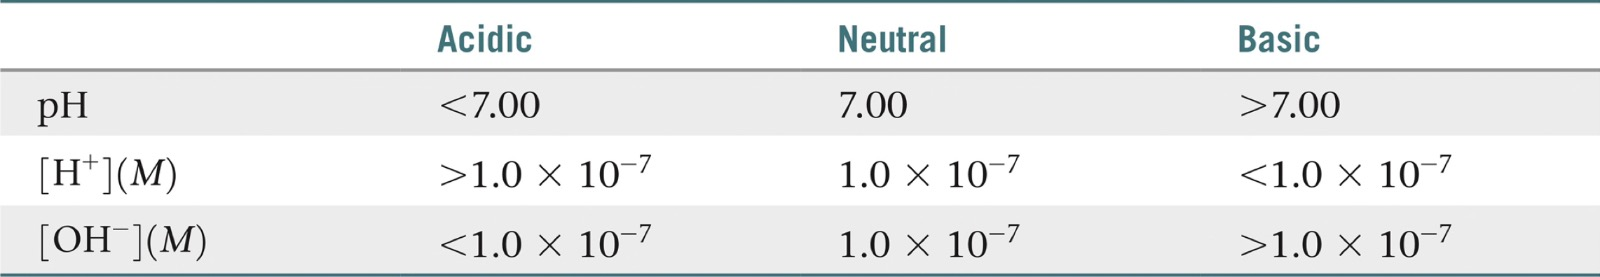
\includegraphics[width = 0.90\linewidth]{images/pH, pOH.jpeg}
\end{center}
%---------------------------------------
%9 Redox Reactions/ Electrochemistry 
%---------------------------------------
\section{Redox Reactions/ Electrochemistry }
%---------------------------------------
%9.1 General
%---------------------------------------
\subsection{General}
$\circ$ Reaction where transfers of electrons occur\\
$\circ$ \textbf{Oxidation}: Lose an electron, oxidation number is increased (reducing agent is oxidized)\\
$\circ$ \textbf{Reduction}: Gain an electron, oxidation number is reduced (oxidizing agent is reduced)\\
\begin{center}
    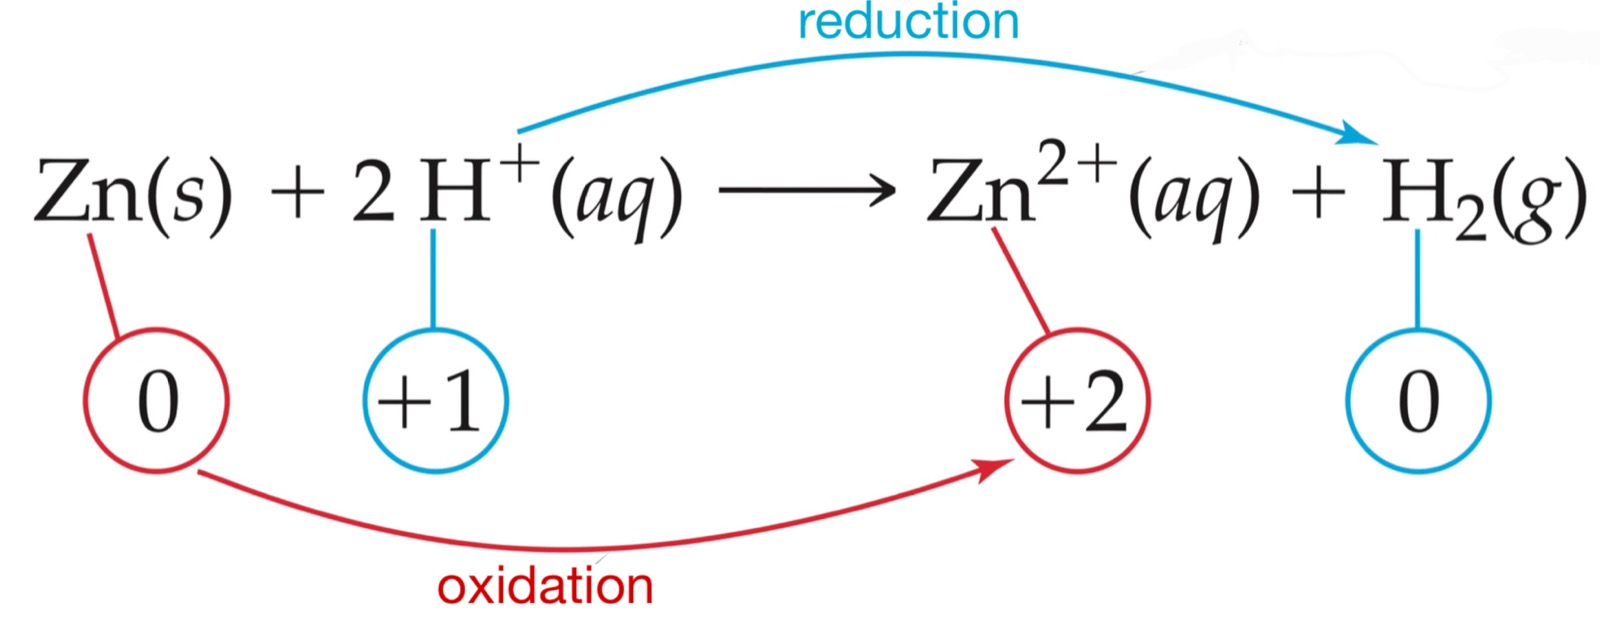
\includegraphics[width = 0.7\linewidth]{images/Redox_Reaction.jpeg}
\end{center}
%---------------------------------------
%9.2 Balancing Redox Reactions
%---------------------------------------
\umbruch
\subsection{Balancing Redox Reactions}
\textbf{How to balance redox reactions in acidic aqueous solutions}\\
\fbox{\begin{varwidth}{\textwidth}
1. Divide reactions into oxidation half-reaction and reduction half-reaction
\vspace{1pt}\\
2. Balance each half-reaction
\vfill \hspace{10pt}- First, balance elements other than $H$ and $O$
\vfill \hspace{10pt}- Next, balance $O$ atoms by adding $H_2O$ as needed
\vfill \hspace{10pt}-Then, balance $H$ atoms by adding $H^{+}$ as needed
\vfill \hspace{10pt}-Finally, balance charge by adding e's as needed \\
3. Multiply two half-reactions by integers to equate the electrons lost and gained\\
4. Add half-reactions and, if possible, cancel specieas appearing on both sides\\
5. Check to make sure atoms and charges are balanced. 

\end{varwidth}}
\vspace{3pt}

\textbf{How to balance redox reactions in basic aqueous solutions}\\
\fbox{\begin{varwidth}{\textwidth}
1. Balance half-reactions as if they occured in acidic solution (steps 1 and 2)\\
2. Count number of $H^{+}$ in each half-reaction, and add same number of $OH^{-}$ to each side
\vfill \hspace{10pt}- Why? Neutralizing $H^{+}$ with $OH^{-}$ 
\vfill \hspace{10pt}- Equal $H^{+}$ and $OH^{-}$ on same side form $H_2O$
\vfill \hspace{10pt}- Cancel any $H_2O$ appearing on both sides\\
3. Multiply two half-reactions by integers to equate the electrons lost and gained\\
4. Add half-reactions and, if possible, cancel specieas appearing on both sides\\
5. Check to make sure atoms and charges are balanced. 
\end{varwidth}}
%---------------------------------------
%9.3 Voltaic Cell/Battery
%---------------------------------------
\subsection{Voltaic Cell/ Battery}
\textbf{Voltaic Cell/ Battery}\\
\fbox{\begin{varwidth}{\textwidth}
$\circ$ \textbf{Activity series}: any metal is oxidized by metals below it (spontaneous).\\
$\circ$ \textbf{Components}:\\
1. \textbf{Electrodes}: solid metals connected to external circuit. Anode loses mass, whilst cathode gains mass (deposition). \\
2. \textbf{Electrolyte}: liquid with ions that can conduct electrical current\\
3. \textbf{Salt bridge}: tube containing electrolyte solution facilitating ion migration 
\end{varwidth}}
\begin{center}
    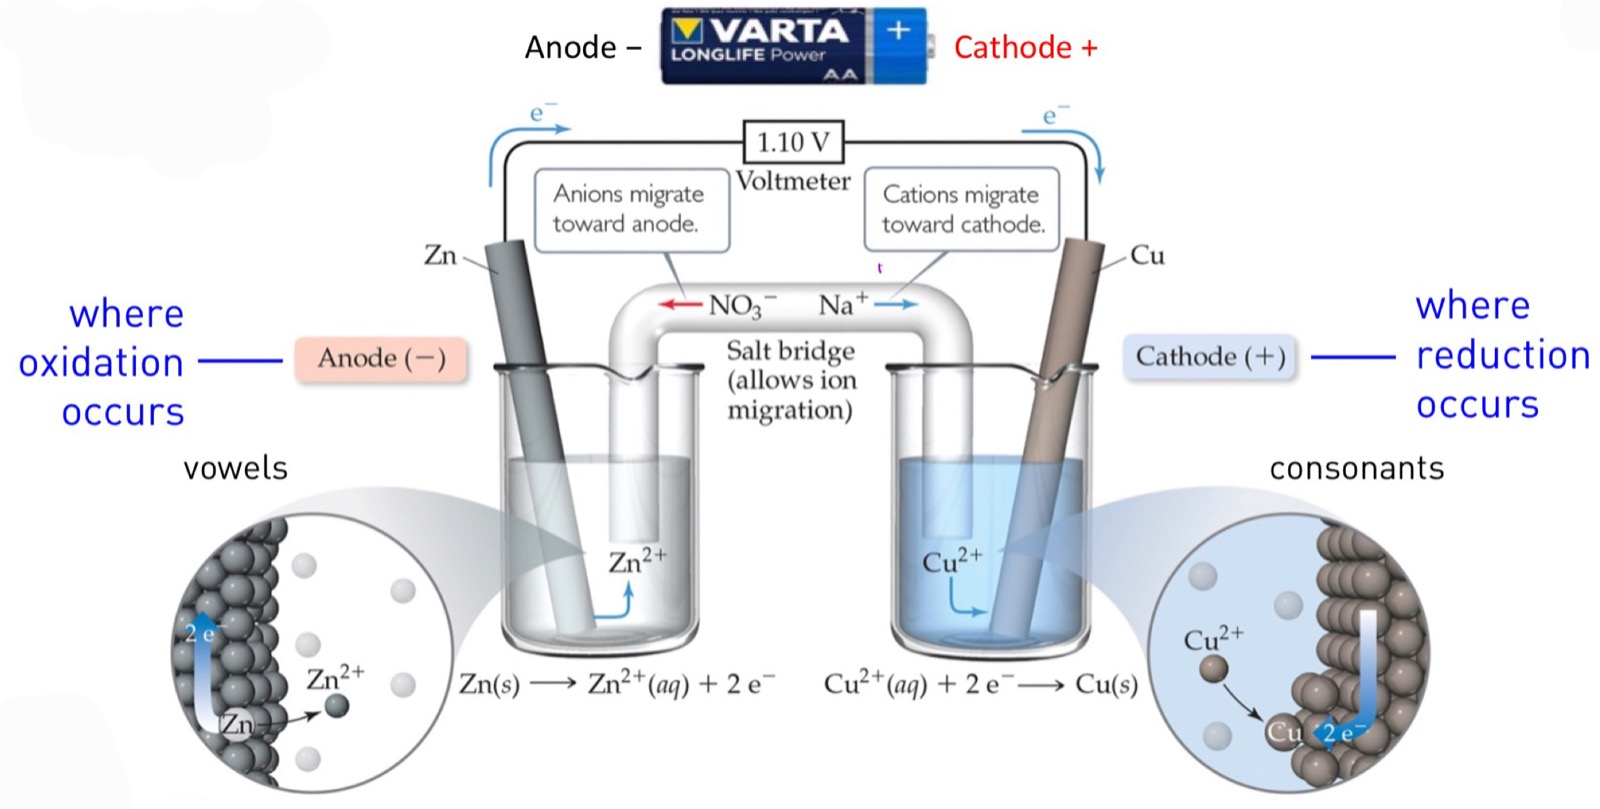
\includegraphics[width = 0.9\linewidth]{images/Voltaic_Cell.jpeg}
\end{center}
\begin{minipage}{0.3\linewidth}
    \textbf{Cell Potentials}\\
    \fbox{$ 1V = \frac{1.6\cdot 10^{-19} J}{1.6 \cdot 10^{-19} C}$}
\end{minipage}
\begin{minipage}{0.6\linewidth}
    \textbf{Cell Voltage at STP (Thermodynamics)}\\
    \fbox{$E_{cell}^{\circ} = E_{red}^{\circ}$ (cathode) $ E_{red}^{\circ}$ (anode)}
\end{minipage}\\

\begin{minipage}{0.6\linewidth}
\textbf{Gibbs Free Energy}\\
\fbox{\begin{varwidth}{\textwidth}
$\Delta G^{\circ} = -nFE^{\circ}$ \hspace{15pt} $E^{\circ} = \frac{\Delta G^{\circ}}{-nF} = \frac{-RTln(K)}{-nF} = \frac{RT}{nF}ln(K)$
\end{varwidth}}\\
If $E_{cell}^{\circ} > 0, \Delta G^{\circ} < 0 \longrightarrow$ rxn is spontaneous
\end{minipage}
\begin{minipage}{0.39\linewidth}
    $\Delta G^{\circ} \equiv J/mol$ of rxn\\
    $F = 96485 \frac{C}{mol} \equiv$ Faraday's constant\\
    $n \equiv$ moles of e's transferred in rxn\\
    $K \equiv$ Equilibrium constant
\end{minipage}
%---------------------------------------
%10. Appendix
%---------------------------------------
\section{Appendix}
$\circ$ \textbf{Intensive Properties}: Do no depend on the system size or the amount of material. (e.g. temperature, refractive index, density, $E_{cell}^{\circ}$\\
$\circ$ \textbf{Extensive Properties}: Depend on system size. (e.g. mass, volume, entropy)
\vspace{3pt}\\
\textbf{Atoms}\\
$\circ$ \textbf{Atomic Number}: \# of protons in atom of particular element\\
$\circ$ \textbf{Isotopes}: Same element with different \# neutrons\\
$\circ$ \textbf{Mass Number}: \# of protons and neutrons\\
$\circ$ \textbf{Atomic Mass Scale}: $\prescript{12}{6}{C} \equiv 12u$ \hspace{7pt} $m_p = 1.0073 u$ \hspace{7pt} $m_n = 1.0087 u$ \hspace{7pt} $m_e = 5.486\cdot 10^{-4} u$ \hspace{7pt} $1u = 1.6605 \cdot 10^{-27} kg$\\
$\circ$ \textbf{Atomic Weight}: Average atomic mass of all isotopes of an element, weighted by their natural abundance in atomic mass units\\
$\circ$ \textbf{Atomic Mass}: The mass of an atom's electrons, protons and neutron in atomic mass units
\vspace{3pt}\\
\textbf{Metathesis and Precipitation Reactions}:
$\circ$ \textbf{Metathesis}: Two ionic solids dissolve and exchange partners\\
$\circ$ If cation/ anion pair is strongly attracted, a solid preciptate is formed. 


\section{Author's notes}
I neither guarantee that the following summary is complete nor absolutely correct. Please forward any corrections or suggestions for improvements to joetan@ethz.ch. This summary was written specifically for Prof. David Norris' Chemistry course.
Should you wish to publish an improved version with your own notes and changes, please make clear that it is not the original version. 
\\
Viel Erfolg! Glück brucht mer nur wemers nöd chan. 

\end{document}
